\documentclass[10pt,letterpaper]{article}
\usepackage[top=0.85in,left=2.75in,footskip=0.75in]{geometry}

% amsmath and amssymb packages, useful for mathematical formulas and symbols
\usepackage{amsmath,amssymb}

% Use adjustwidth environment to exceed column width (see example table in text)
\usepackage{changepage}

% Use Unicode characters when possible
\usepackage[utf8x]{inputenc}

% textcomp package and marvosym package for additional characters
\usepackage{textcomp,marvosym}

% cite package, to clean up citations in the main text. Do not remove.
\usepackage{cite}

% Use nameref to cite supporting information files (see Supporting Information section for more info)
\usepackage{nameref,hyperref}

% line numbers
\usepackage[right]{lineno}

% ligatures disabled
\usepackage{microtype}

% color can be used to apply background shading to table cells only
\usepackage[table]{xcolor}

% array package and thick rules for tables
\usepackage{array}

\usepackage{subfig}
% \usepackage[demo]{graphicx}


% Remove comment for double spacing
\usepackage{setspace} 
%\doublespacing

\usepackage{csquotes}
\usepackage{dirtytalk}
\usepackage[english]{babel}
\usepackage{hyperref}
\hypersetup{
    colorlinks=true,
    citecolor=blue,
    linkcolor=blue,
    urlcolor=blue,
    pdftitle={Algorithmic Bias Media Model},
    pdfpagemode=FullScreen}
\urlstyle{same}


% Bold the 'Figure #' in the caption and separate it from the title/caption with a period
% Captions will be left justified
\usepackage[aboveskip=1pt,labelfont=bf,labelsep=period,justification=raggedright,singlelinecheck=off]{caption}

% Use the PLoS provided BiBTeX style
\bibliographystyle{plos2015}



% Header and Footer with logo
\usepackage{lastpage,fancyhdr,graphicx}
\usepackage{subfig}

\usepackage{epstopdf}
%\pagestyle{myheadings}
\pagestyle{fancy}
\fancyhf{}
%\setlength{\headheight}{27.023pt}
%\lhead{\includegraphics[width=2.0in]{PLOS-submission.eps}}
\rfoot{\thepage/\pageref{LastPage}}
\renewcommand{\headrulewidth}{0pt}
\renewcommand{\footrule}{\hrule height 2pt \vspace{2mm}}
\fancyheadoffset[L]{2.25in}
\fancyfootoffset[L]{2.25in}
\lfoot{\today}

%% Include all macros below

\newcommand{\lorem}{{\bf LOREM}}
\newcommand{\ipsum}{{\bf IPSUM}}

\begin{document}
%
\title{Mean-field analysis of the effects of mass media presence on Deffuant-Weisbuch model with Algorithmic Bias.}
%
%\titlerunning{Abbreviated paper title}
% If the paper title is too long for the running head, you can set
% an abbreviated paper title here
%
% Author Orchid ID: enter ID or remove command

% \author{Frank Dignum $^{1}$\orcidA{}, Dino Pedreschi $^{2}$\orcidB{}, Giuliano Cornacchia $^{2,4}$\orcidC{}, \\
%                 Virginia Morini$^{2,4}$\orcidD{}, Valentina Pansanella$^{3,4}$\orcidE{}}

%\author{Frank Dignum\inst{1}\orcidA{} \and
%Dino Pedreschi\inst{2,3}\orcidID{0000-0003-4801-3225} \and  
%Giuliano Cornacchia\inst{3}\orcidID{0000-0003-2263-7654} \and
%Virginia Morini\inst{4}\orcidID{0000-0002-7692-8134} \and
%Valentina Pansanella\inst{5}\orcidID{0000-0001-8106-7677}}
%
% \authorrunning{F. Dignum et al.}
% First names are abbreviated in the running head.
% If there are more than two authors, 'et al.' is used.
% %
% \institute{Umeå University, Sweden \\ \email{dignum@cs.umu.se} \\  \and University of Pisa, Italy  \\ \email{dino.pedreschi@unipi.it} \\
% \email{\{giuliano.cornacchia,virginia.morini\}@phd.unipi.it} \\ \and 
% Scuola Normale Superiore, Pisa, Italy \\
% \email{valentina.pansanella@sns.it}\\ \and
%  KDD Lab ISTI-CNR, Pisa, Italy}
%\url{http://www.springer.com/gp/computer-science/lncs} }
%ABC Institute, Rupert-Karls-University Heidelberg, Heidelberg, Germany\\
%\email{\{abc,lncs\}@uni-heidelberg.de}}
%
\maketitle              % typeset the header of the contribution
%
\begin{abstract}
People often form their opinion by accessing and discussing contents shared on social networking websites, which is a mixture of their friends shared opinions and content distributed by main stream media sources like online newspapers.
While OSN have fostered information access and diffusion, they represent optimal environments for the proliferation of polluted contents, which is argued to be one of the co-causes of polarization/radicalization. 
Moreover, recommendation algorithms - intended to enhance platform usage - are likely to augment such phenomena, generating the so called \emph{Algorithmic Bias}. In this work, we study the effects of the combination of social influence and mass media influence on the dynamics of opinion evolution in a biased online environment, using a recent bounded confidence opinion dynamics model with algorithmic bias as baseline and adding the possibility to interact with one or more media outlets, modelled as stubborn agents.
\end{abstract}
%
%
%

\section{Introduction}
Opinions and beliefs shape individual behaviour, which drives human actions, and a society's collective behaviour, influencing politics, public health, and the environment. Changes in public opinion - even the formation of committed minorities - may profoundly affect decision-makers and politics: a recent example is the temporary suspension of the Oxford-AstraZeneca vaccine during March 2021, which has costed a slowdown in the vaccination strategy. Opinion evolution is a complex process, depending on social interactions with peers and on the information people collect from external sources. 
The way in which one processes such information, however, is far from being perfectly rational and is highly influenced by psychological factors and cognitive biases. 
Online social media and networks are increasingly used as an alternative source of news and information, alongside traditional media (which are still the main source up to this day), but also as an environment to express personal opinions, engage in discussion, share content from other sources with one's personal network. These environments are ruled by algorithms that filter and personalise each user's experience accordingly to their and their friends' past behaviour, which were intended to maximise users engagement and enhance platform usage. However, it is theorised that filtering algorithms and recommender systems are likely to create an algorithmic bias, i.e. showing people only narratives that are aligned with their own existing beliefs, stimulating a positive feedback loop further reducing the amount of diversity in the user experience - possibly contributing to the creation and maintenance of echo chambers and filter bubbles. Although personalization is essential in information-rich environments to allow people to find what they are looking for and increase user engagement, there is great concern about the negative consequences of algorithmic filtering such as polarisation and radicalisation. 
Therefore, understanding opinion dynamics and how these different factors play a role in the final state of a population is essential to understand human behaviour, but also to define mitigation strategies to avoid unintended consequences, which may have negative effects on the well-being of the societies and also be a threat to democracy itself. 
While, as previously stated, social influence plays a significant role in shaping our culture, ideology and opinion spectrum; reading news or being the target of mass political propaganda may affect us, and models of opinion dynamics should consider it when addressing the study of opinion formation. Also, external agents (i.e., a government, a company, a group of terrorists) may be interested in shifting the public's opinion concerning a specific topic. Propaganda or other actions can be exploited to promote one stance over the others \cite{Franke2015StrategiesOP}, or to achieve a particular value for the consensus opinion \cite{Lorenz2007AboutTP}, or maybe to prevent people from reaching more extreme opinions \cite{Timothy2017HowDP} to avoid the consequent risks.
The present work aims to understand the role of mass media in an environment with a recommender system and algorithmic bias with an opinion dynamics modelling approach, assuming a mean-field context (e.g., all individuals can interact among them without any social restrictions). 
Adopting such controlled environments, used to simulate the social structure among a population of interacting individuals, we analyse the behaviours of the Algorithmic Bias model\cite{Srbu2019AlgorithmicBA} (e.g., an extension of the Deffuant-Weisbuch\cite{DW00} opinion dynamics model) with the presence of mass media modelled as stubborn agents.

\smallskip
The paper is organised as follows. In section \ref{sec:modeldefinition} we introduce the algorithmic bias model, and we describe the change in the interaction rules due to the presence of mass media. Section \ref{sec:results} discusses the main finding of our simulations, finally section \ref{sec:conlcusion} concludes the paper while opening to future investigations.

\section{Model definition}
\label{sec:modeldefinition}
Considering such a complex scenario, the present work aims to deepen the AB model's behaviour analysis and understand how biased interactions with mass media may influence the outcomes of the dynamical process. 

Nowadays, online social networks have become the primary source of information and an excellent platform for 
discussions and 
opinion exchanges. 
However, the flow of content that each user sees is organised by algorithms that are built to maximise platform usage: from this, it comes to the hypothesis that there is an algorithmic bias (also called algorithmic segregation) since these contents are selected based on users' precedent actions on the platform or the web, 
reinforcing the human tendency to interact with content confirming their beliefs (confirmation bias). 
It is a human tendency to prefer interaction with information/content/discussions that confirm their narrative (a phenomenon known as confirmation bias), so users tend to interact more with this kind of content rather than go and face evidence that puts in discussion their beliefs. 
Therefore, it is in the service provider's interest to deliver its contents in a targeted way.


To introduce in the study of opinion dynamics the idea of a recommender system generating an algorithmic bias, we started from a recent extension of the well-known Deffuant-Weisbuch model (DW-model henceforth), proposed in \cite{Srbu2019AlgorithmicBA} (Algorithmic Bias model or AB model, hereafter).

In the Algorithmic Bias model, we have a population of $N$ agents, where each agent $i$ has a continuous opinion $x_{i} \in [0,1]$. 
At every discrete time step the model randomly select a pairwise $(i, j)$, and, if their opinion distance is lower than a threshold $\epsilon$, $|x_{i} - x_{j}| \leq \epsilon$, then the two agents change their opinion according to the following rule:
\begin{equation}
\begin{aligned} 
    \label{eq:updateDW}
    x_{i}(t+1) &=  x_{i} + \mu(x_{j}-x_{i}) \\ 
    x_{j}(t+1) &=  x_{j} + \mu(x_{i}-x_{j}).
\end{aligned}   
\end{equation}

The parameter $epsilon \in [0,1]$ represents the confidence bound of the population, which is assumed to be constant throughout all agents.
A population with a low $epsilon$ is closed-minded. Individuals can only be influenced by those with similar opinions; a high $epsilon$, on the other hand, results in an open-minded population because two agents can influence each other even if their initial opinions are very different.
The parameter $\mu \in (0, 0.5]$ is a convergence parameter, modelling the strength of the influence the two individuals have on each other or, in other words, how much they change their opinion after the interaction. 
Even if there is no reason to assume that $\epsilon$ should be constant across the population or at least symmetrical in the binary encounters, this parameter is always considered equal for every agent. 
The numerical simulations of this model show that the qualitative dynamic is mainly dependent on $\epsilon$: as $\epsilon$ grows, the number of final opinion clusters decreases. 
As for $\mu$ and $N$, these parameters tend to influence only the time to convergence and the final opinion distribution width. 

The AB model introduces another parameter to model the algorithmic bias: $\gamma \geq 0$. This parameter represents the filtering power of a generic recommendation algorithm: if it is close to $0$, the agent has the same probability of interacting with all its peers. As $\gamma$ grows, so does the probability of interacting with agents holding similar opinions, while the likelihood of interacting with those who have distant opinions decreases.
Therefore, this extended model modifies the rule to choose the interacting pair $(i, j)$ to simulate a filtering algorithm's presence. An agent $i$ is randomly picked from the population, while $j$ is chosen from $i$'s peers according to the following rule:
\begin{eqnarray}             
    \label{eq:algbias}
    p_{i}(j)=\frac{d_{ij}^{-\gamma}}{\sum_{k \ne i}d_{ik}^{-\gamma}}
\end{eqnarray}
where $d_{ij} = |x_{i}-x_{j}|$ is the opinion distance between agents $i$ and $j$, so that for $\gamma = 0$ the model goes back to the DW-model.
To add the interactions with media outlets in the model we added another parameter, namely $p_m \in [0, 1]$, which indicates the probability that in addition to interacting with a neighbour, the agent also interacts with a media.  
When two agents interact, their opinions change if and only if the distance between their opinions is less than the parameter $\epsilon$, i.e., \(|x_{i}-x_{j}| \leq \epsilon \), according to Eq.~\ref{eq:updateDW}.

\begin{figure}
    \centering
    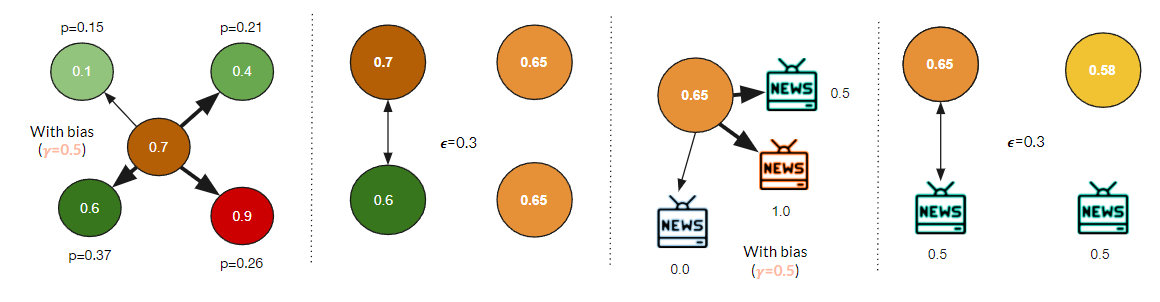
\includegraphics[width=\textwidth]{figures/example.PNG}
    \caption{\textbf{Example interaction.}}
    \label{fig:example}
\end{figure}
If one of the agents is a mass media, in the equation \ref{eq:updateDW} its opinion don't change and only the user-agent opinion shifts towards the mean. 
Our goal here is to understand the effects of biased media outlets that promote a certain, fixed opinion during the whole time period. Therefore, we modelled media as stubborn agents (or zealots) never changing their opinion and connected to everyone in the network, to simulate a news source accessible to everyone in the population. Figure \ref{fig:example} illustrates an example of a possible interaction (both peer-to-peer and agent-to-media) and its effects on the node’s opinion. 


\section{Analysis and results}
\label{sec:results}
We performed simulations of this model on a complete network of $100$ nodes where the initial opinions are initially uniformly distributed across the population and averaged the results over $100$ runs. Like in \cite{Srbu2019AlgorithmicBA}, to avoid undefined operations in equation \ref{eq:algbias}, when $d_{ik} = 0$ we use a lower bound $d_{\epsilon} = 10^{-4}$. 
The simulations are designed to stop when the population reaches an equilibrium, i.e., the cluster configuration will not change anymore, even if the agents keep exchanging opinions. 
We also set an overall maximum number of iterations at $10^6$. 
To better understand the differences in the final state concerning the different topologies considered, we study the model on all networks for various combinations of the parameters. 
We are interested in whether, parameters being equal, the different number and positioning of mass media and the growing interaction probability influences the final configuration, enhancing or reducing fragmentation and radicalising individuals towards more extreme opinions. 

We replicated the work of \cite{Srbu2019AlgorithmicBA} by setting a null probability to interact with the media, to define a reliable baseline for comparison. 

In the simulations, we tested the model on every possible combination of the parameters over the following values:
\begin{itemize}
    \item $p_{m}$ takes values in $\{0.0, 0.1, 0.2, 0.3, 0.4, 0.5\}$, where for $p_{m}=0$ the model becomes the AB model.
    \item $\epsilon$ takes value in $\{0.1, 0.2, 0.3, 0.4, 0.5, 1.0\}$.
    \item $\gamma$ takes value in $\{0.0, 0.5, 0.75, 1.0, 1.25, 1.5\}$ where for $\gamma = 0$ the model becomes the DW-model.
    \item $\mu = 0.5$, so whenever two agents interact, if their opinions are close enough, they update to the average opinion of the pair.
\end{itemize}

We analysed two scenarios to understand the effects of (i) one extreme media with an opinion $m_{1}=0.0$ and (ii) three media with opinions $m_{1}=0.05, m_{2}=0.5, m_{3}=0.95$. 

The AB model with mass media implementation used to carry out our experiments is the one provided by the NDlib \cite{rossetti2018ndlib} Python library\footnote{NDlib: \url{http://ndlib.rtfd.io}}.


\subsection{Experimental results}
\subsubsection{Media and bounded confidence}
To understand the results of the presence of mass media in a non-biased environment, we analysed the number of opinion clusters and the value of entropy as a function of both $p_{m}$ and $\epsilon$, setting $\gamma=0.0$. 
The behaviour of the original Deffuant-Weisbuch model is defined by the parameter $\epsilon$; when this is large enough, an initially uniformly random population converge to consensus. In contrast, as $\epsilon$ decreases, clusters emerge in the population, and their number can be approximated by $\lfloor{\frac{1}{2\epsilon}\rfloor}$, ignoring minor clusters that appear in some situations. 
%devo dire come ho fatto il clustering?
To compute the effective number of clusters, accounting for the presence of major and minor ones, we use the cluster participation ratio, as in \cite{Srbu2019AlgorithmicBA}:
\begin{eqnarray}
    \label{eq:ncluster}
    C = \frac{(\sum_{i}{c_{i}})^{2}}{\sum_{i}{c_{i}^{2}}}
\end{eqnarray}
where $c_{i}$ is the dimension of the $i$th cluster, i.e., the fraction of population we can find in that cluster. In general, for n clusters, the maximum value of the participation ratio is n and is achieved when all clusters have the same size. At the same time, the minimum can be close to 1 if one cluster contains most of the population and a tiny fraction is distributed among the other $n − 1$.
To account for situations where proper clusters may not emerge in the population - hence the effective number of clusters may fail to capture the features of the distribution - we computed the entropy of the final opinion distribution, using Shannon entropy on the discrete probability distribution, dividing the opinion spectrum into $k$ intervals of equal width and computing the probability of a node to be in the interval $i$, $p(i)$. Shannon's entropy is:
\begin{eqnarray}
    \label{eq:entropy}
    S = {-\sum{p(i)\ln p(i)}}
\end{eqnarray}

\begin{figure}
    \centering
    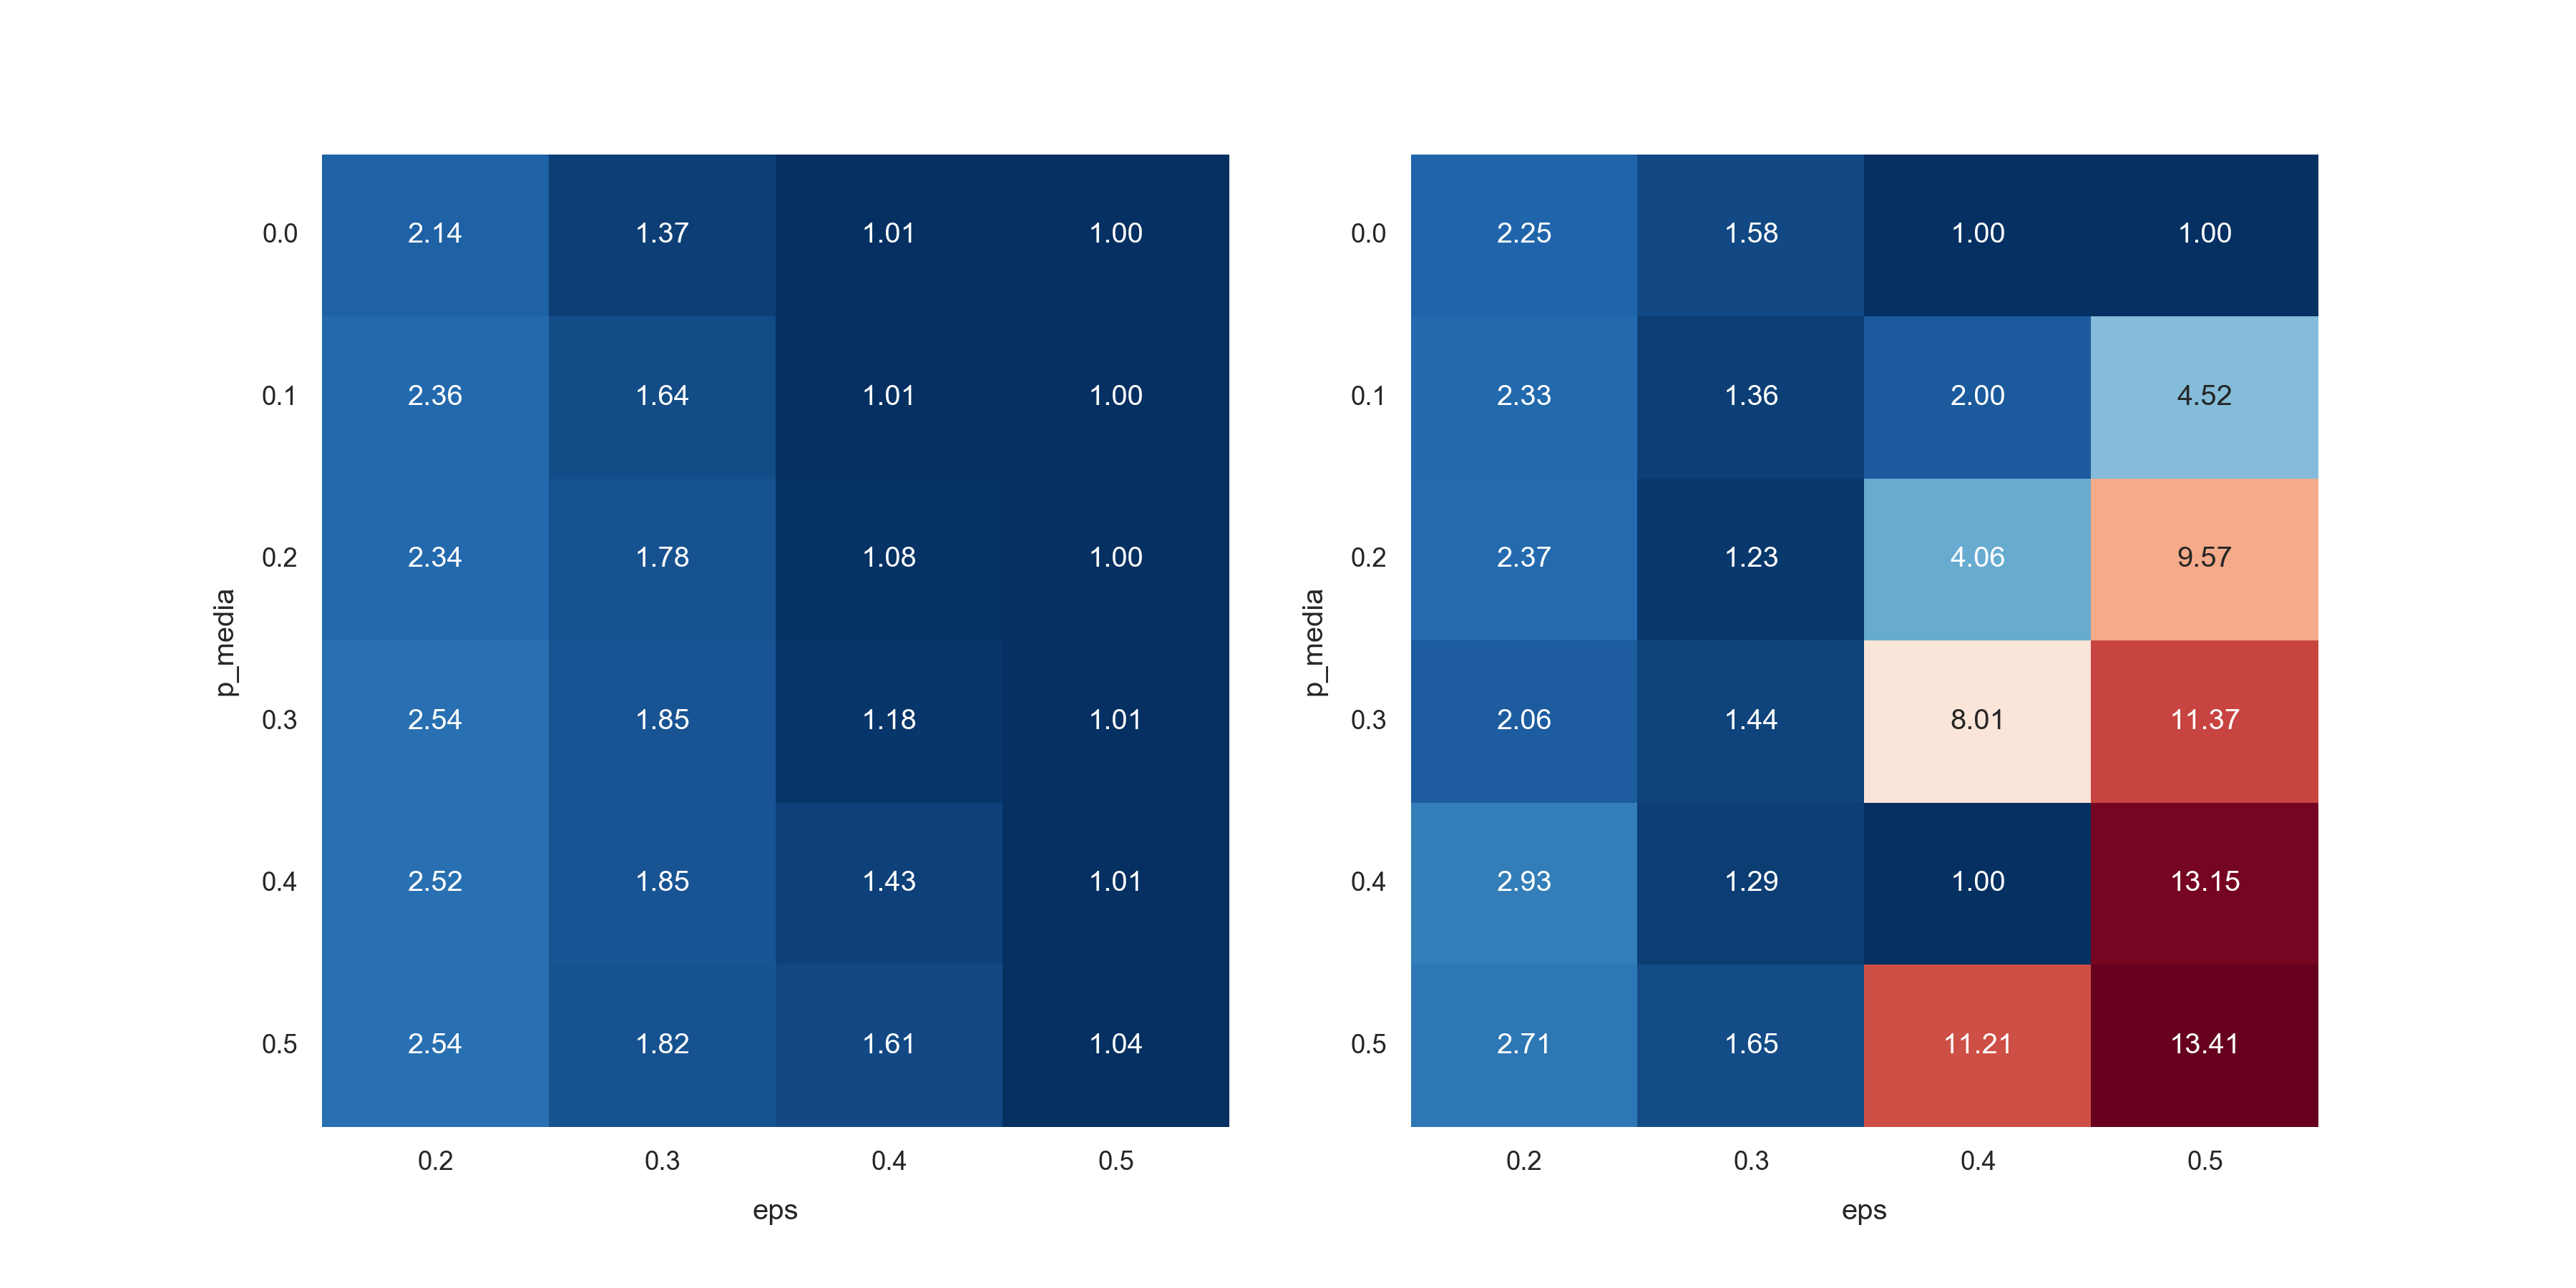
\includegraphics[width=0.8\textwidth]{figures/hm media nobias mo0.05;0.5;0.95 new_avg_ncluster groupedby_media_op.png}
    \caption{\textbf{Average number of clusters as a function of $\epsilon$ and $p_m$ in a non-biased environment.} In the figure the average number of clusters as a function of $\epsilon$ and $p_m$ is showed for both settings: with one media with opinion $m_1 = 0.0$ (left) and with three media with opinions $m_1=0.05, m_2 = 0.5, m_3=0.95$ (right). The average number of clusters grows with the increase in the probability to interact with the one extreme media, but the growth of $\epsilon$ counters this effect (left). When the medias are $3$ the increase in the level of bounded confidence has the opposite effect and exacerbates fragmentation when combined with agent-to-media interactions.}
    \label{fig:gammazero}
\end{figure}

In figure \ref{fig:gammazero} we can see the average number of clusters obtained in our simulations. The first row of both heatmaps shows the behaviour of the original Deffuant-Weisbuch model, which is then compared to the results of an increased probability to interact with the media present in the model. These plots show how increasing $p_m$ the average number of clusters increases. However, there are two very different behaviour in the two different settings. If we have only one media, a consensus is always reached for $\epsilon \geq 0.4$, and for $\epsilon \geq 0.5$ interacting with the media does not affect the number of clusters. When we consider the three-media setting, instead, a higher $\epsilon$ results in a higher fragmentation and the average number of clusters increases, instead of decreasing, compared to lower values of $\epsilon$. This happens because while $\epsilon \leq 0.3$ most of the nodes will mainly interact with only one of the media - the one closest to their present opinion - and only a few nodes will move to the opposite side of the opinion spectrum; however, when $\epsilon \ge 0.3$ many nodes at any time step can be influenced by more than one media. This creates volatile dynamics because nodes keep moving within the opinion spectrum and hardly cluster. 

\subsubsection{Biased media interactions}
% Also, the effects of the algorithmic bias, i.e., $\gamma > 0$, are different in the two different settings.\\ \\
Biasing both peer-to-peer and agent-to-media interactions, namely setting $\gamma > 0$, has very different effects in the two settings, which we will briefly describe in the remainder of this sections, using entropy, the average number of clusters, the average pairwise distance, the average number of iterations at convergence, the mean opinion and the percentage of agents attracted by each media to give a complete description of the dynamics and its results.

\textbf{One extreme media}
\begin{figure}
    \centering
    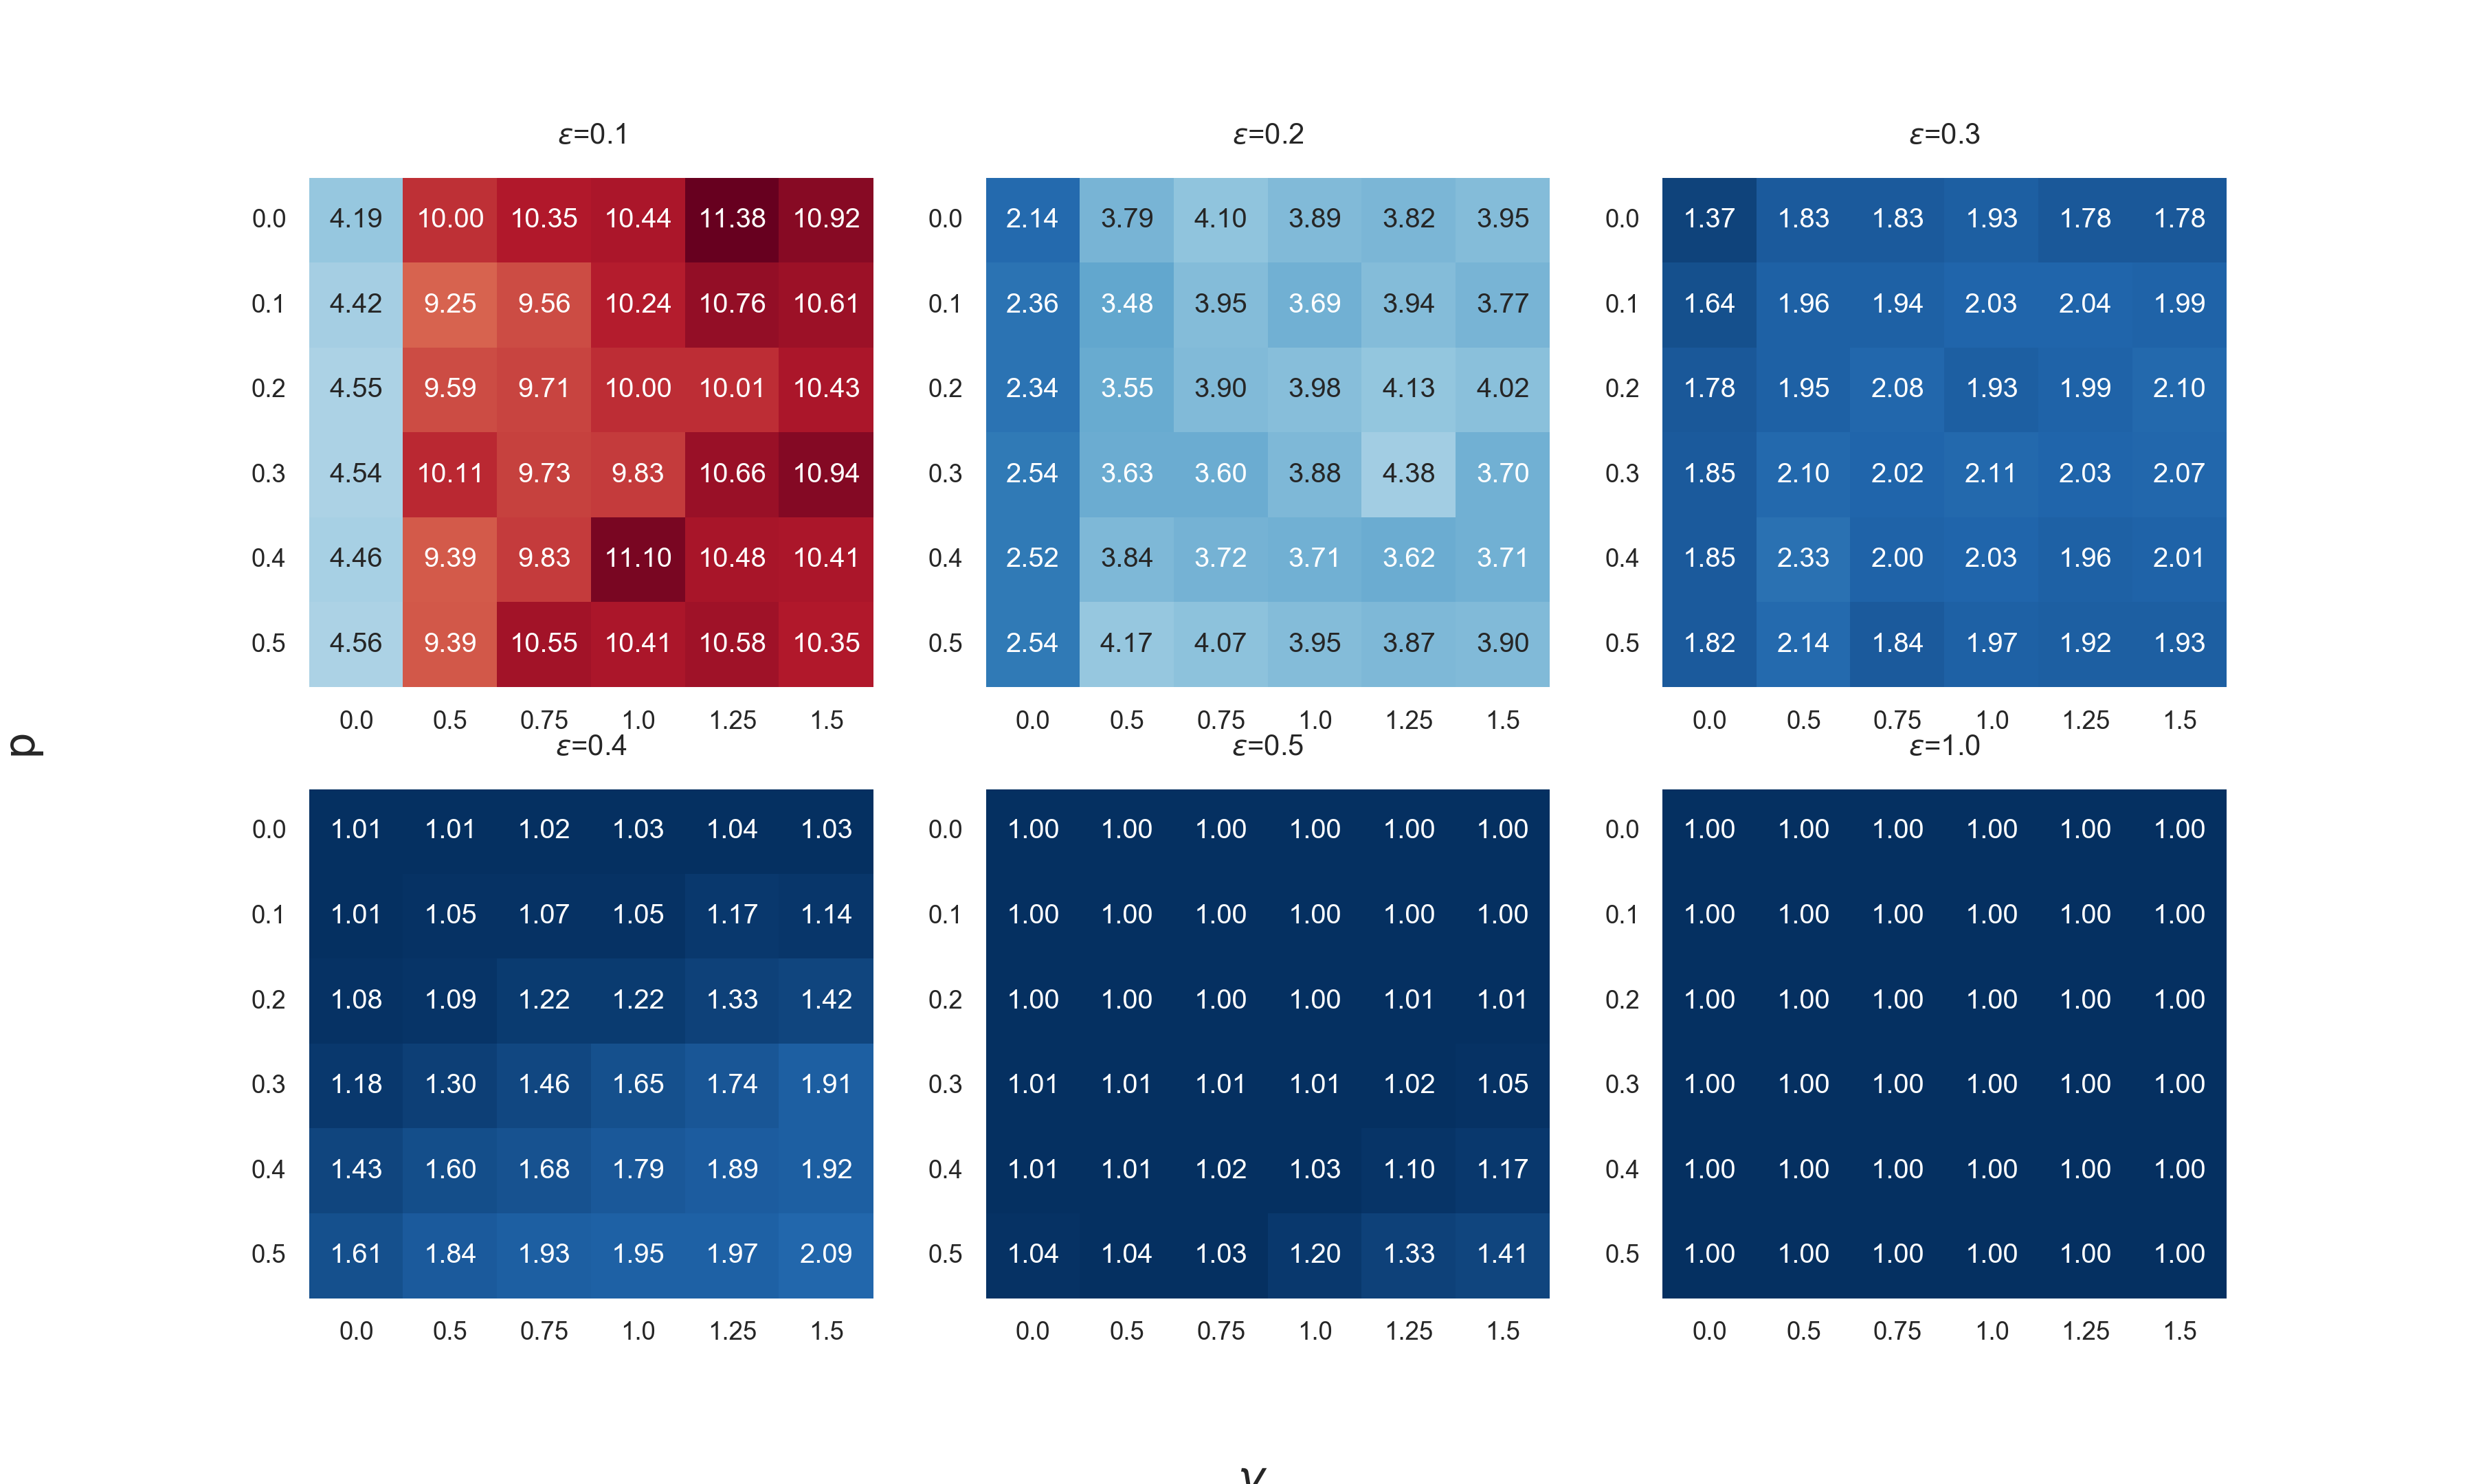
\includegraphics[width = 0.8\textwidth]{figures/hm media mo0.0 0.01MS_avg_ncluster groupedby_eps.png}
    \caption{\textbf{Average number of clusters with one extreme media.} The figure shows the average number of clusters for different values of the confidence bound $\epsilon$ as a function of $\gamma$ and $p_m$.}
    \label{fig:00ncluster}
\end{figure}

In the case we have one extreme media, namely $m_1 = 0.0$ a higher probability of interacting with such media and a higher bias both enhance fragmentation, as we can see from figure \ref{fig:00ncluster}, where the average number of clusters of the final distribution is plotted for different values of the confidence bound $\epsilon$ as a function of $\gamma$ and $p_m$. We can see how, in this case, the number of clusters can grow due to the bias, but also due to a higher number of interactions with a single fixed external source of information, which can radicalise a portion of the population. 
\begin{figure}
    \centering
    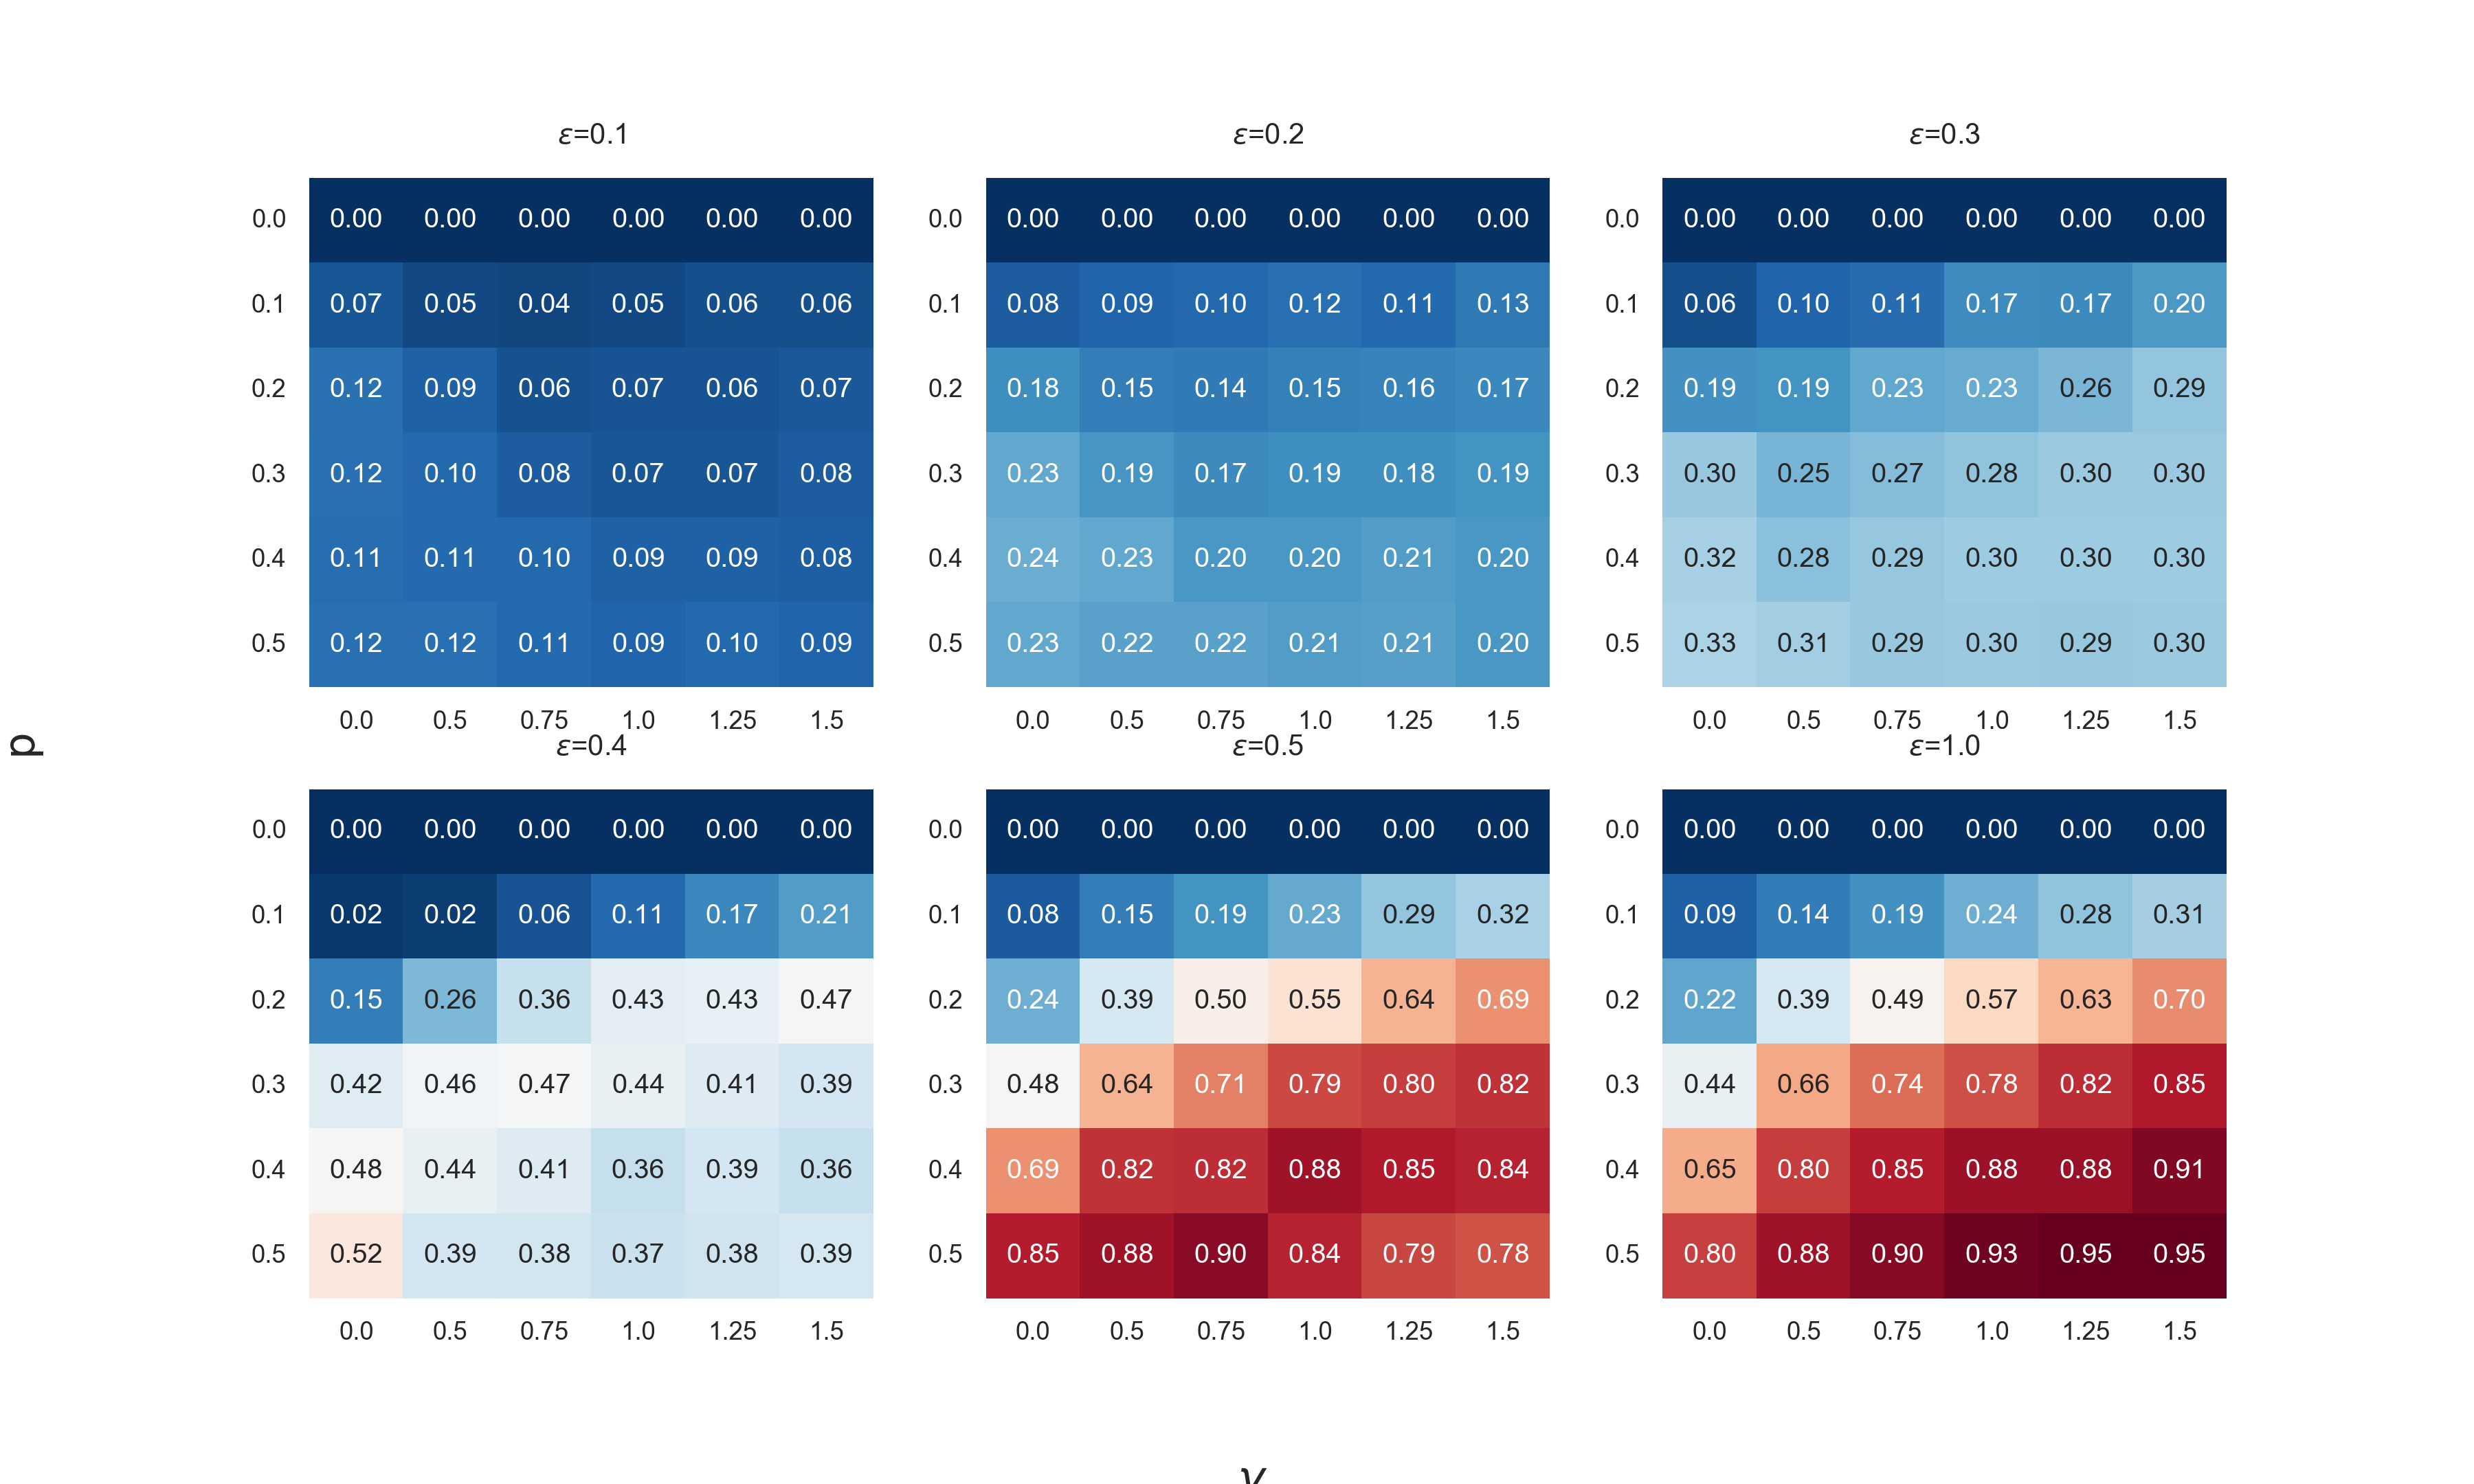
\includegraphics[width=0.8\textwidth]{figures/hm media mo0.0 perc_00 groupedby_eps.png}
    \caption{\textbf{Percentage of nodes in the extremist media cluster.}}
    \label{fig:extrnodes}
\end{figure}
If we consider the percentage of agents that hold opinions in the range $[0.0, 0.0+\lambda]$ we can see from figure \ref{fig:extrnodes} that this percentage is already around $20-30\%$ with a probability to interact with the media of only $10\%$. Moreover, while a high confidence bound can restore consensus, the mean opinion tends towards 0 until there is a full consensus around the extreme opinion for very high $\epsilon$ values and $p_m$ values. In this case, a higher bias means still a higher fragmentation, but it also means that a small part of the population can separate themselves from the extremist consensus. The presence of one single media agent also fastens the convergence (the number of iterations at convergence slightly reduces as $p_m$ grows) whether the final state is fragmented, polarised or a consensus and - differently from the baseline AB model - the presence of an algorithmic bias does not seem to slow down the convergence in a significant way. \\ \\


\textbf{Three media}
\begin{figure}
    \centering
    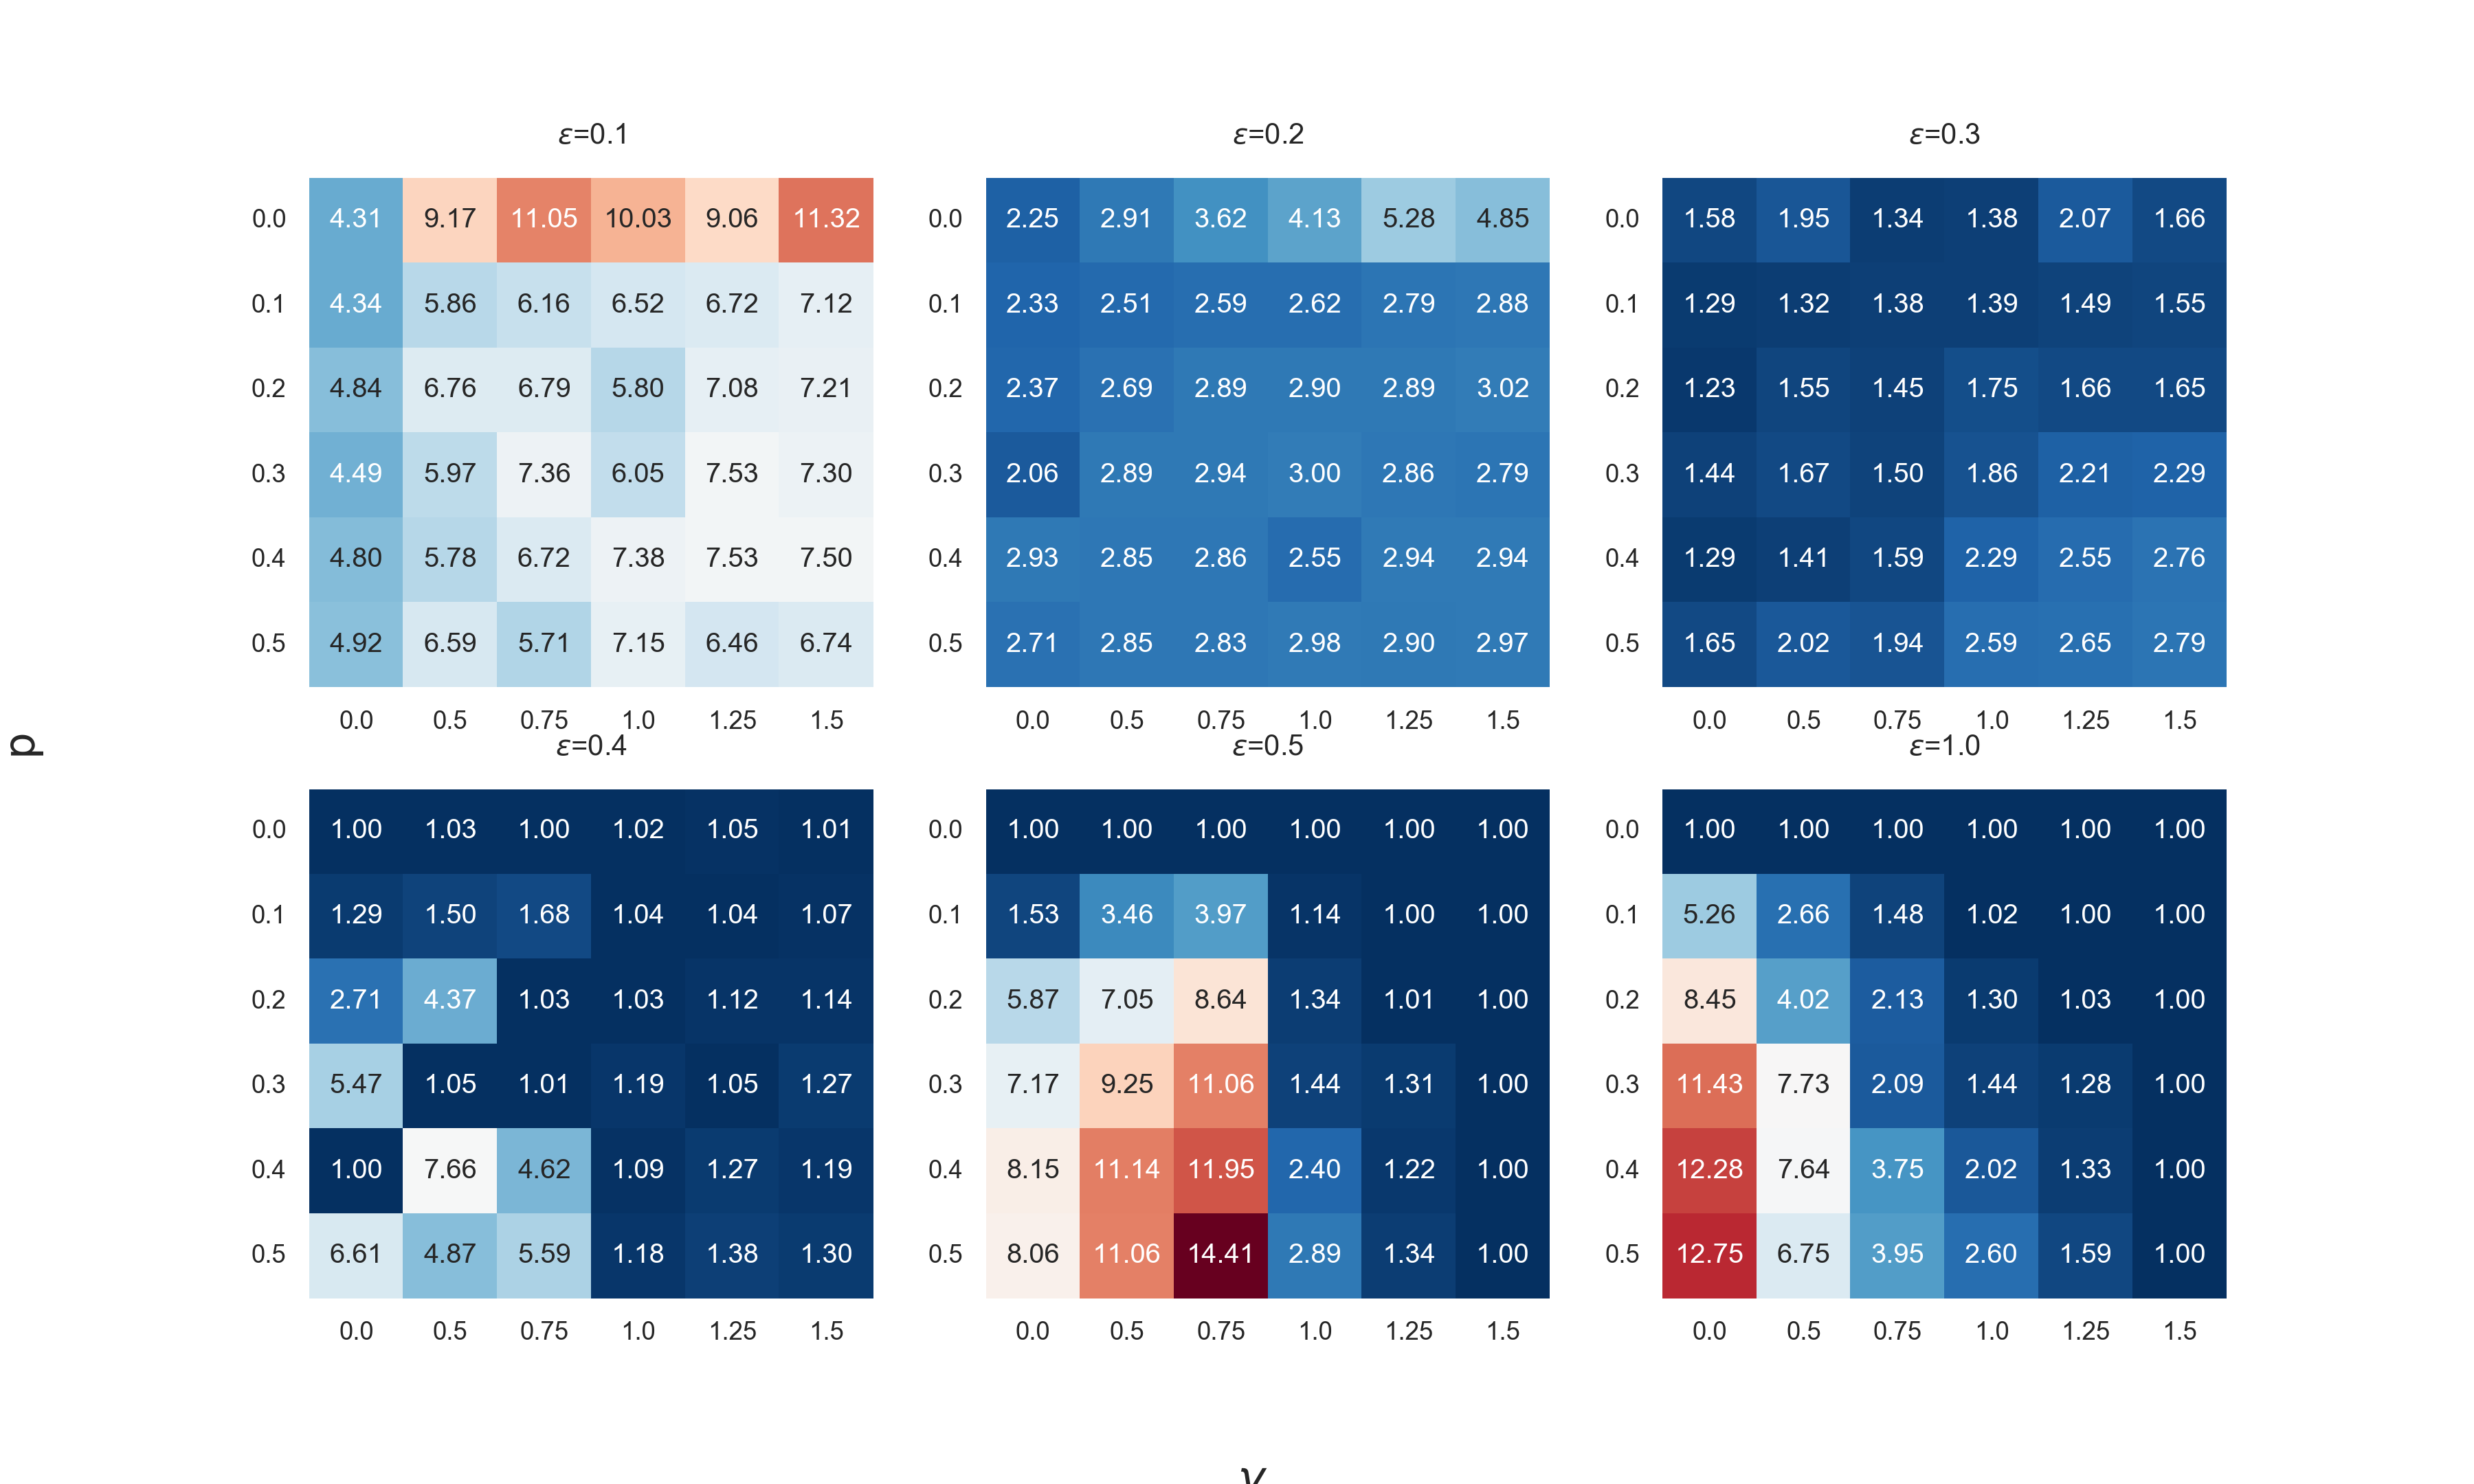
\includegraphics[width=0.8\textwidth]{figures/hm media mo0.05;0.5;0.95 0.01MS_avg_ncluster groupedby_eps.png}
    \caption{\textbf{Average number of clusters for different values of $\epsilon$}}
    \label{fig:3mncluster}
\end{figure}
% \begin{figure}
%     \centering
%     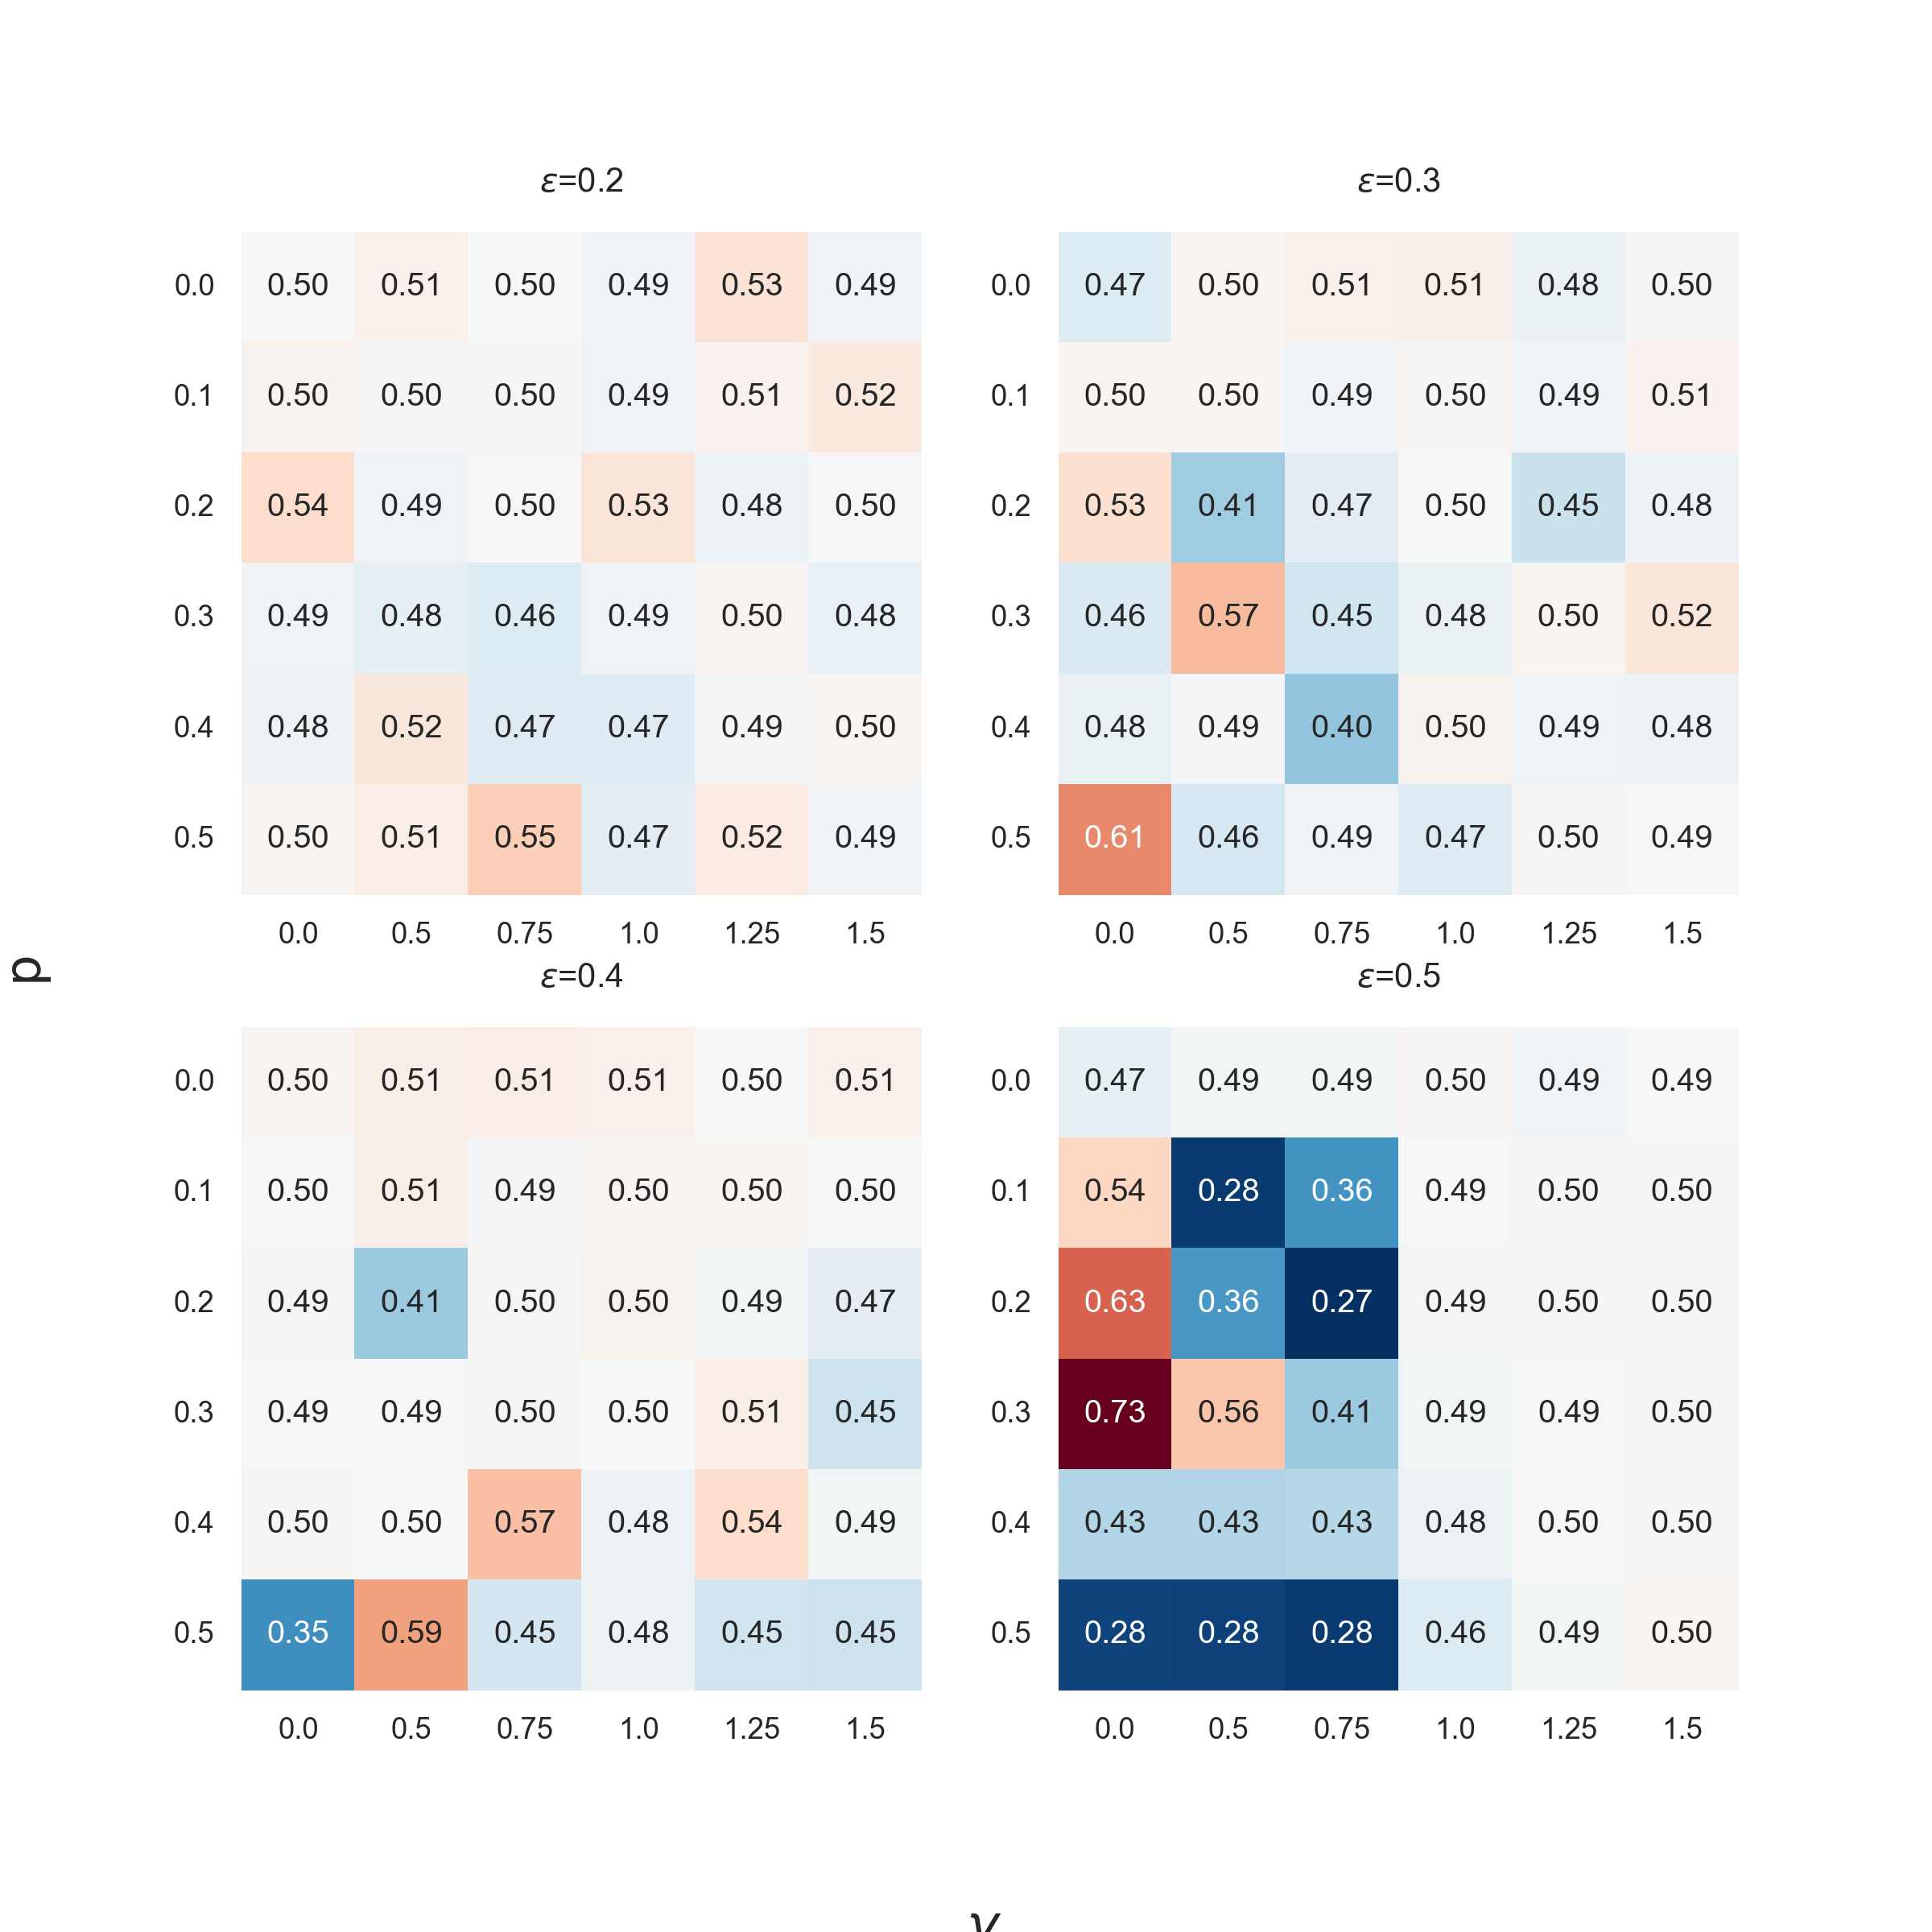
\includegraphics[width=0.8\textwidth]{figures/hm media mo0.05;0.5;0.95 avg_opinion groupedby_eps.png}
%     \caption{\textbf{Average mean opinion.}}
%     \label{fig:3maverageop}
% \end{figure}
Adding multiple media outlets has different results on the outcomes of the opinion dynamics. Since active interactions can happen only with agents within one's confidence bound, for $\epsilon \leq 0.3$ - since media have a $0.45$ distance between them - the dynamics follows the baseline model behaviour: fragmentation increases with both $p_m$ and $\gamma$, but this increase is not substantial: as we can see from \ref{fig:3mncluster} we go from two to three clusters for $\epsilon=0.2$ and from 1 to 3 clusters for $\epsilon=0.3$. Moreover, 
% as we can see from figure \ref{fig:3maverageop} 
agents tend to cluster around the media opinions, so the media \say{attract} the population and rapidly fragments them. When $\epsilon \geq 0.4$, however, an increase in $p_m$ enhances fragmentation: agents remain sparser in the opinion spectrum, distributing themselves between the opinions of two media and - in some cases - maintaining a uniform distribution between 0.05 and 0.95; moreover, fragmentation is also enhanced by a substantial slowing down in convergence, or, more precisely, the absence of convergence, since nodes keep on interacting with different fixed opinions - the media ones - and with these interactions being active they keep shifting their position in the opinion spectrum, enhancing instability of the system; the mean opinion at the end of the dynamics is very variable, while in all other cases it's pretty stable around 0.5, and it depends on the fact that sometimes all the agents are attracted in the space between 0.05 and 0.5, while in other cases they are attracted between 0.5 and 0.95, while in others they converge in a few clusters. This different final state is visible also by comparing the average number of clusters with the average pairwise distance. While in the baseline model the number of clusters and the pairwise distances followed the same behaviour, in this case, we have a very high number of clusters with an extremely low pairwise distance because agents are closer to each other than in a polarised situation. Still, their distribution has much higher entropy, i.e., number of clusters. Perhaps counterintuitively, if we also increase $\gamma$ - while increasing the probability to interact with media - this reduces the level of fragmentation in the system and brings it to consensus around the mean opinion (0.5), as we can see from the percentage of nodes in $[0.5-\lambda, 0.5+\lambda]$.
\section{Conclusions}
\label{sec:conlcusion}
A bounded confidence model with algorithmic bias and mass media agents was presented. We found that the presence of one extremist media can always radicalise a portion of the population, depending on the probability of interacting with this media and the filtering power of the algorithm. A higher number of media interactions brings a higher percentage of the population towards the extreme, while increasing the filtering power of the algorithm fragments the population and reduces the number of final extremists, since it makes it less probable for the agents on the opposite side of the opinion spectrum to interact with the media at all. When the number of media in the system is higher than one, this can highly change the dynamics: in the case of a low \say{open-mindedness} - i.e. $\epsilon \leq 0.3$ the population clusters around the media opinions on average, while for $\epsilon > 0.3$, the dynamics are volatile up to a specific value of $\gamma$, because agents keep on changing their opinions due to the agent-to-media interactions, while a strong filtering power enhances consensus, when combined with a high probability of agent-to-media interactions. 

\bibliography{references}

\section{Supplementary Materials}
\begin{figure}
    \centering
    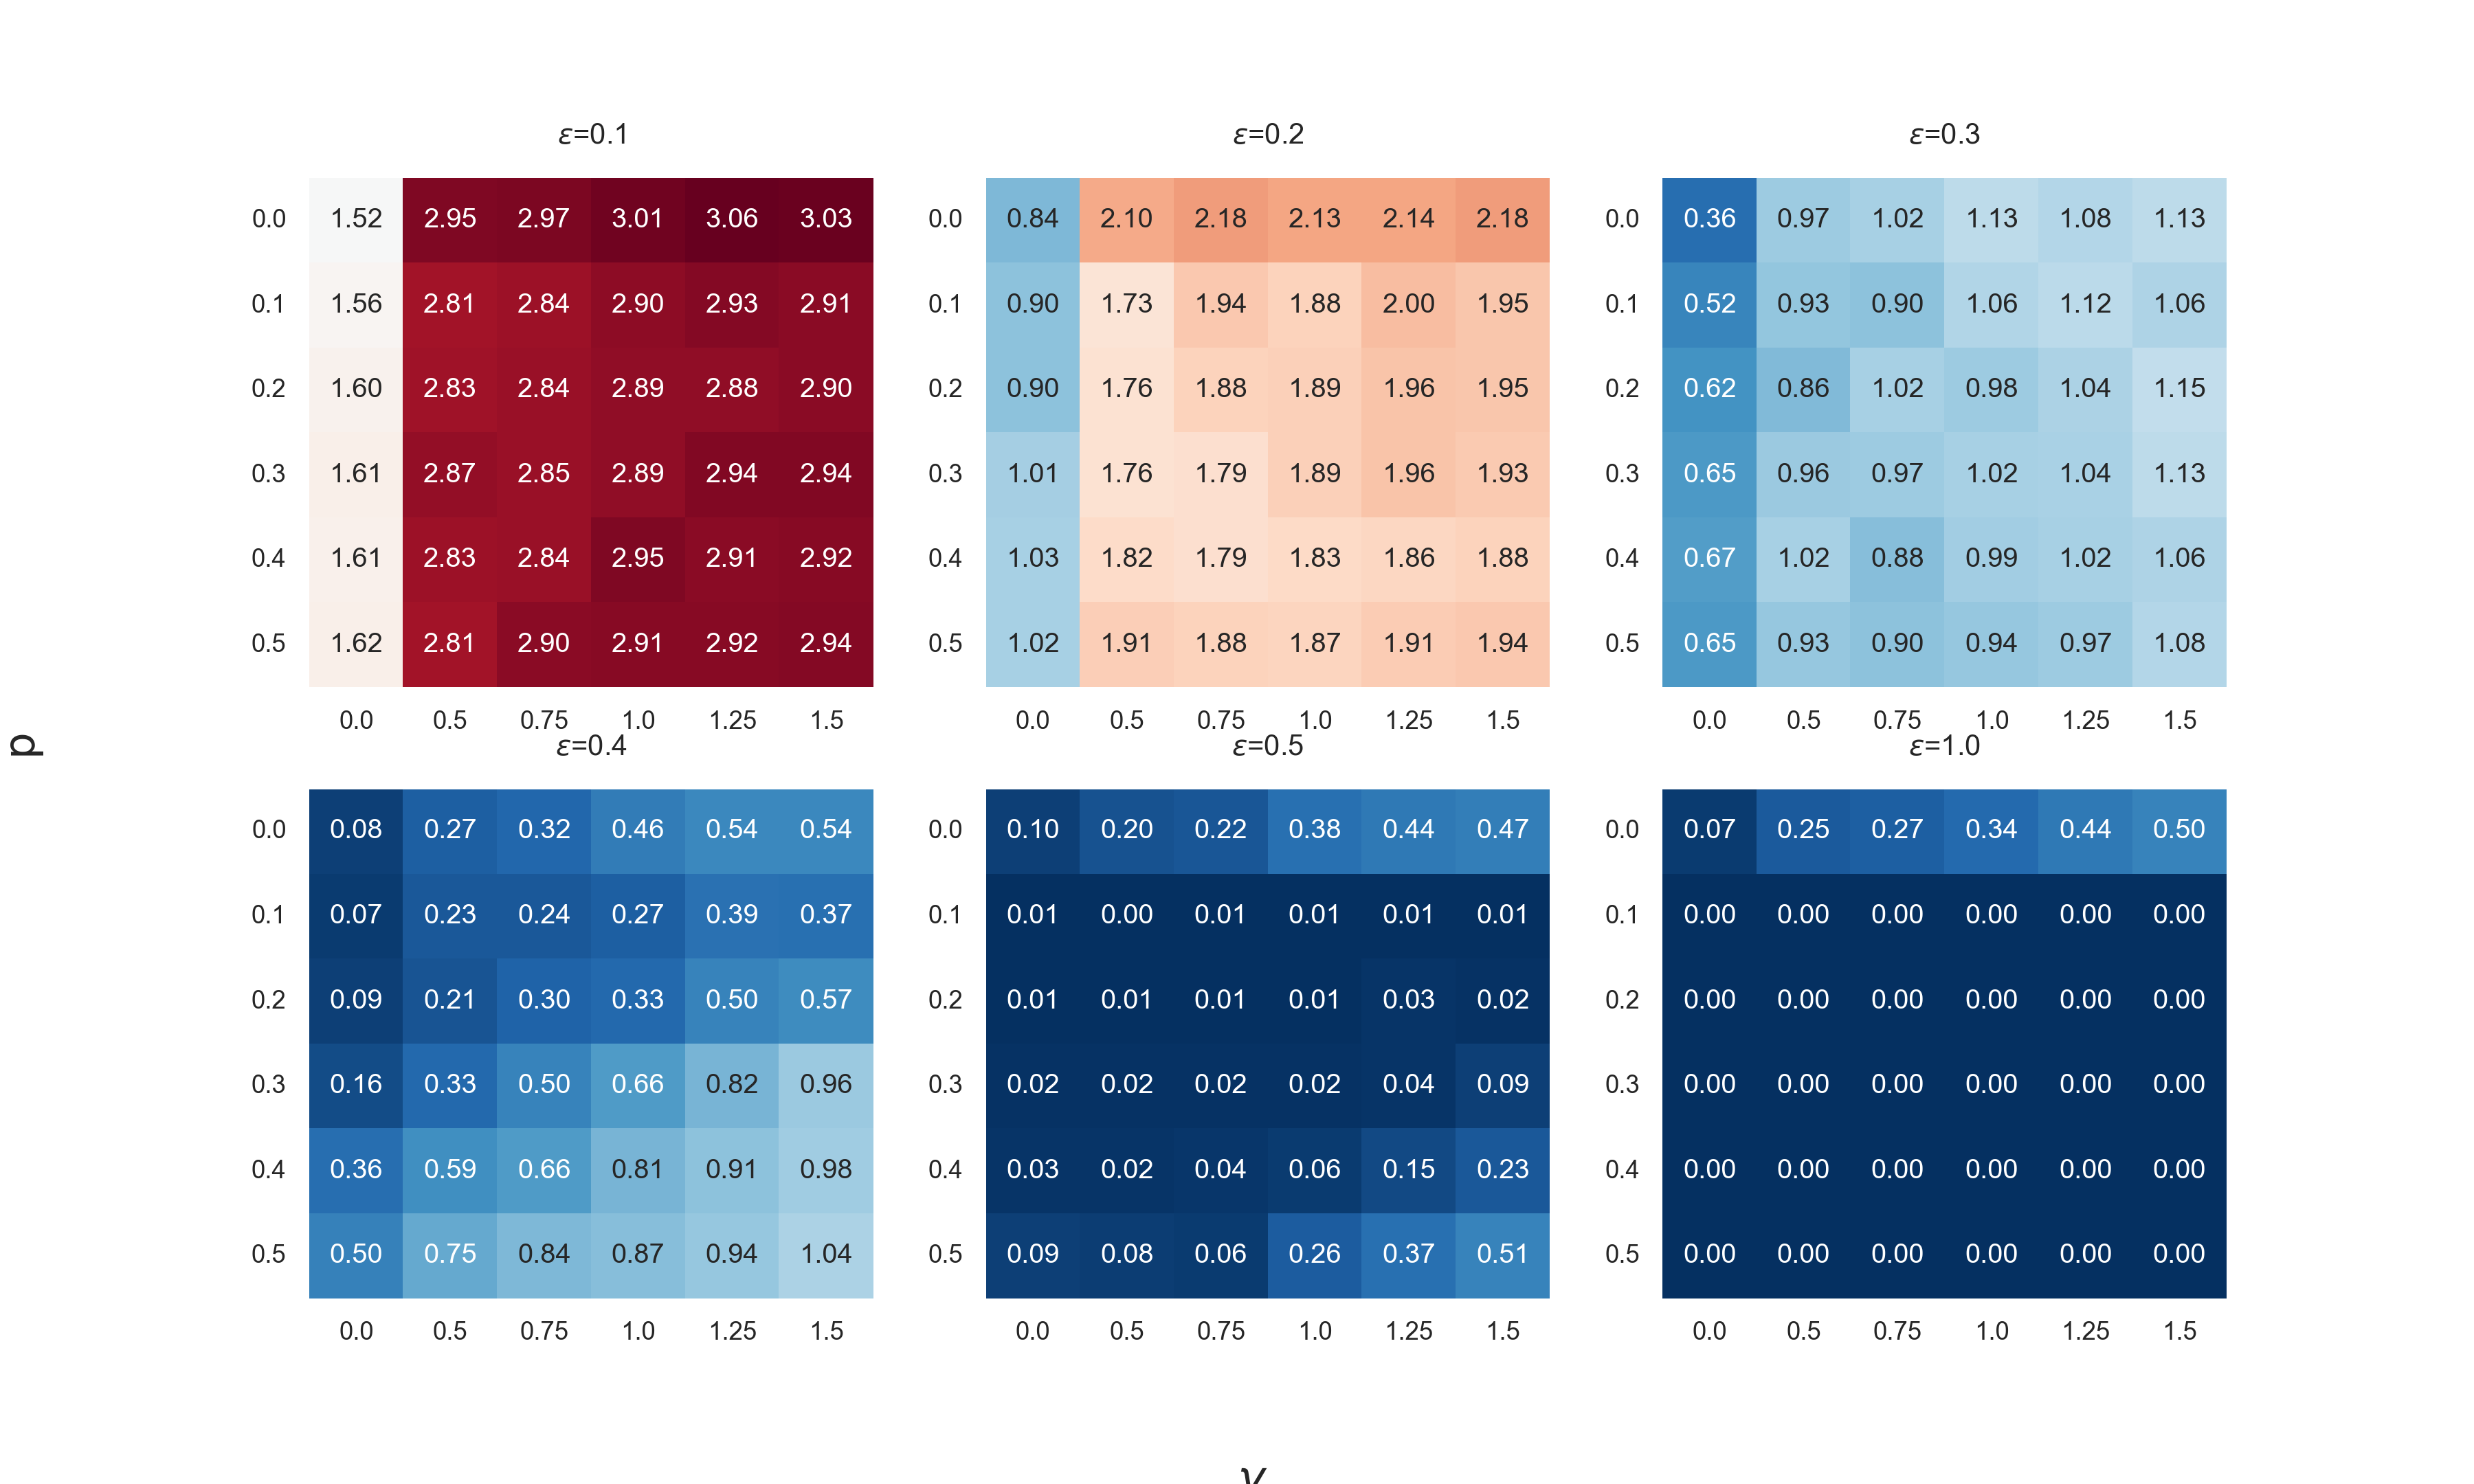
\includegraphics{figures/hm media mo0.0 10B_avg_entr groupedby_eps.png} 
    \caption{\textbf{Average entropy of final opinion distribution with one media with opinion equal to 0.0.} The figure shows the average entropy of the discrete probability distribution of a node $i$ to be in one of the 10 intervals $k$ of width $0.1$, $p(k)$. As we can see, the behaviour of the average entropy is very similar to the behaviour of the average number of clusters, since they both capture how fragmented or disordered is the final distribution. The heatmaps show how for $\epsilon=0.2$ without biasing the interactions the entropy goes from $0.84$ to $1.02$ as the probability to interact with the media increases, but is always higher for $p_m=0.0$ if we have a bias $\gamma > 0$. In the case of $\epsilon =0.3$ entropy grows with $p_m$ with $\gamma=0.0$, while we have around the same level of entropy when there is a higher bias for every value of $p_m$. In the case of $\epsilon=0.4$ we can see how the average entropy grows both with $p_m$ and with $\gamma$ going from values around $0$ if the parameters are both null, to around $1$ if the parameters grow. In the last case presented in this figure, $\epsilon=0.5$, we can see that the average entropy is much lower than the other cases, going from $0$ to $0.5$ at most. However we can still see that it grows both with $p_m$ and with $\gamma$.}
    \label{fig:00avg10Bentrbyeps}
\end{figure}

\begin{figure}
    \centering
    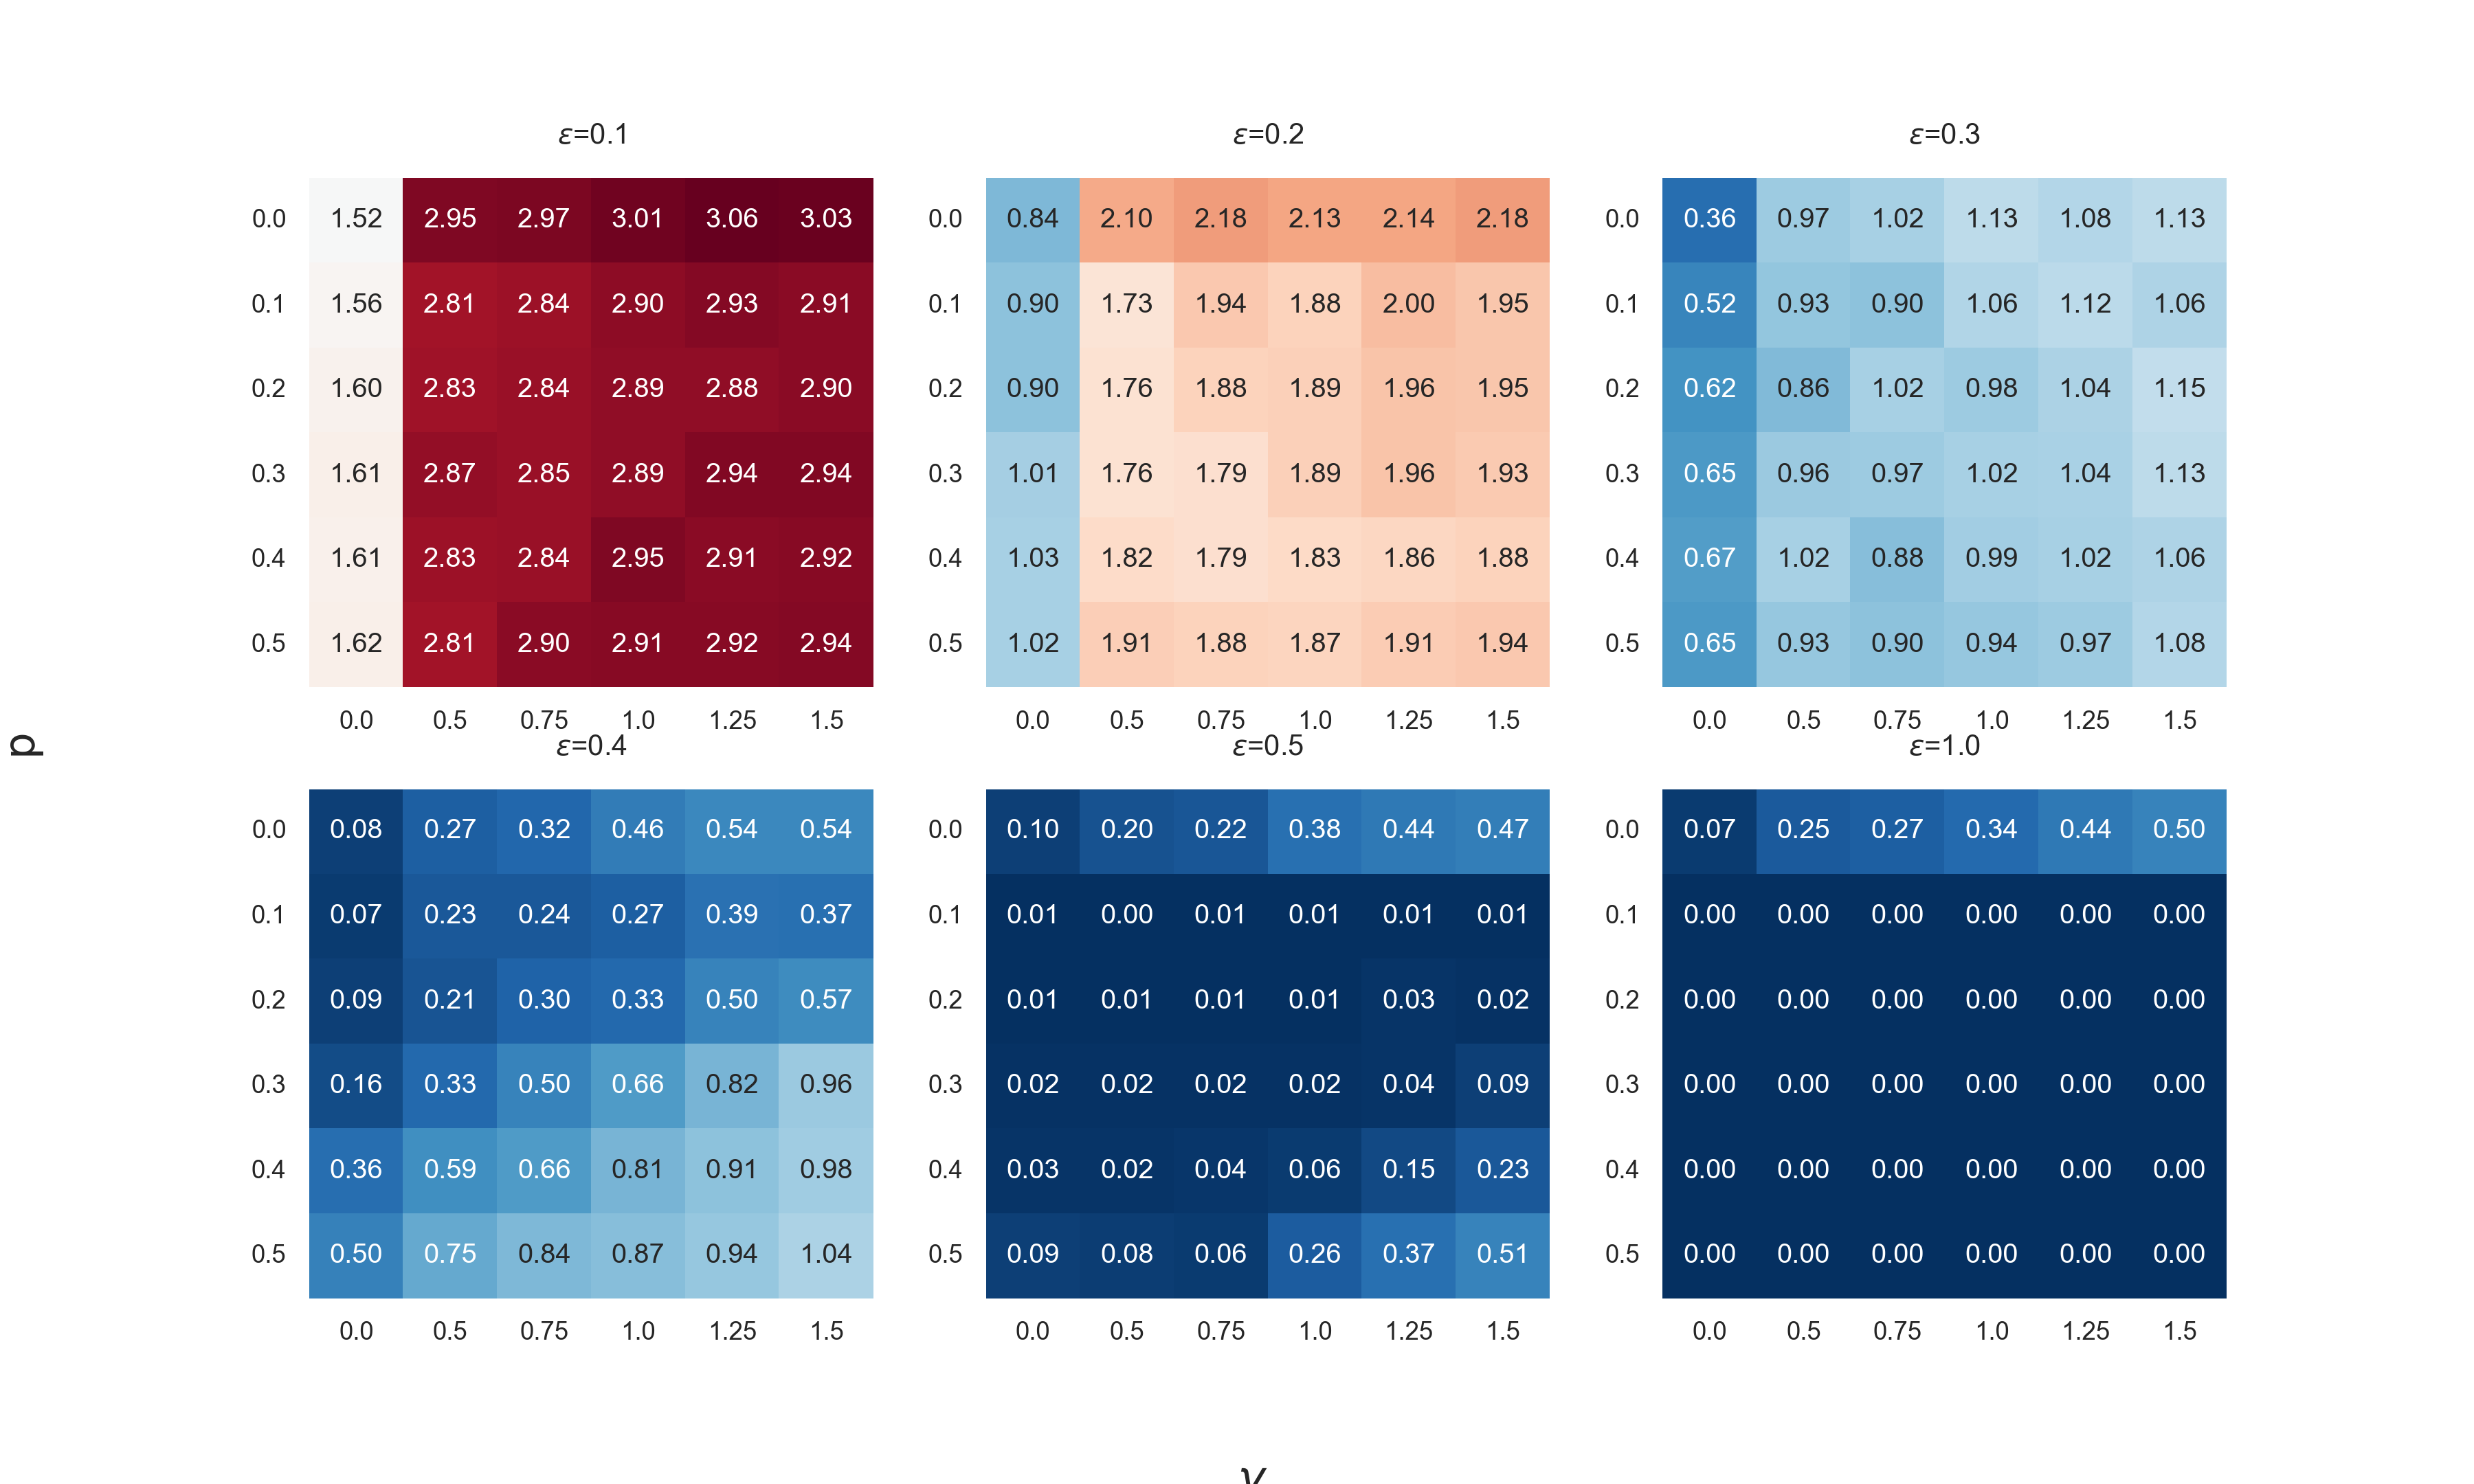
\includegraphics{figures/hm media mo0.0 100B_avg_entr groupedby_eps.png}
    \caption{\textbf{Average entropy of final opinion distribution with one media with opinion equal to 0.0.} In this case the average entropy was computed using a discrete probability distribution obtained by binning the final distribution in 100 bins of equal width. As we can see, the values are consistent with the 10 bins case.}
    \label{fig:00avg100Bentrbyeps}
\end{figure}

\begin{figure}
    \centering
    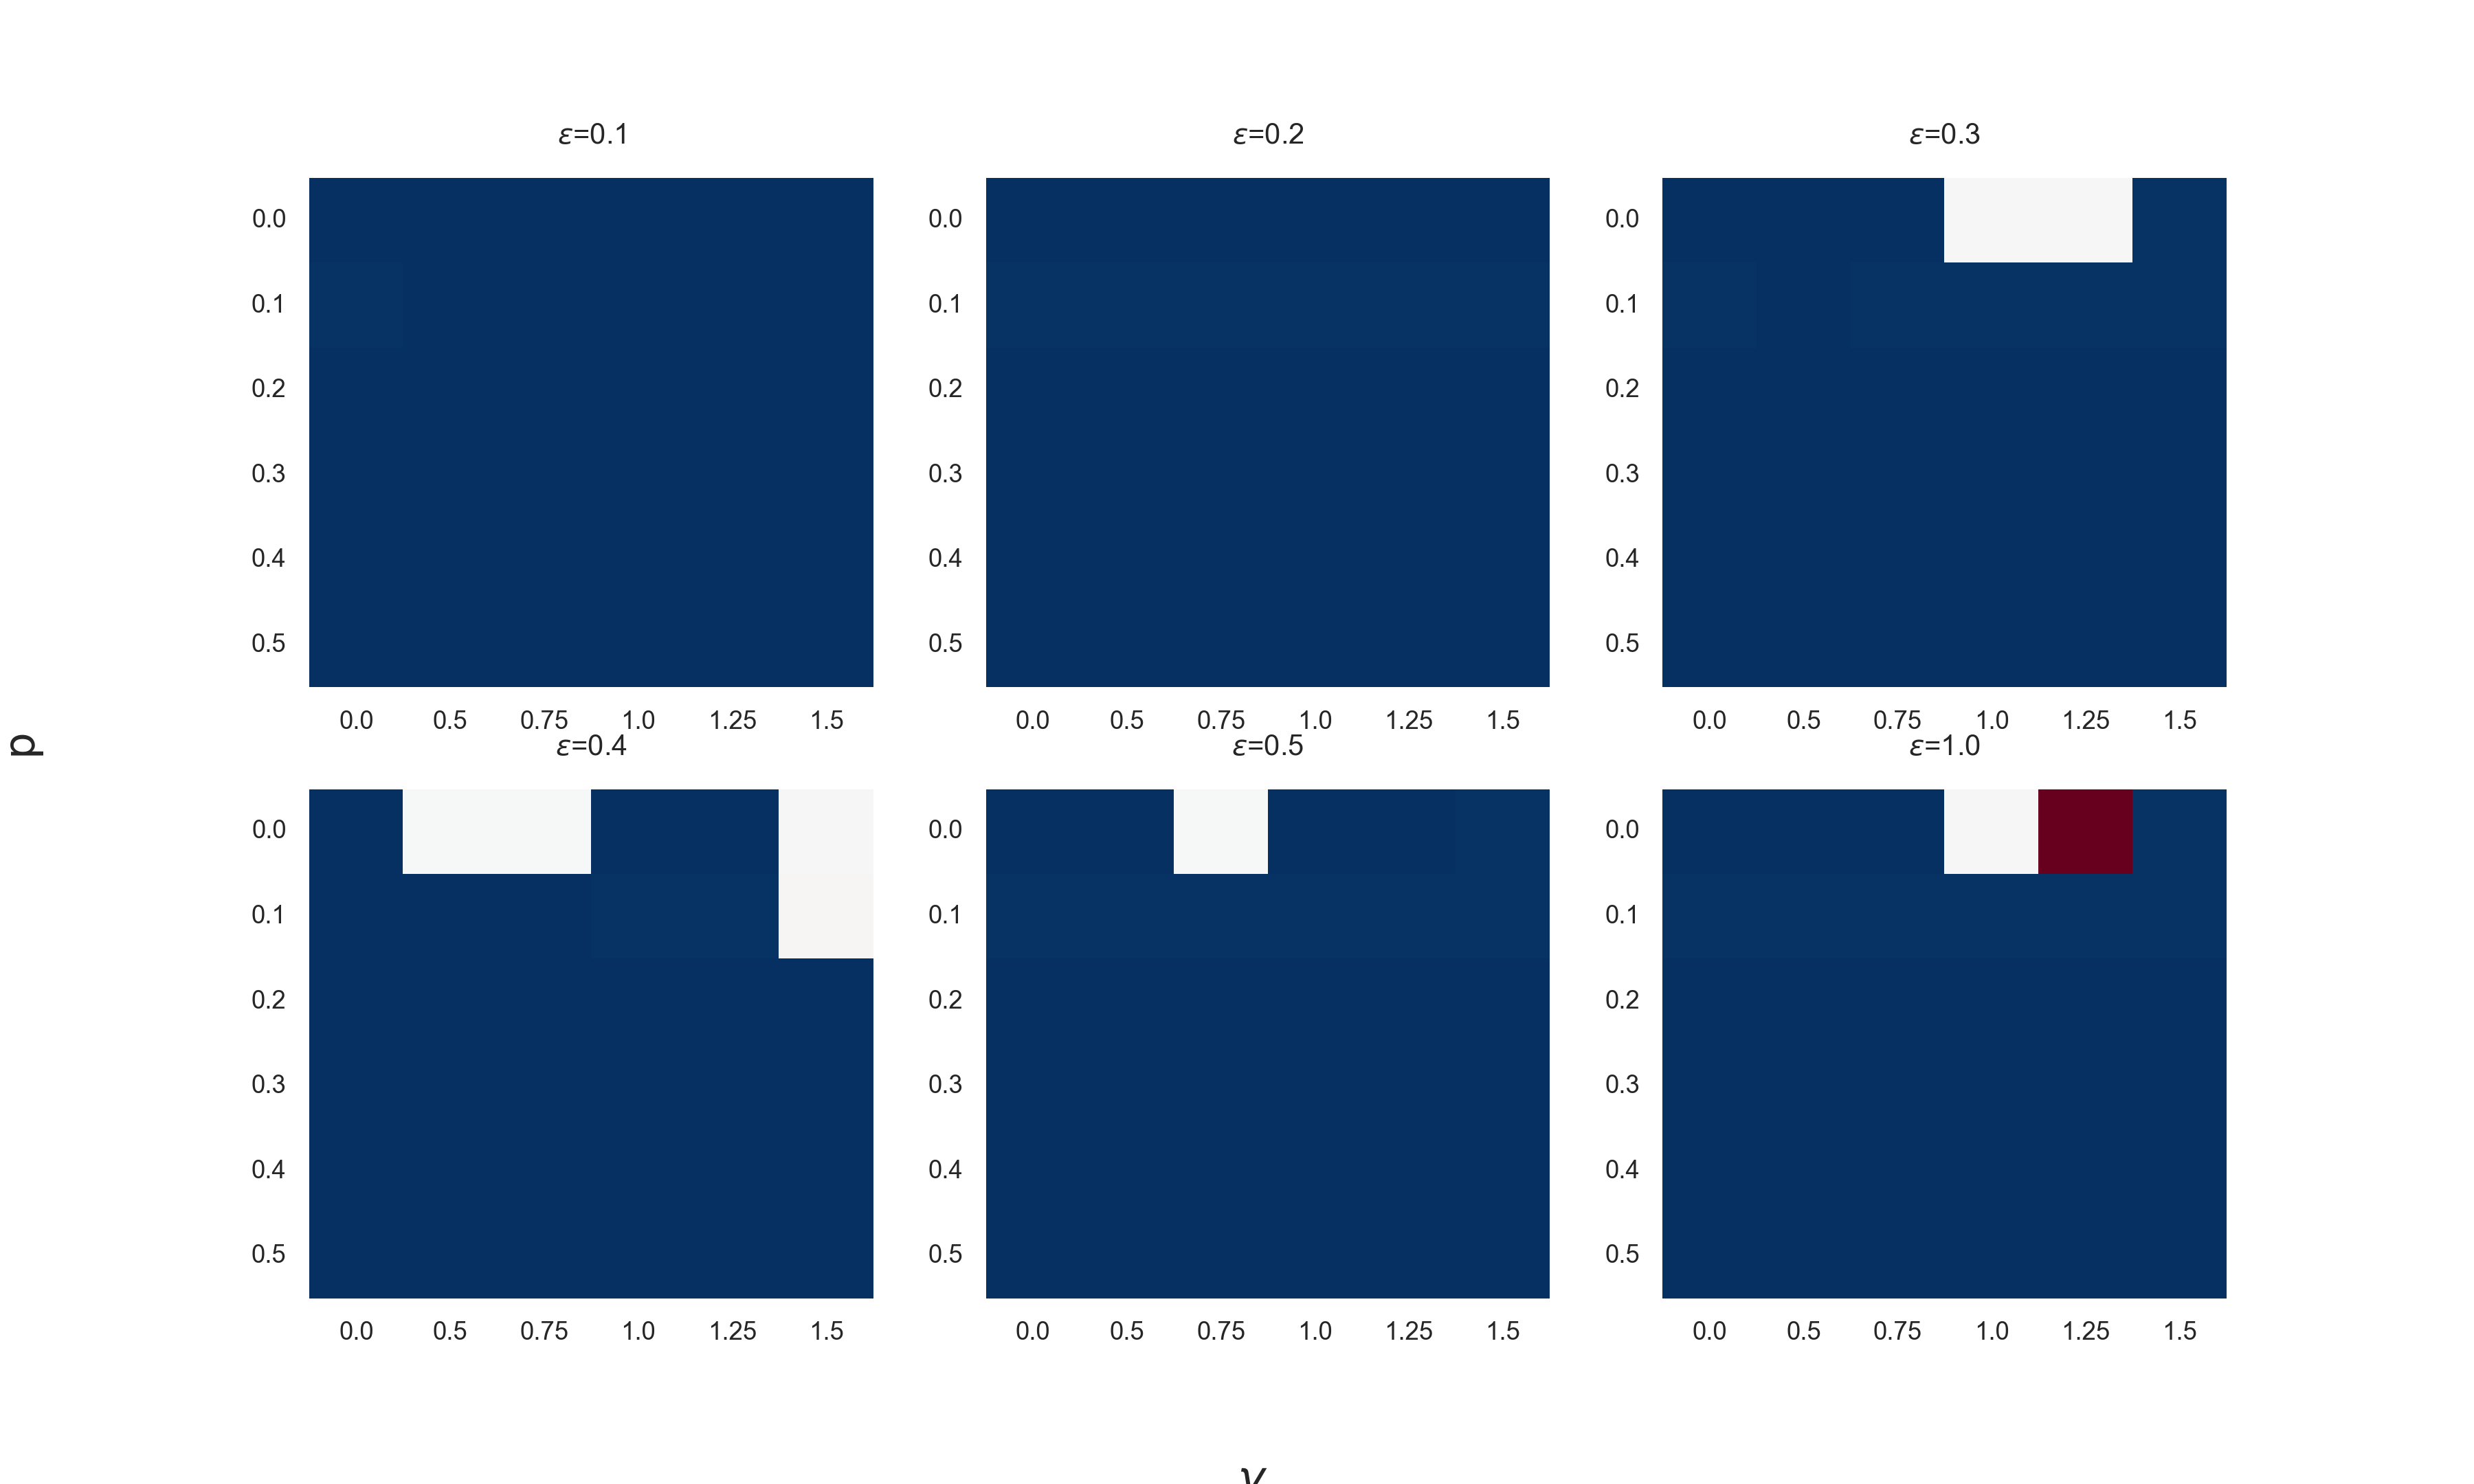
\includegraphics{figures/hm media mo0.0 avg_niter groupedby_eps.png}
    \caption{\textbf{Average number of interactions to convergence in the case of one extreme media for different values of $\epsilon$ as a function of $\gamma$ and $p_m$.} As we can see convergence is rather fast and only slightly increases with $\gamma$. There are only a few cases where convergence is very slow, when the probability to interact with the media is low and $\gamma > 0$. }
    \label{fig:00avgniterbyeps}
\end{figure}

\begin{figure}
    \centering
    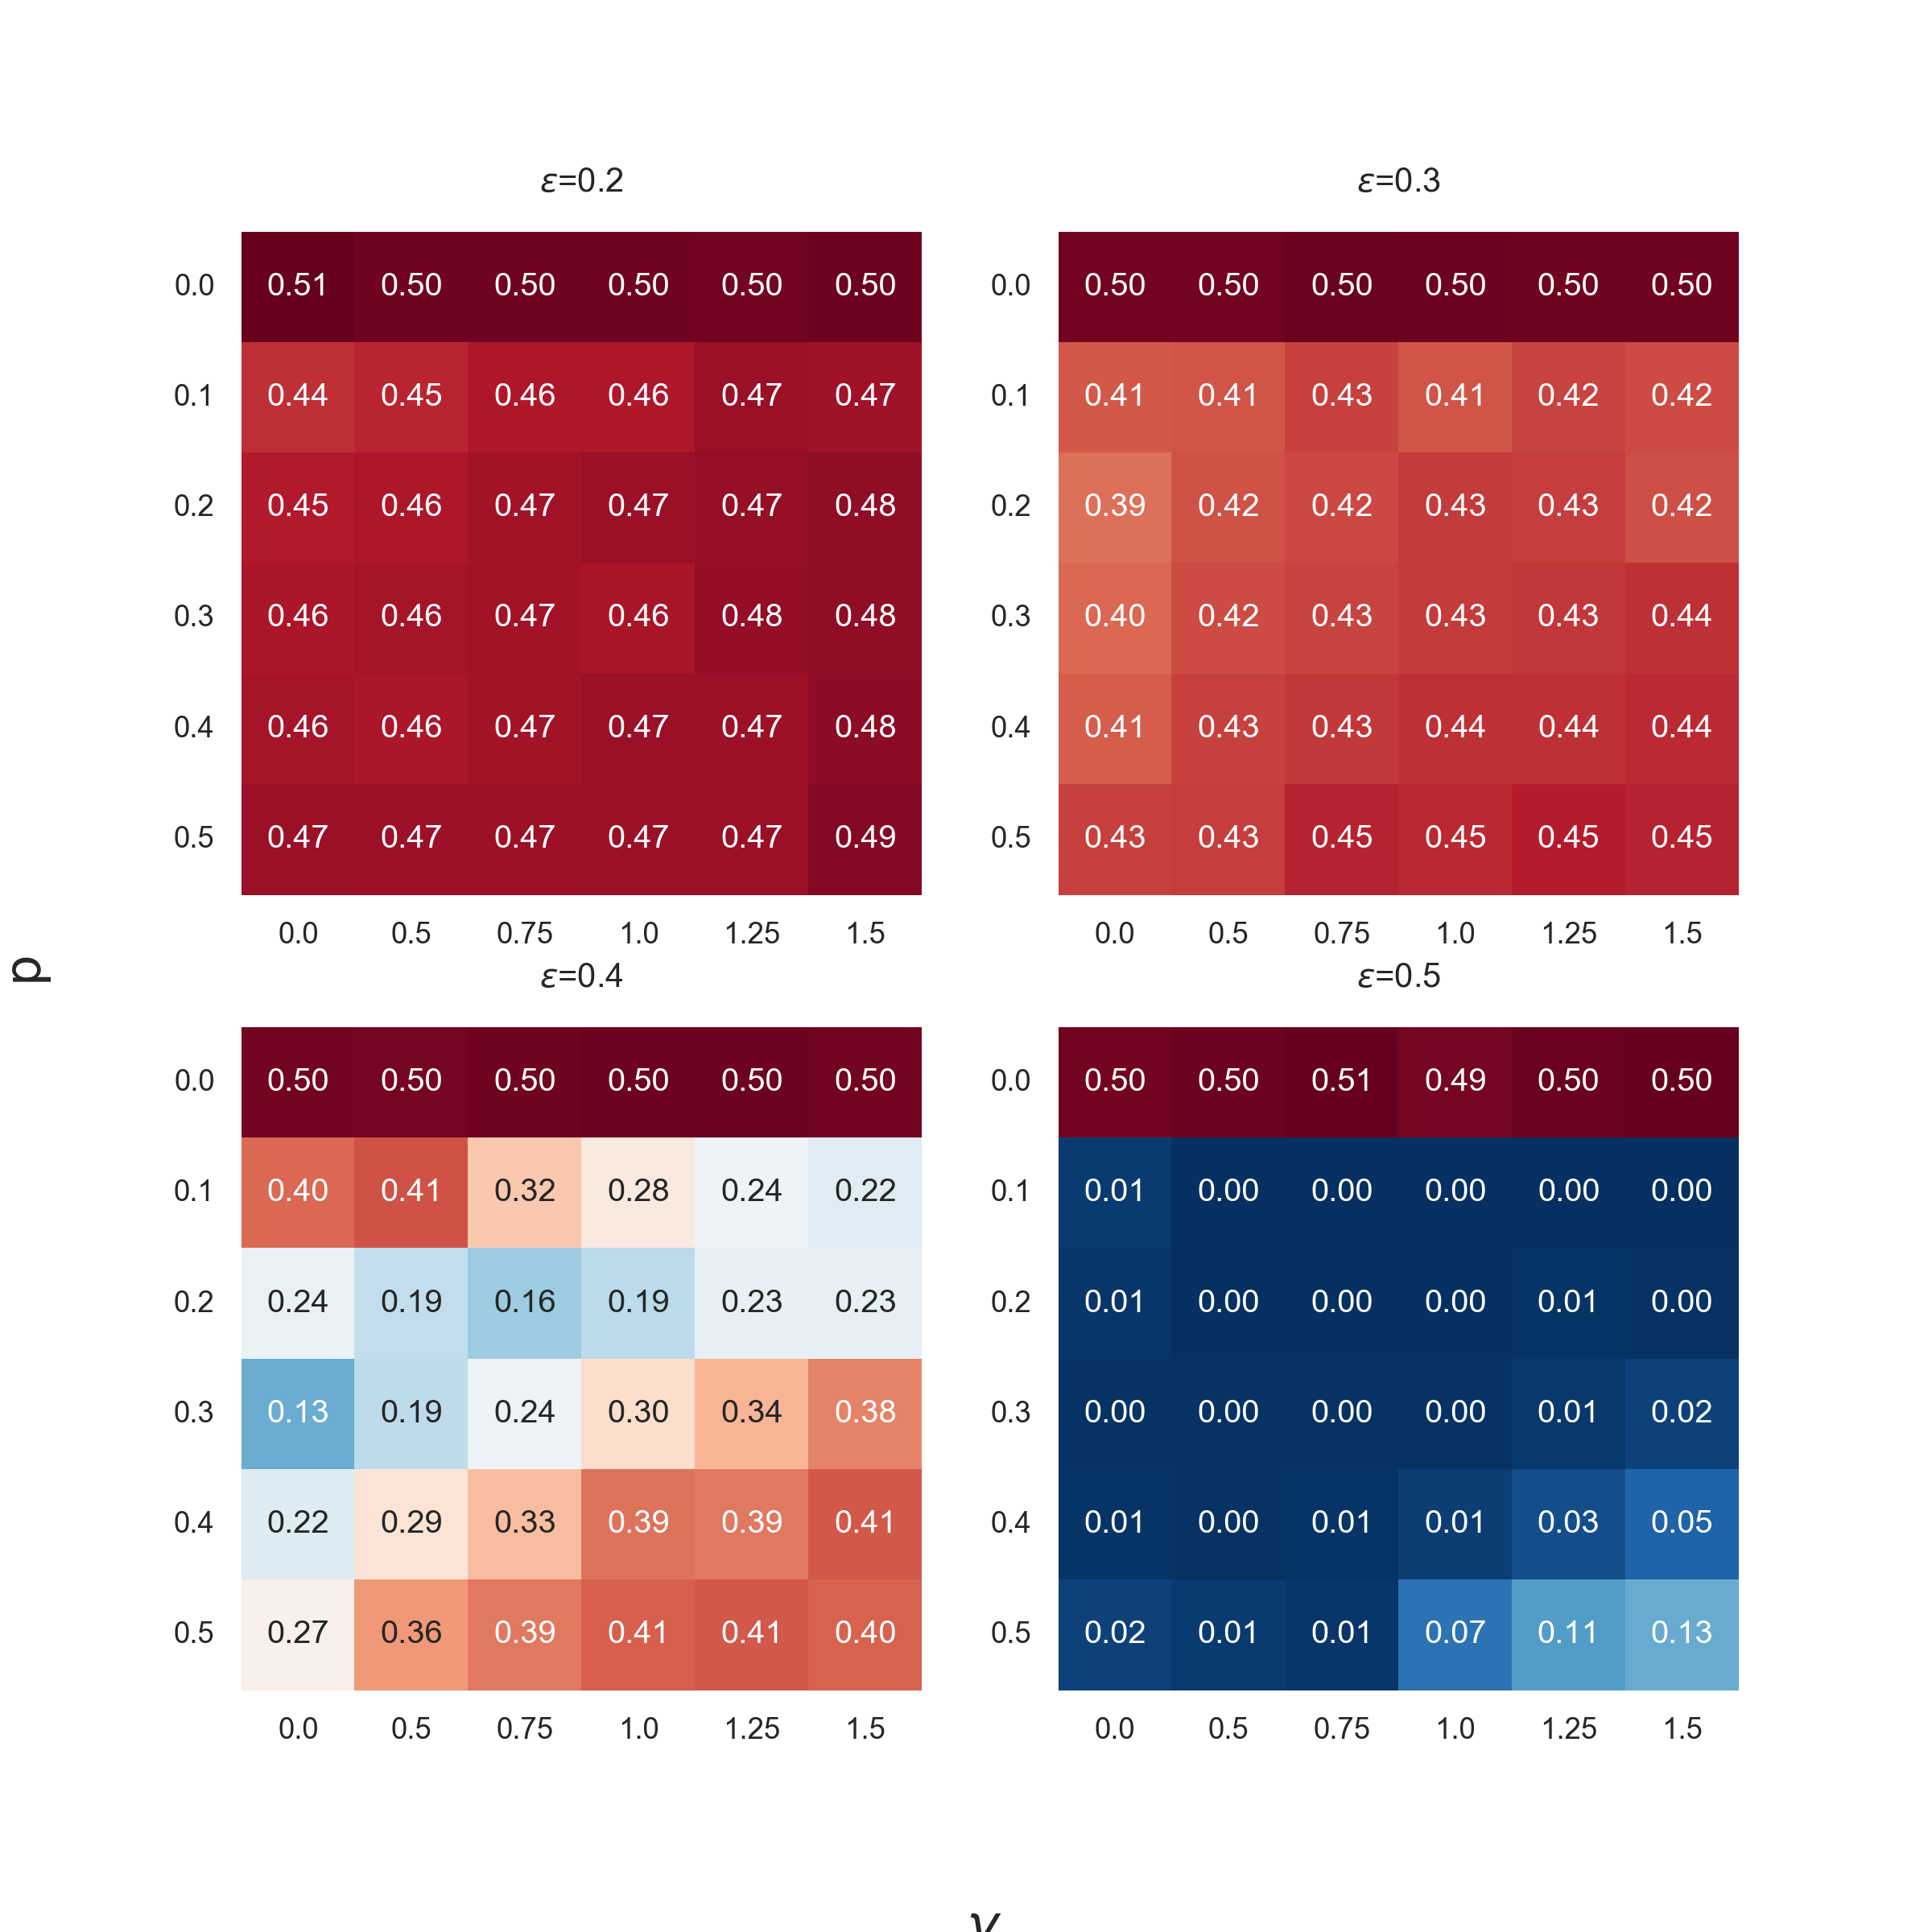
\includegraphics{figures/hm media mo0.0 avg_opinion groupedby_eps.png}
    \caption{\textbf{Average final opinion in the case of one extreme media for different values of $\epsilon$ as a function of $\gamma$ and $p_m$.} We can see from the figure that in the case of no interactions with the media the average opinion is always around $0.5$, meaning that when there is consensus nodes converge to the central opinion and when there are 2 or 3 clusters, these cluster are of similar sizes and in opposite parts of the opinion spectrum. However, adding media interactions we can see that, as $p_m$ grows, the average opinion moves towards $0.0$ and s $\gamma$ grows the average opinion slightly grows again. This is probably because when $\gamma$ is high, some nodes don't interact with the media due to the algorithmic bias and therefore don't end up in the \say{extremists} cluster. For $\epslion = 0.5$ there is always full consensus around $0$ for $p_m > 0$.}
    \label{fig:00avgopinionbyeps}
\end{figure}

\begin{figure}
    \centering
    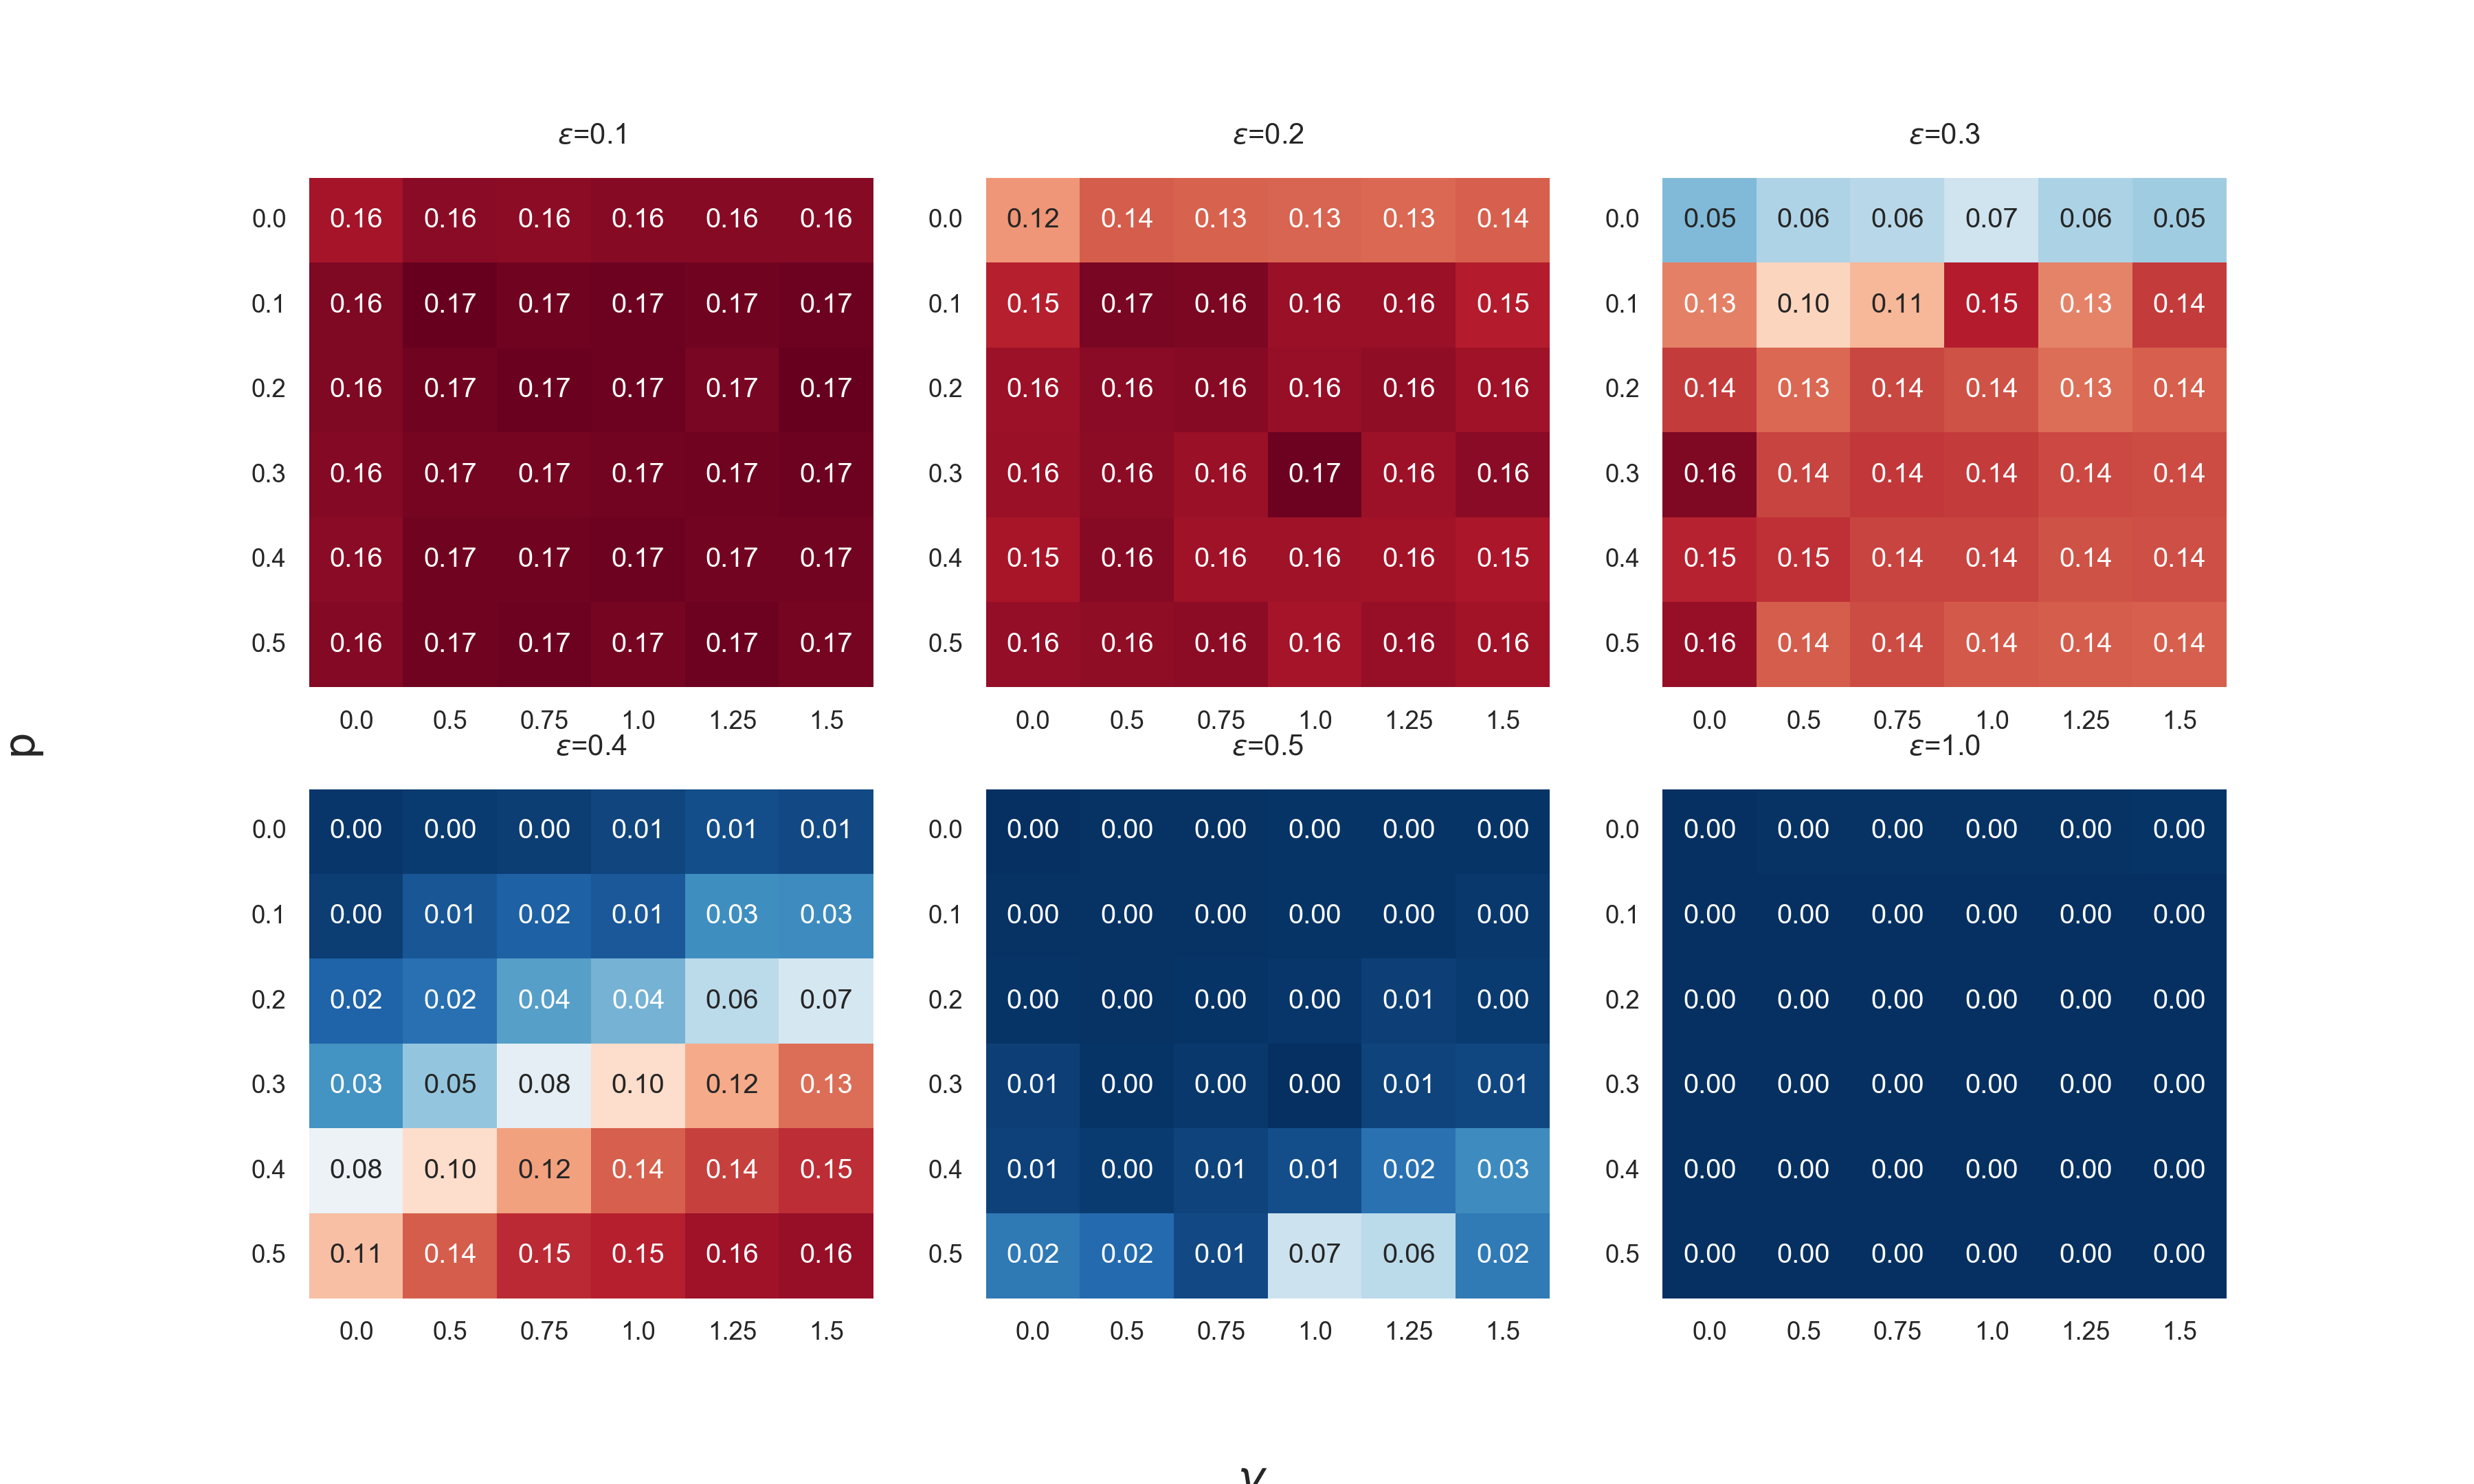
\includegraphics{figures/hm media mo0.0 avg_pwdist groupedby_eps.png}
    \caption{\textbf{Average pairwise opinion distance in the case of one extreme media for different values of $\epsilon$ as a function of $\gamma$ and $p_m$.} We can see that the average pairwise distance when there are no interactions with media is lower and close to $0$ for $\epsilon \geq 0.3$. In the case of $\epsilon \geq 0.4$ we can see how the average pairwise opinion distance follows the same pattern as the average number of clusters and the average entropy, growing both with $p_m$ and $\gamma$. It is always between $0.14-0.17$ for $\epsilon < 0.4$.}
    \label{fig:00avgpwdistbyeps}
\end{figure}

\begin{figure}
    \centering
    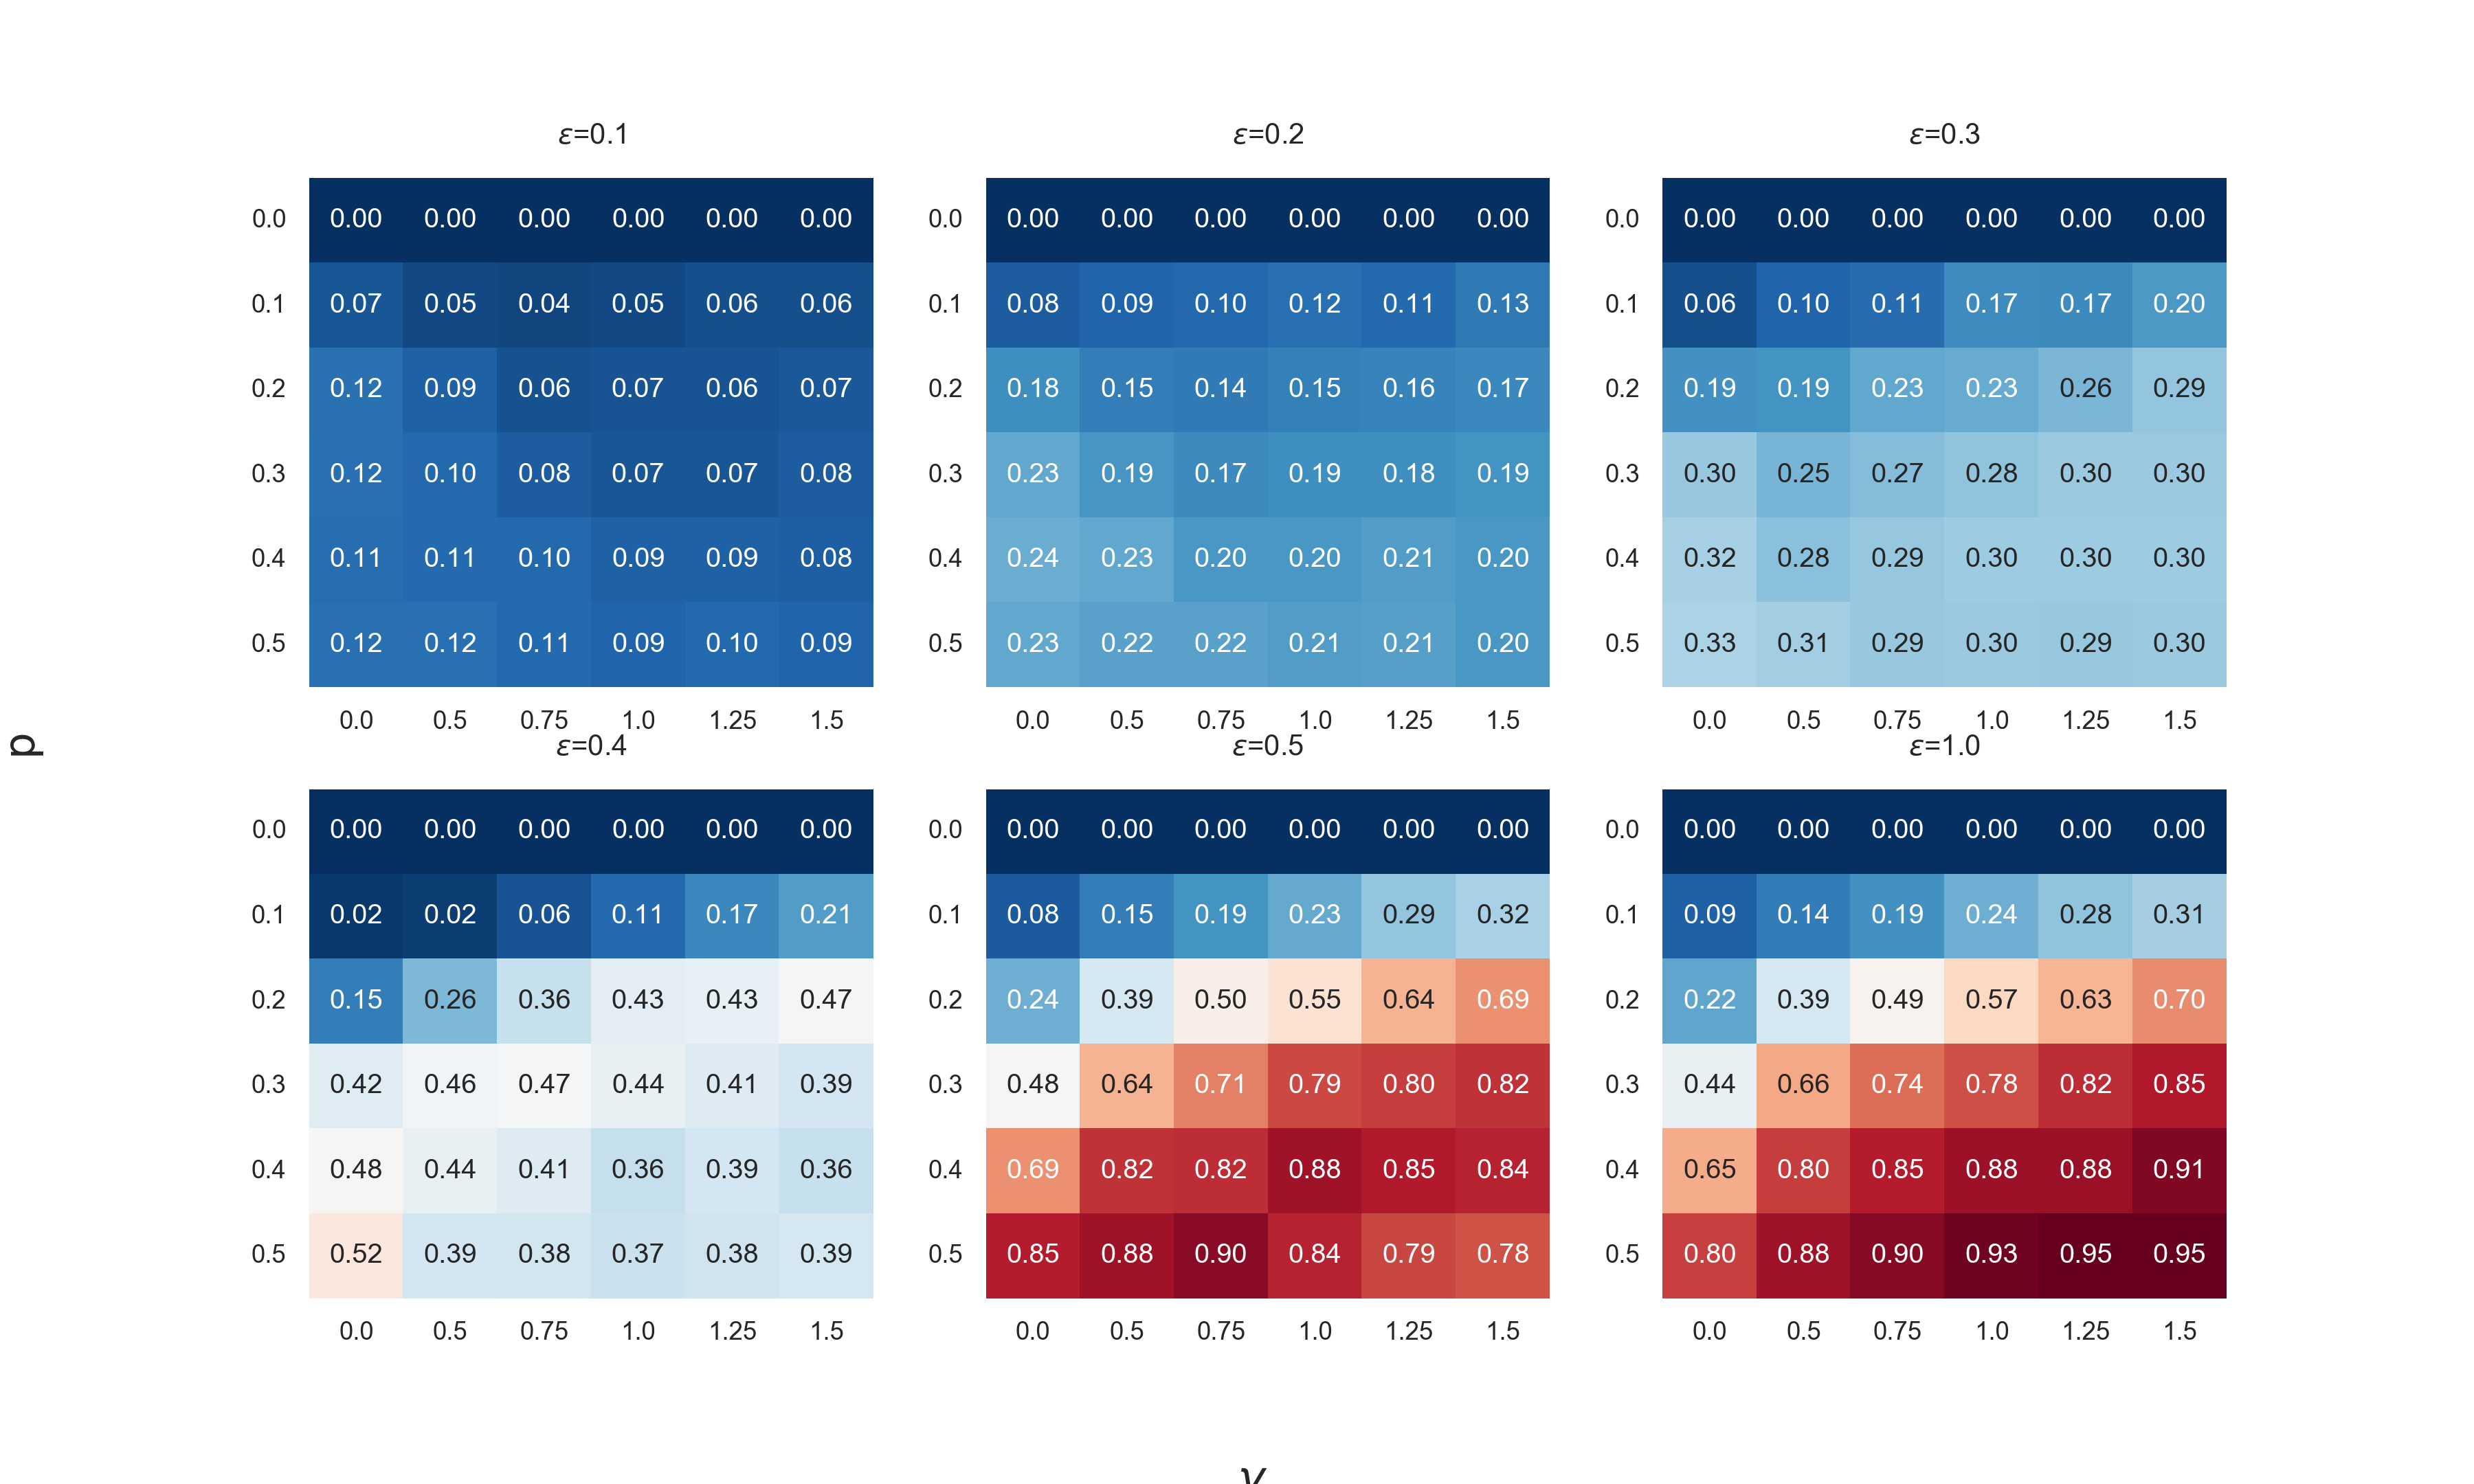
\includegraphics{figures/hm media mo0.0 perc_00 groupedby_eps.png}
    \caption{\textbf{Average percentage of nodes in $[0.0, 0.0001]$ in the case of one extreme media for different values of $\epsilon$ as a function of $\gamma$ and $p_m$.} As we can see for $\epsilon = 0.2$ the percentage of nodes in the \say{extremists} cluster is very similar across different combinations of $p_m$ and $\gamma$ always around $0.15-0.20$, except for $p=0.1$ where the values grows from $0.08 $ to $0.13$ as $\gamma$ increased. For $\epsilon =0.3$ the percentage grows with $\gamma$ for $p \leq 0.2$, while it stays around $0.25/0.30$ for $\p_m > 0.2$. For $\epsilon = 0.4$ it grows with $\gamma$ for $p_m \leq 0.2$ and it decreases with $\gamma$ for $p_m > 0.2$. For $\epsilon = 0.5$ it grows with $\gamma$ for $p_m \leq 0.4$ while it grows for $\gamma \leq 0.75$ and then decreases for $p_m=0.5$.}
    \label{fig:00avgextremeperc}
\end{figure}

\begin{figure}
    \centering
    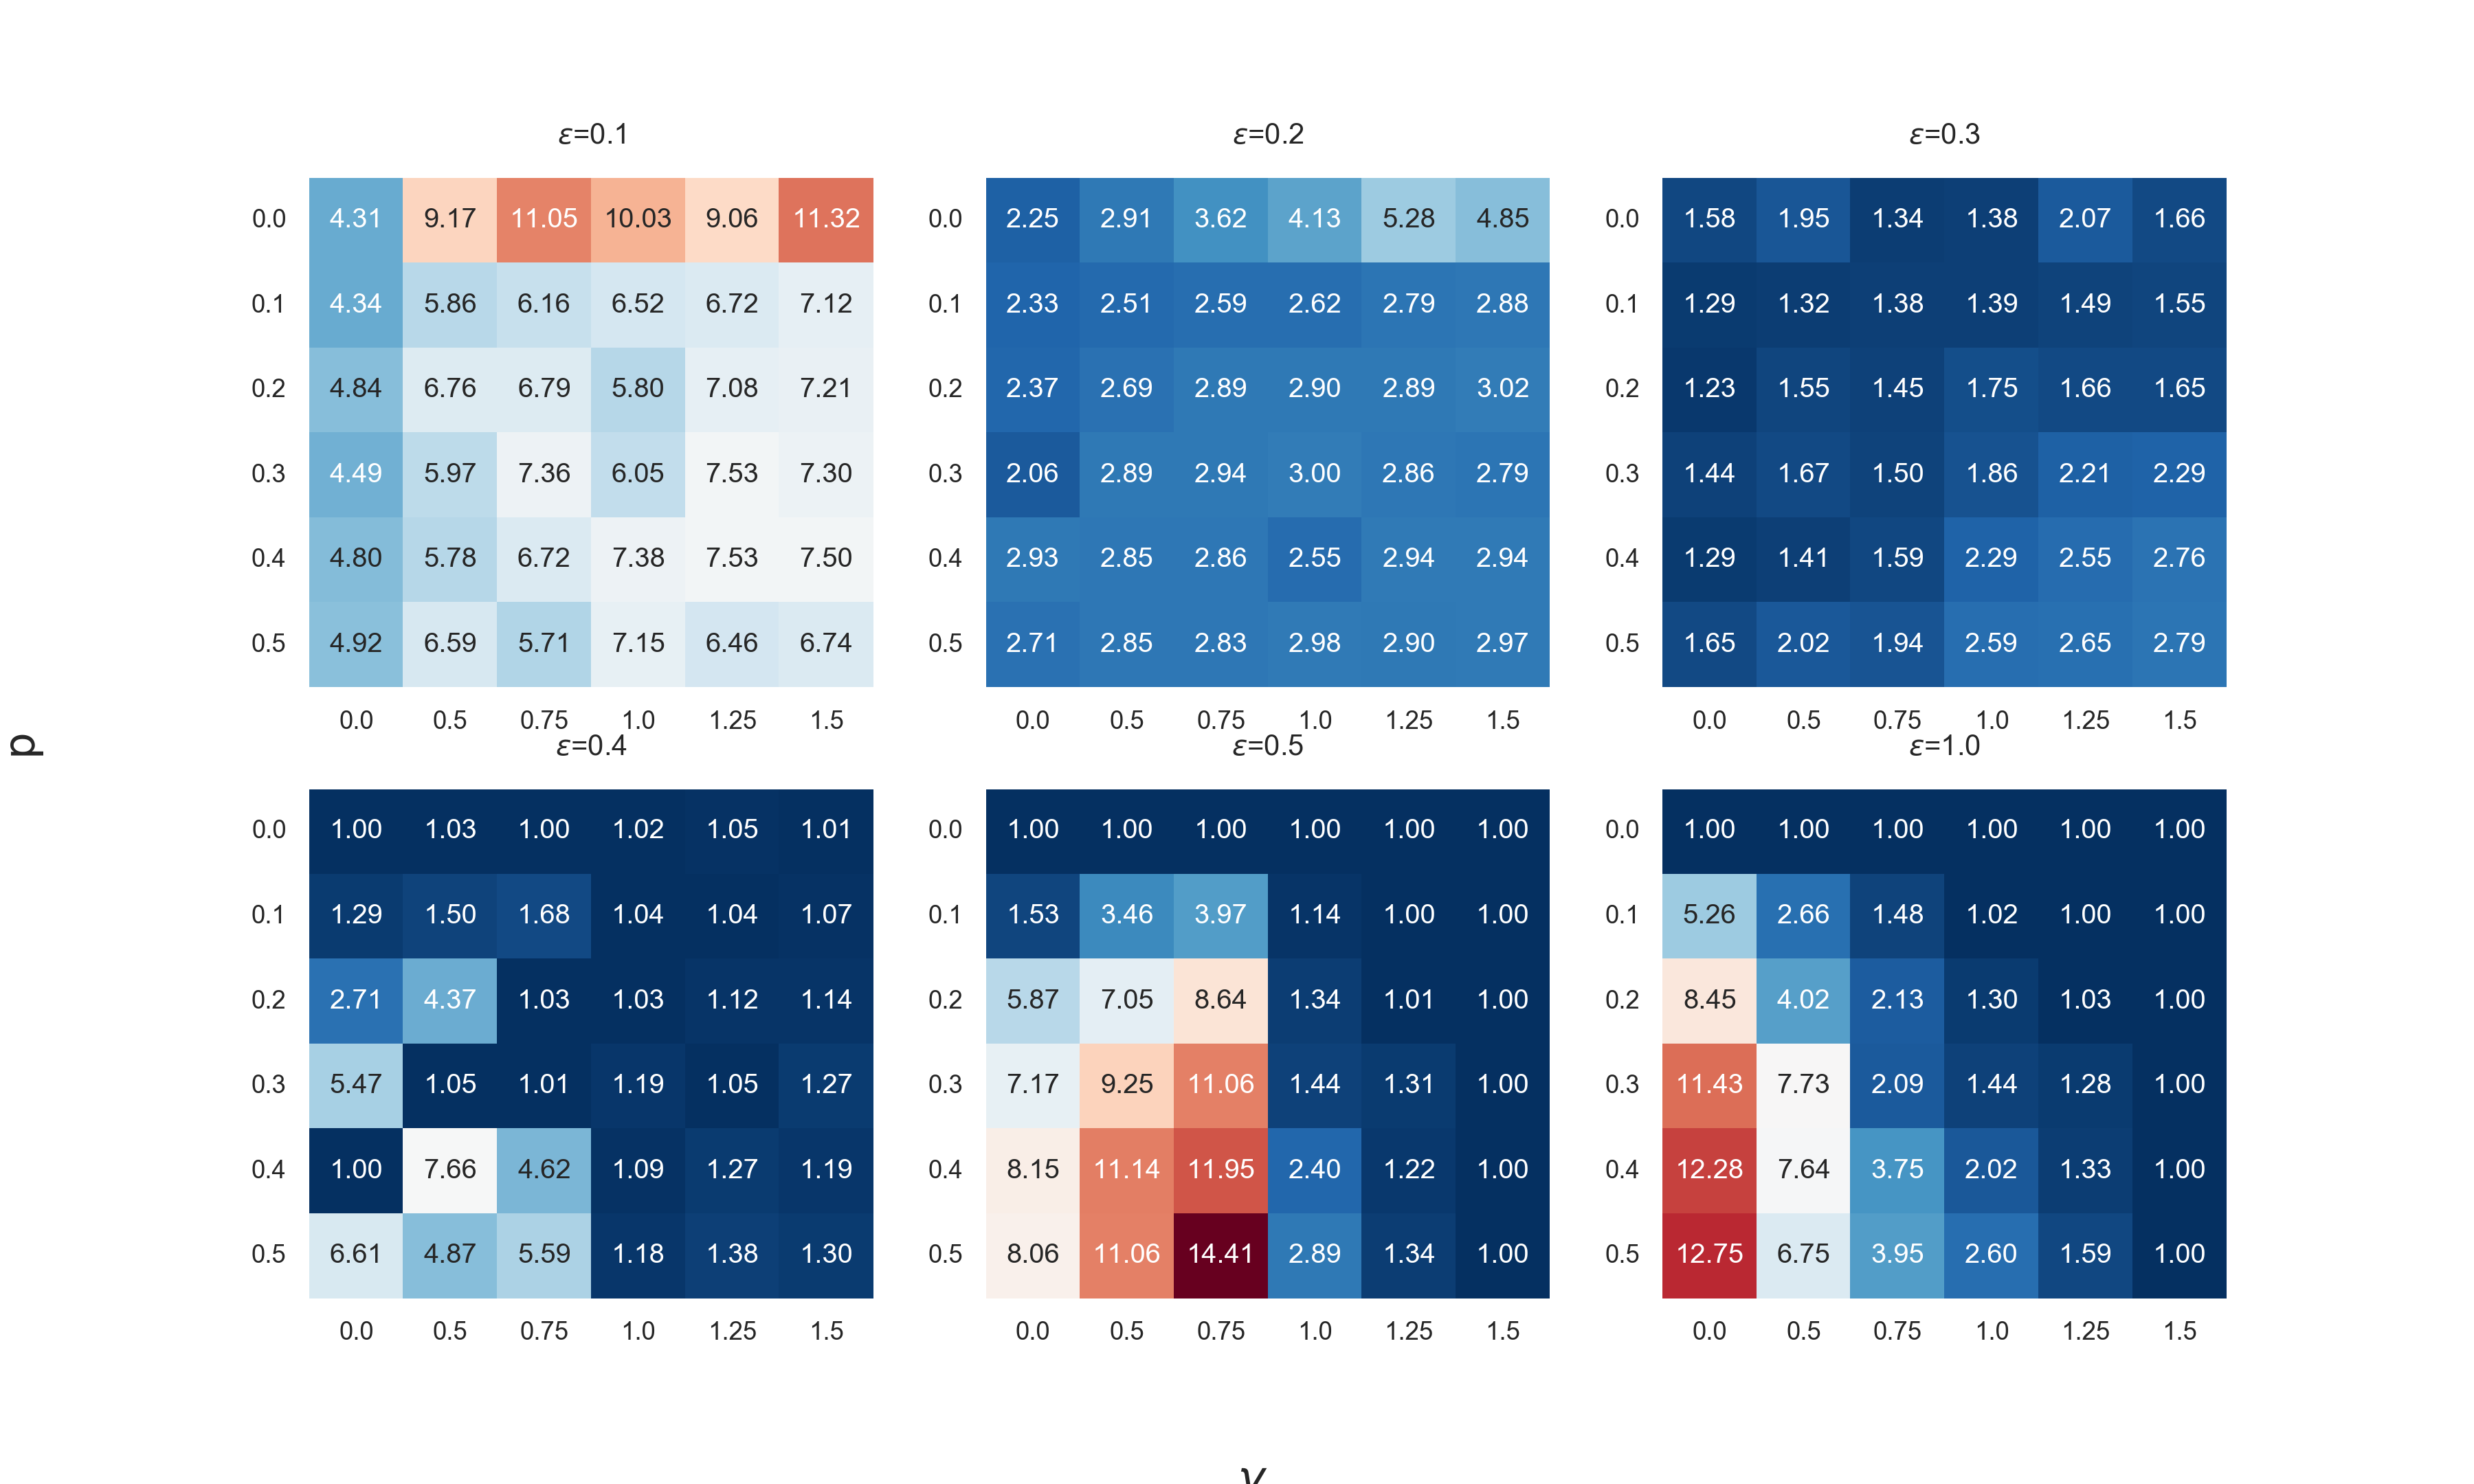
\includegraphics{figures/hm media mo0.05;0.5;0.95 0.01MS_avg_ncluster groupedby_eps.png}
    \caption{\textbf{Average number of clusters with two extreme media and a centrist one.} In this figure we can see the average number of clusters when there are three media, two of them hold extreme opinions on opposite sides of the opinion spectrum, and one of them holds the middle opinion. In the case of $\epsilon=0.2$ we can see that without any media the number of clusters grows with $\gamma$: in the DW model $\gamma=0$) the population is in a situation of polarisation, while already with $\gamma=0.5$ there are three clusters and the number grows with $\gamma$ up to $5$ clusters. When the media are added to the model we can see how the number of clusters slightly grows with $p_m$ when the bias is low, while for higher biases we always have around $3$ clusters, which means that fragmentation is reduced by combining media and bias with respect to the model with no media, probably due to the fact that media tend to \say{attract} a portion of the population and in the end clusters form around the media opinions. For $\epsilon=0.3$ without media we go from consensus to polarisation as $\gamma$ grows. However, as $p_m$ also grows we go from consensus to three clusters or from polarisation to three clusters. In the case of $\epsilon=0.4$ and $\epsilon=0.5$ the behaviour is very different, probably due to the fact that this is more or less the distance between one media and the other. In this case we have a higher fragmentation for high values of $p_m$ but low values of $\gamma$, which is higher and higher as $\epsilon$ grows. This is probably due to the fact that even if nodes are attracted to one media in one iteration, they can encounter another media in the next iteration and move in the opinion spectrum, without ever converging to an equilibrium. As the bias grows, however, nodes tend to interact only with the ones already close to them so this behaviour is mitigated and the system can actually reach a consensus, probably due to the fact that once a node is attracted by the middle media, it stays in that cluster due to algorithmic bias and sooner or later all the nodes will encounter that media due to a high $p_m$.}
    \label{fig:3mediaavgnclusterbyeps}
\end{figure}

\begin{figure}
    \centering
    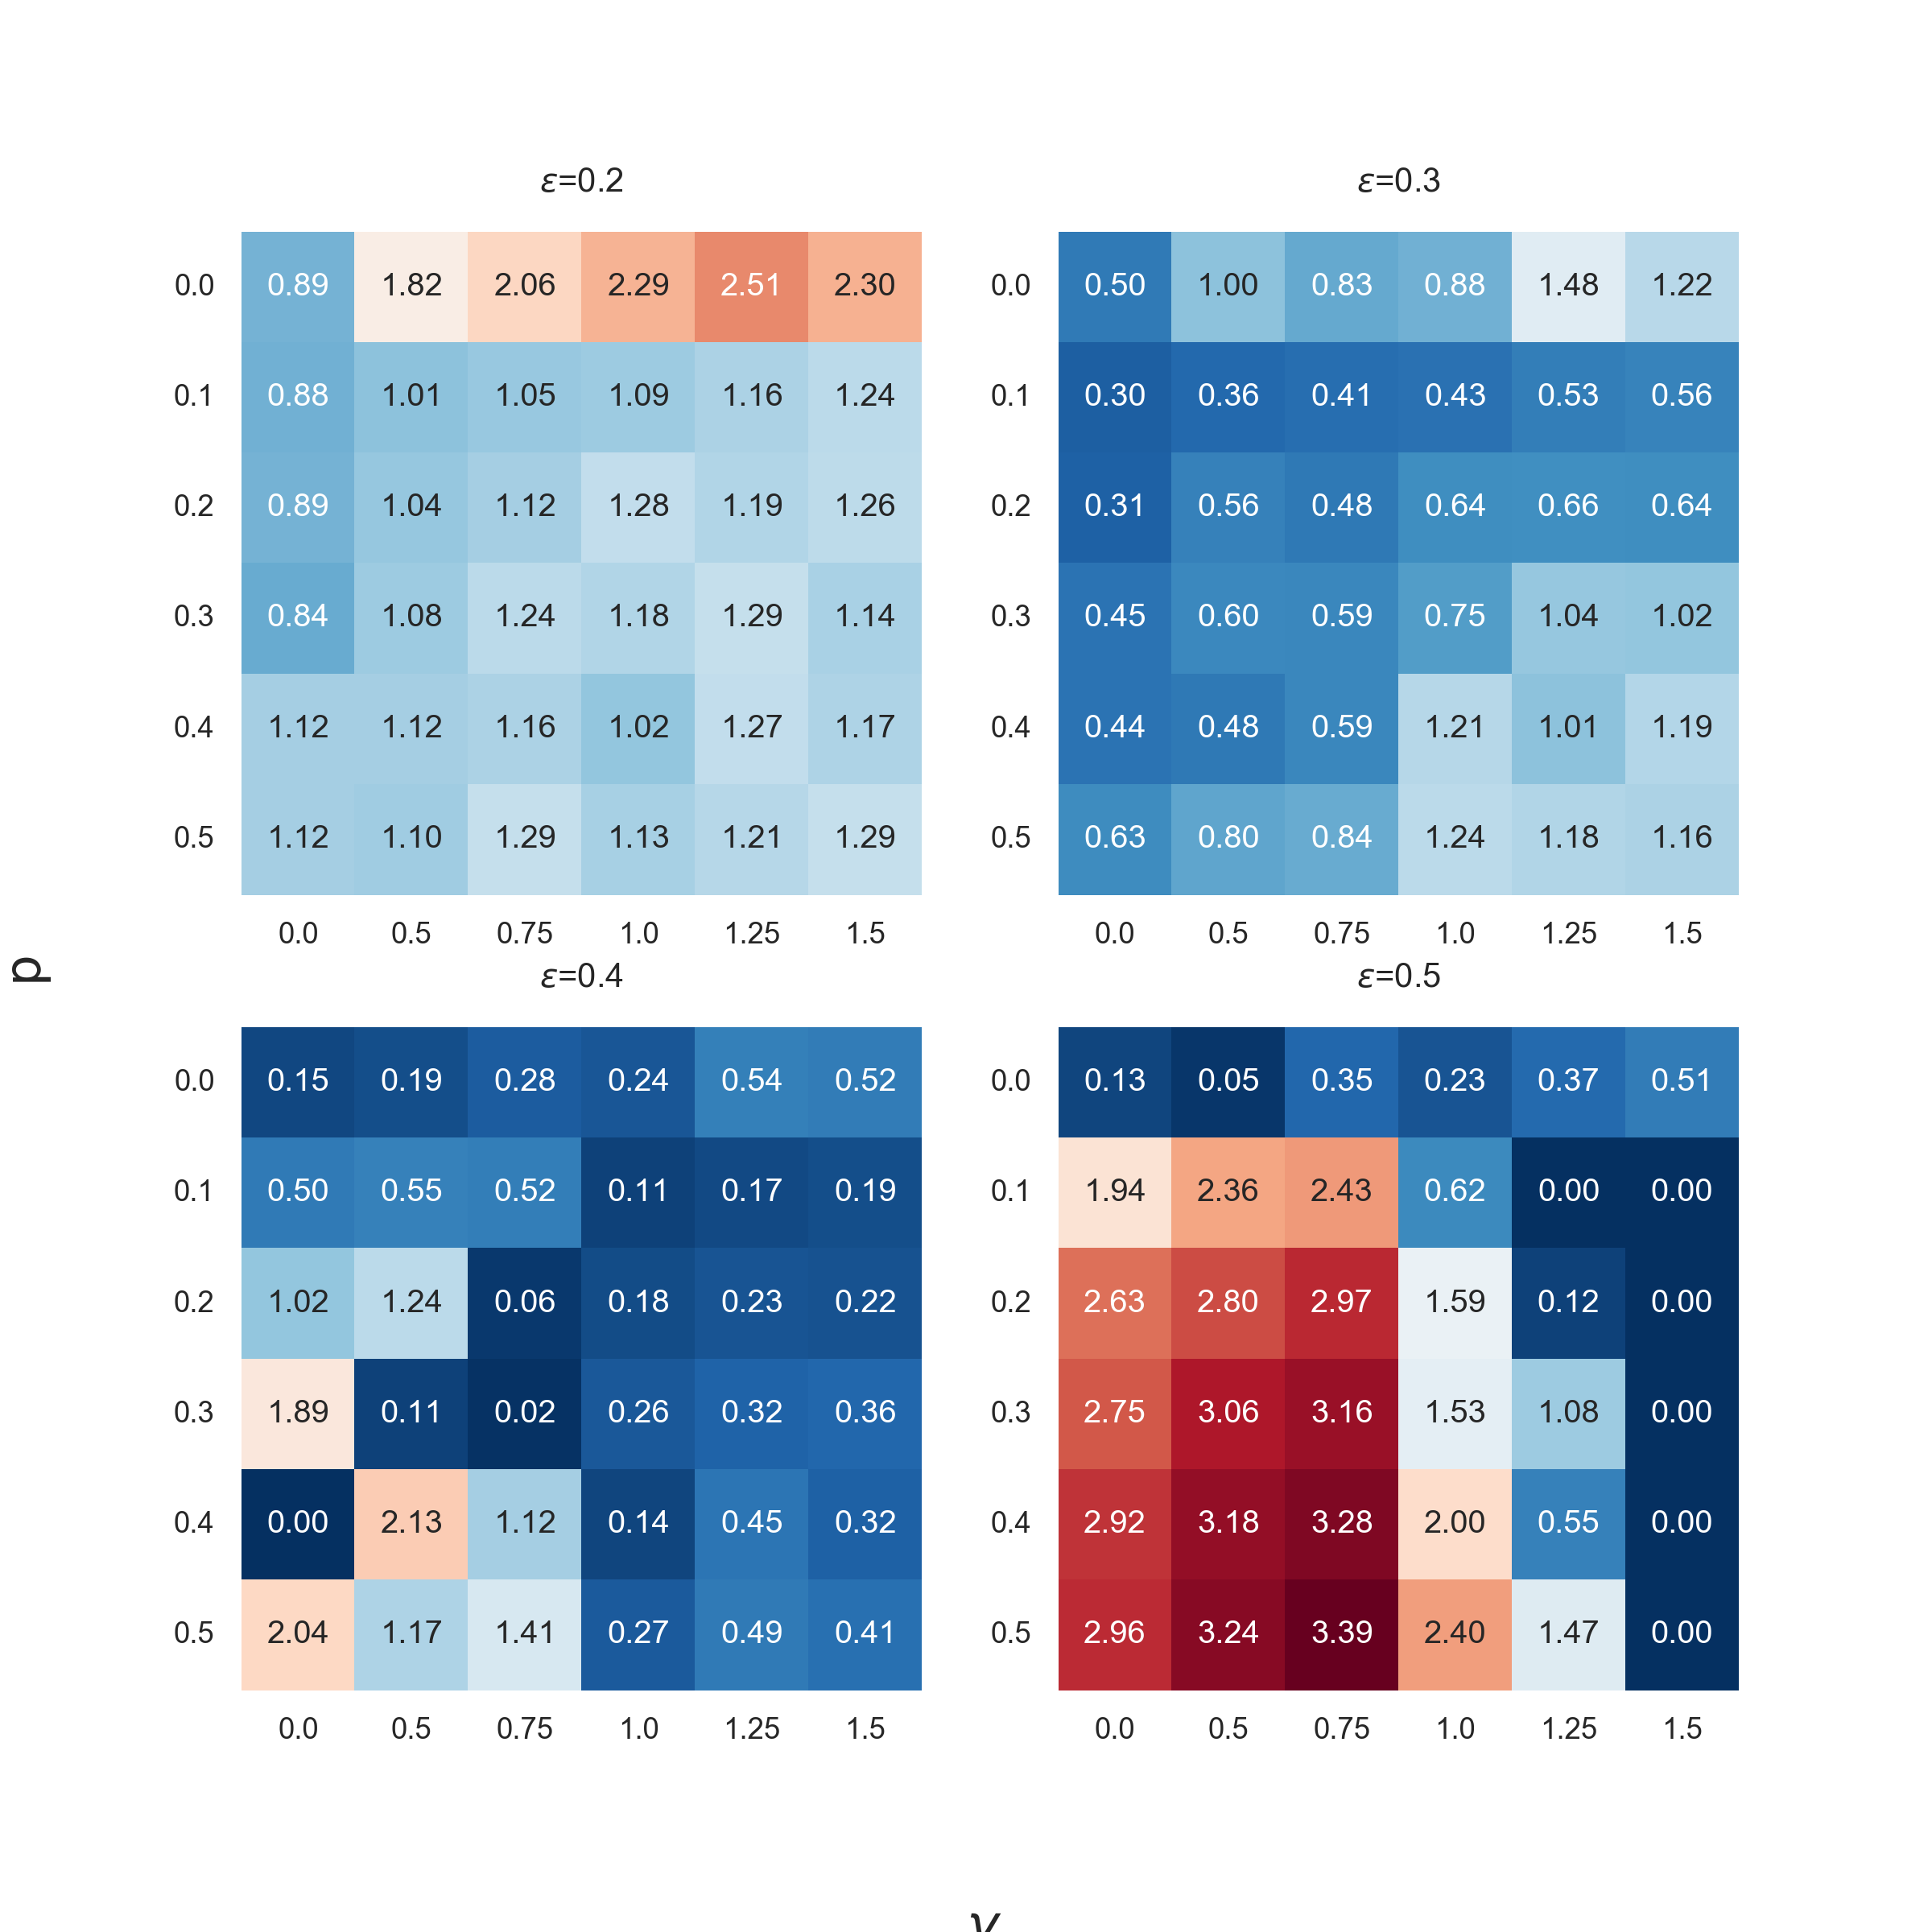
\includegraphics{figures/hm media mo0.05;0.5;0.95 10B_avg_entr groupedby_eps.png}
    \caption{\textbf{Average entropy.} Also in this case entropy follows more or less the same behaviour seen in the average number of clusters.}
    \label{fig:3mediaavgentrbyeps}
\end{figure}

\begin{figure}
    \centering
    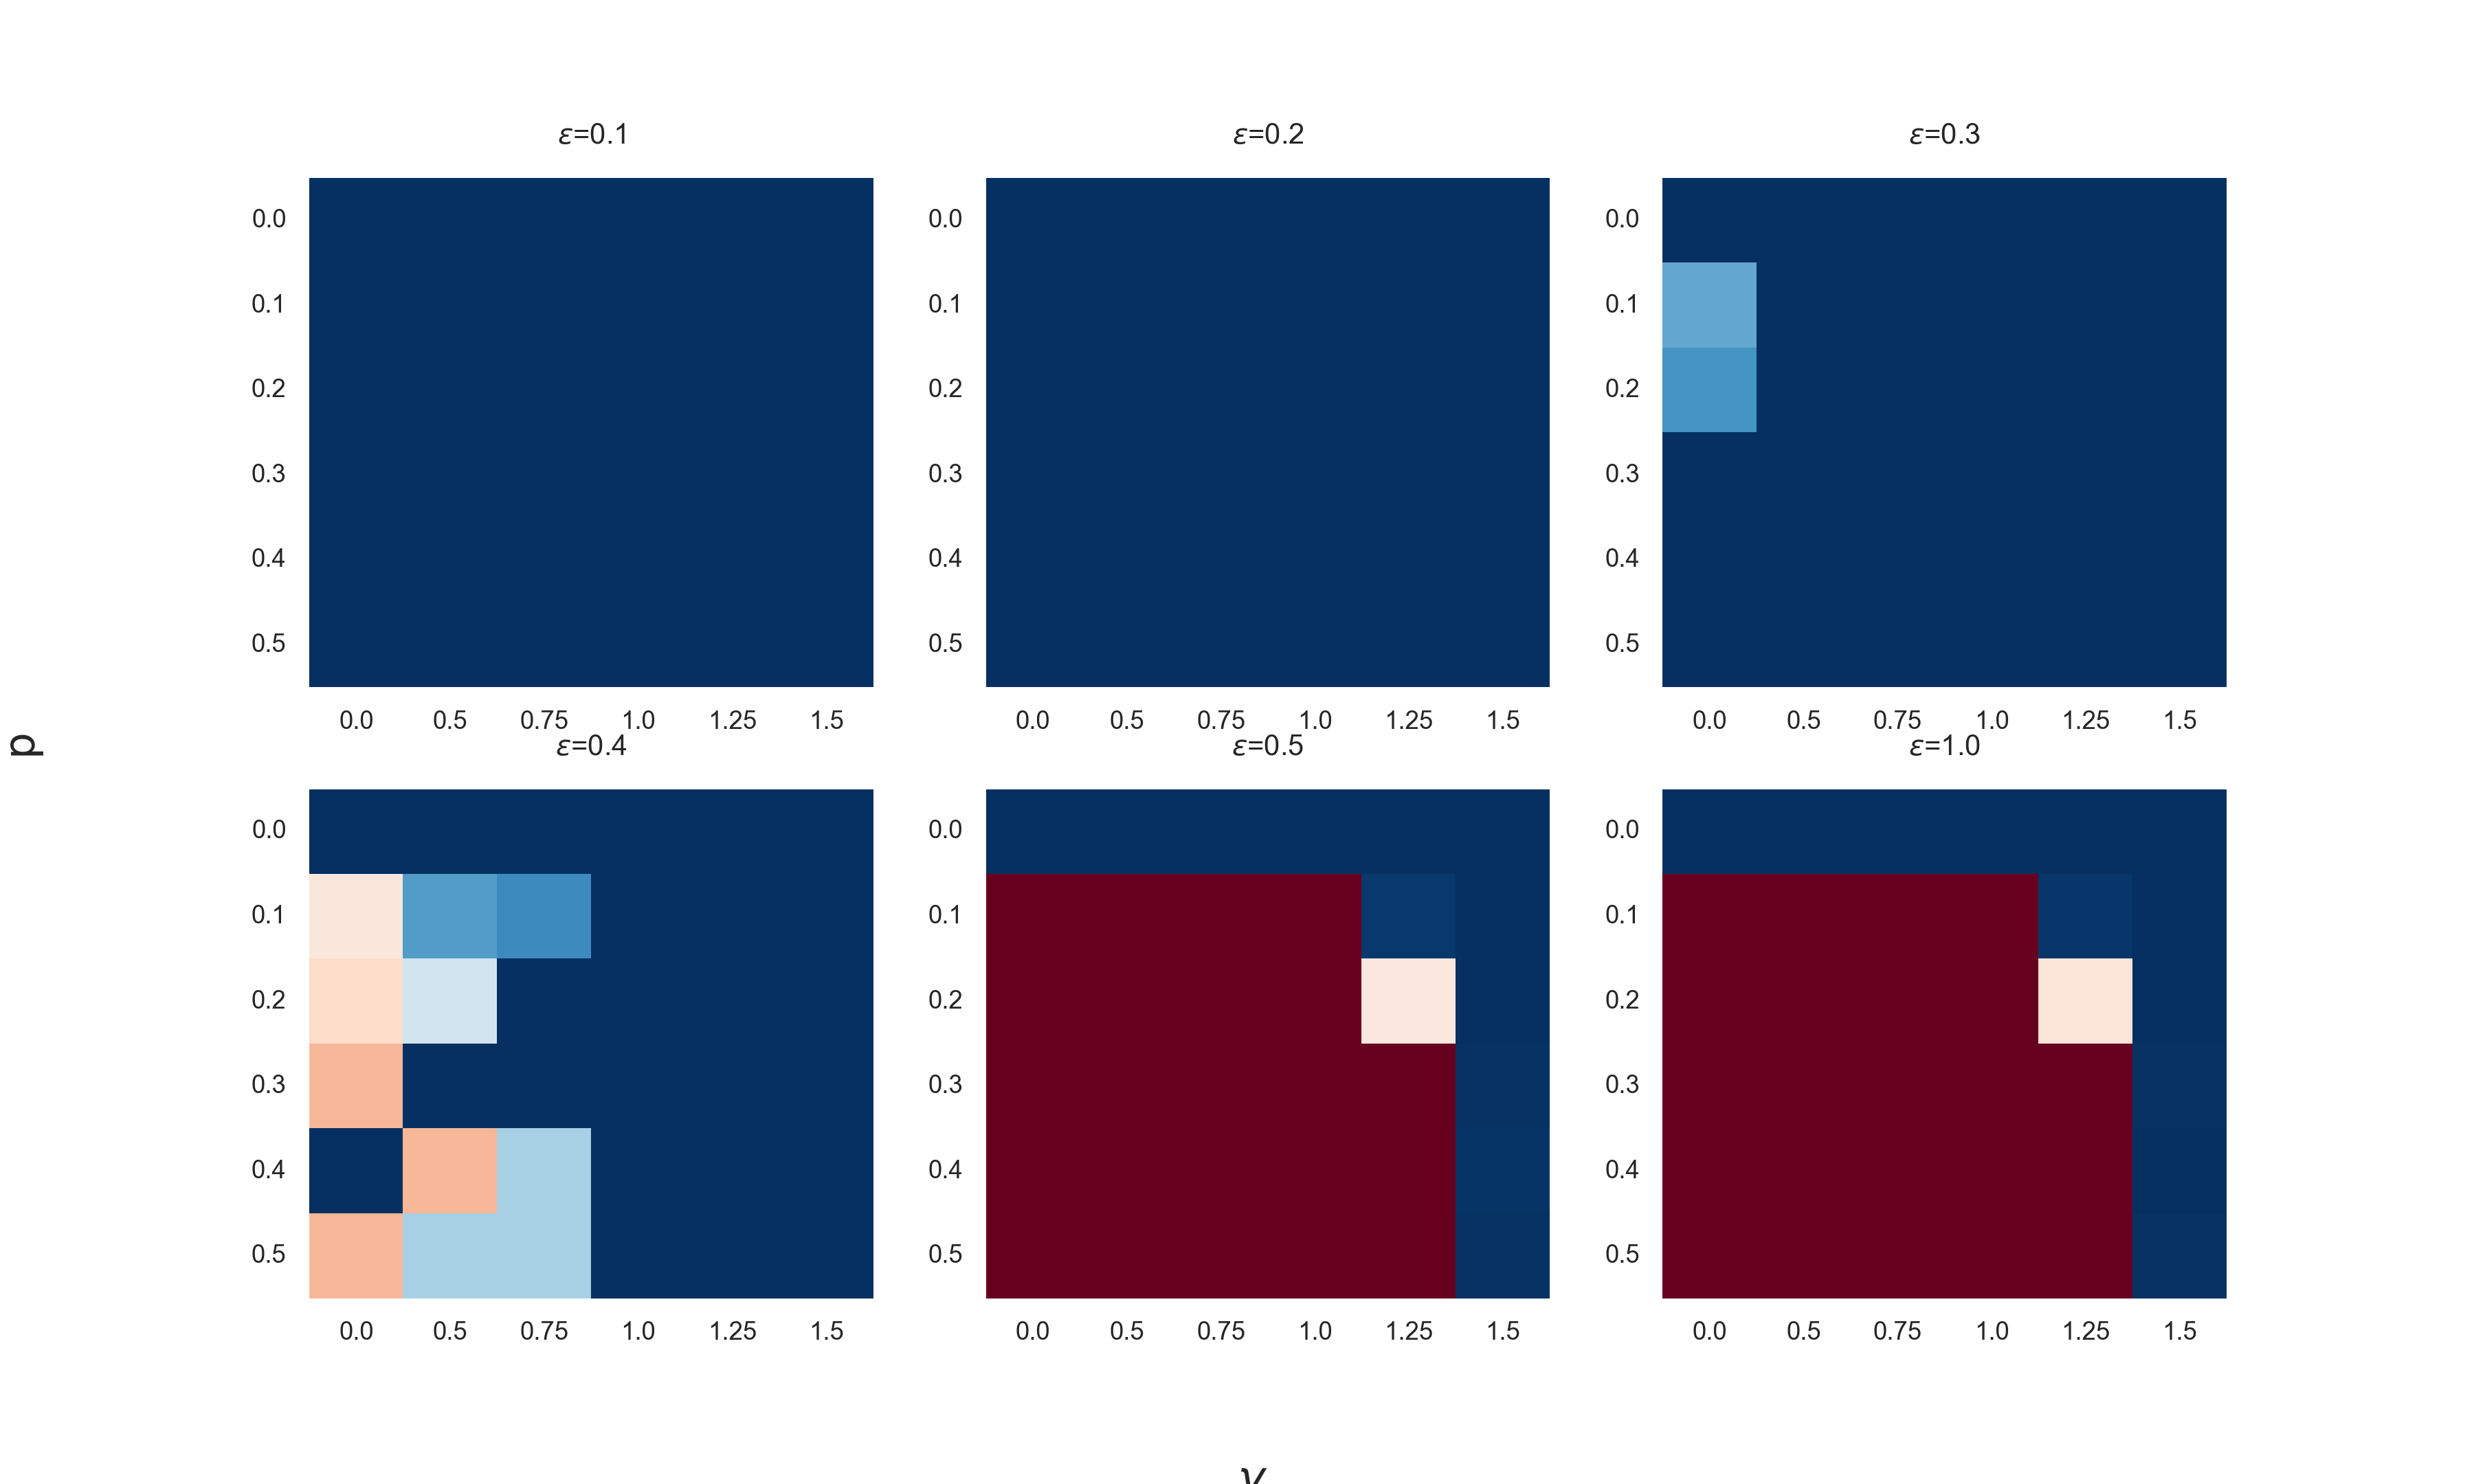
\includegraphics{figures/hm media mo0.05;0.5;0.95 avg_niter groupedby_eps.png}
    \caption{\textbf{Average number of iterations at convergence in the case of two extremist media and one moderate media.} As we can see while $\epsilon \leq 0.3$ convergence is pretty fast and moreover it seems to become faster as $\gamma$ grows, probably due to the fact that the clustering of agents around media opinions becomes faster when the interactions are biased. However we can see that in the cases where the nodes can be influenced by more than one media due to a higher confidence bound the system takes a very long time to reach equilibrium and, as the confidence bound $\epsilon$ grows, equilibrium cannot be reached anymore, so the maximum number of iterations is always reached.}
    \label{fig:3mediaavgniterbyeps}
\end{figure}

\begin{figure}
    \centering
    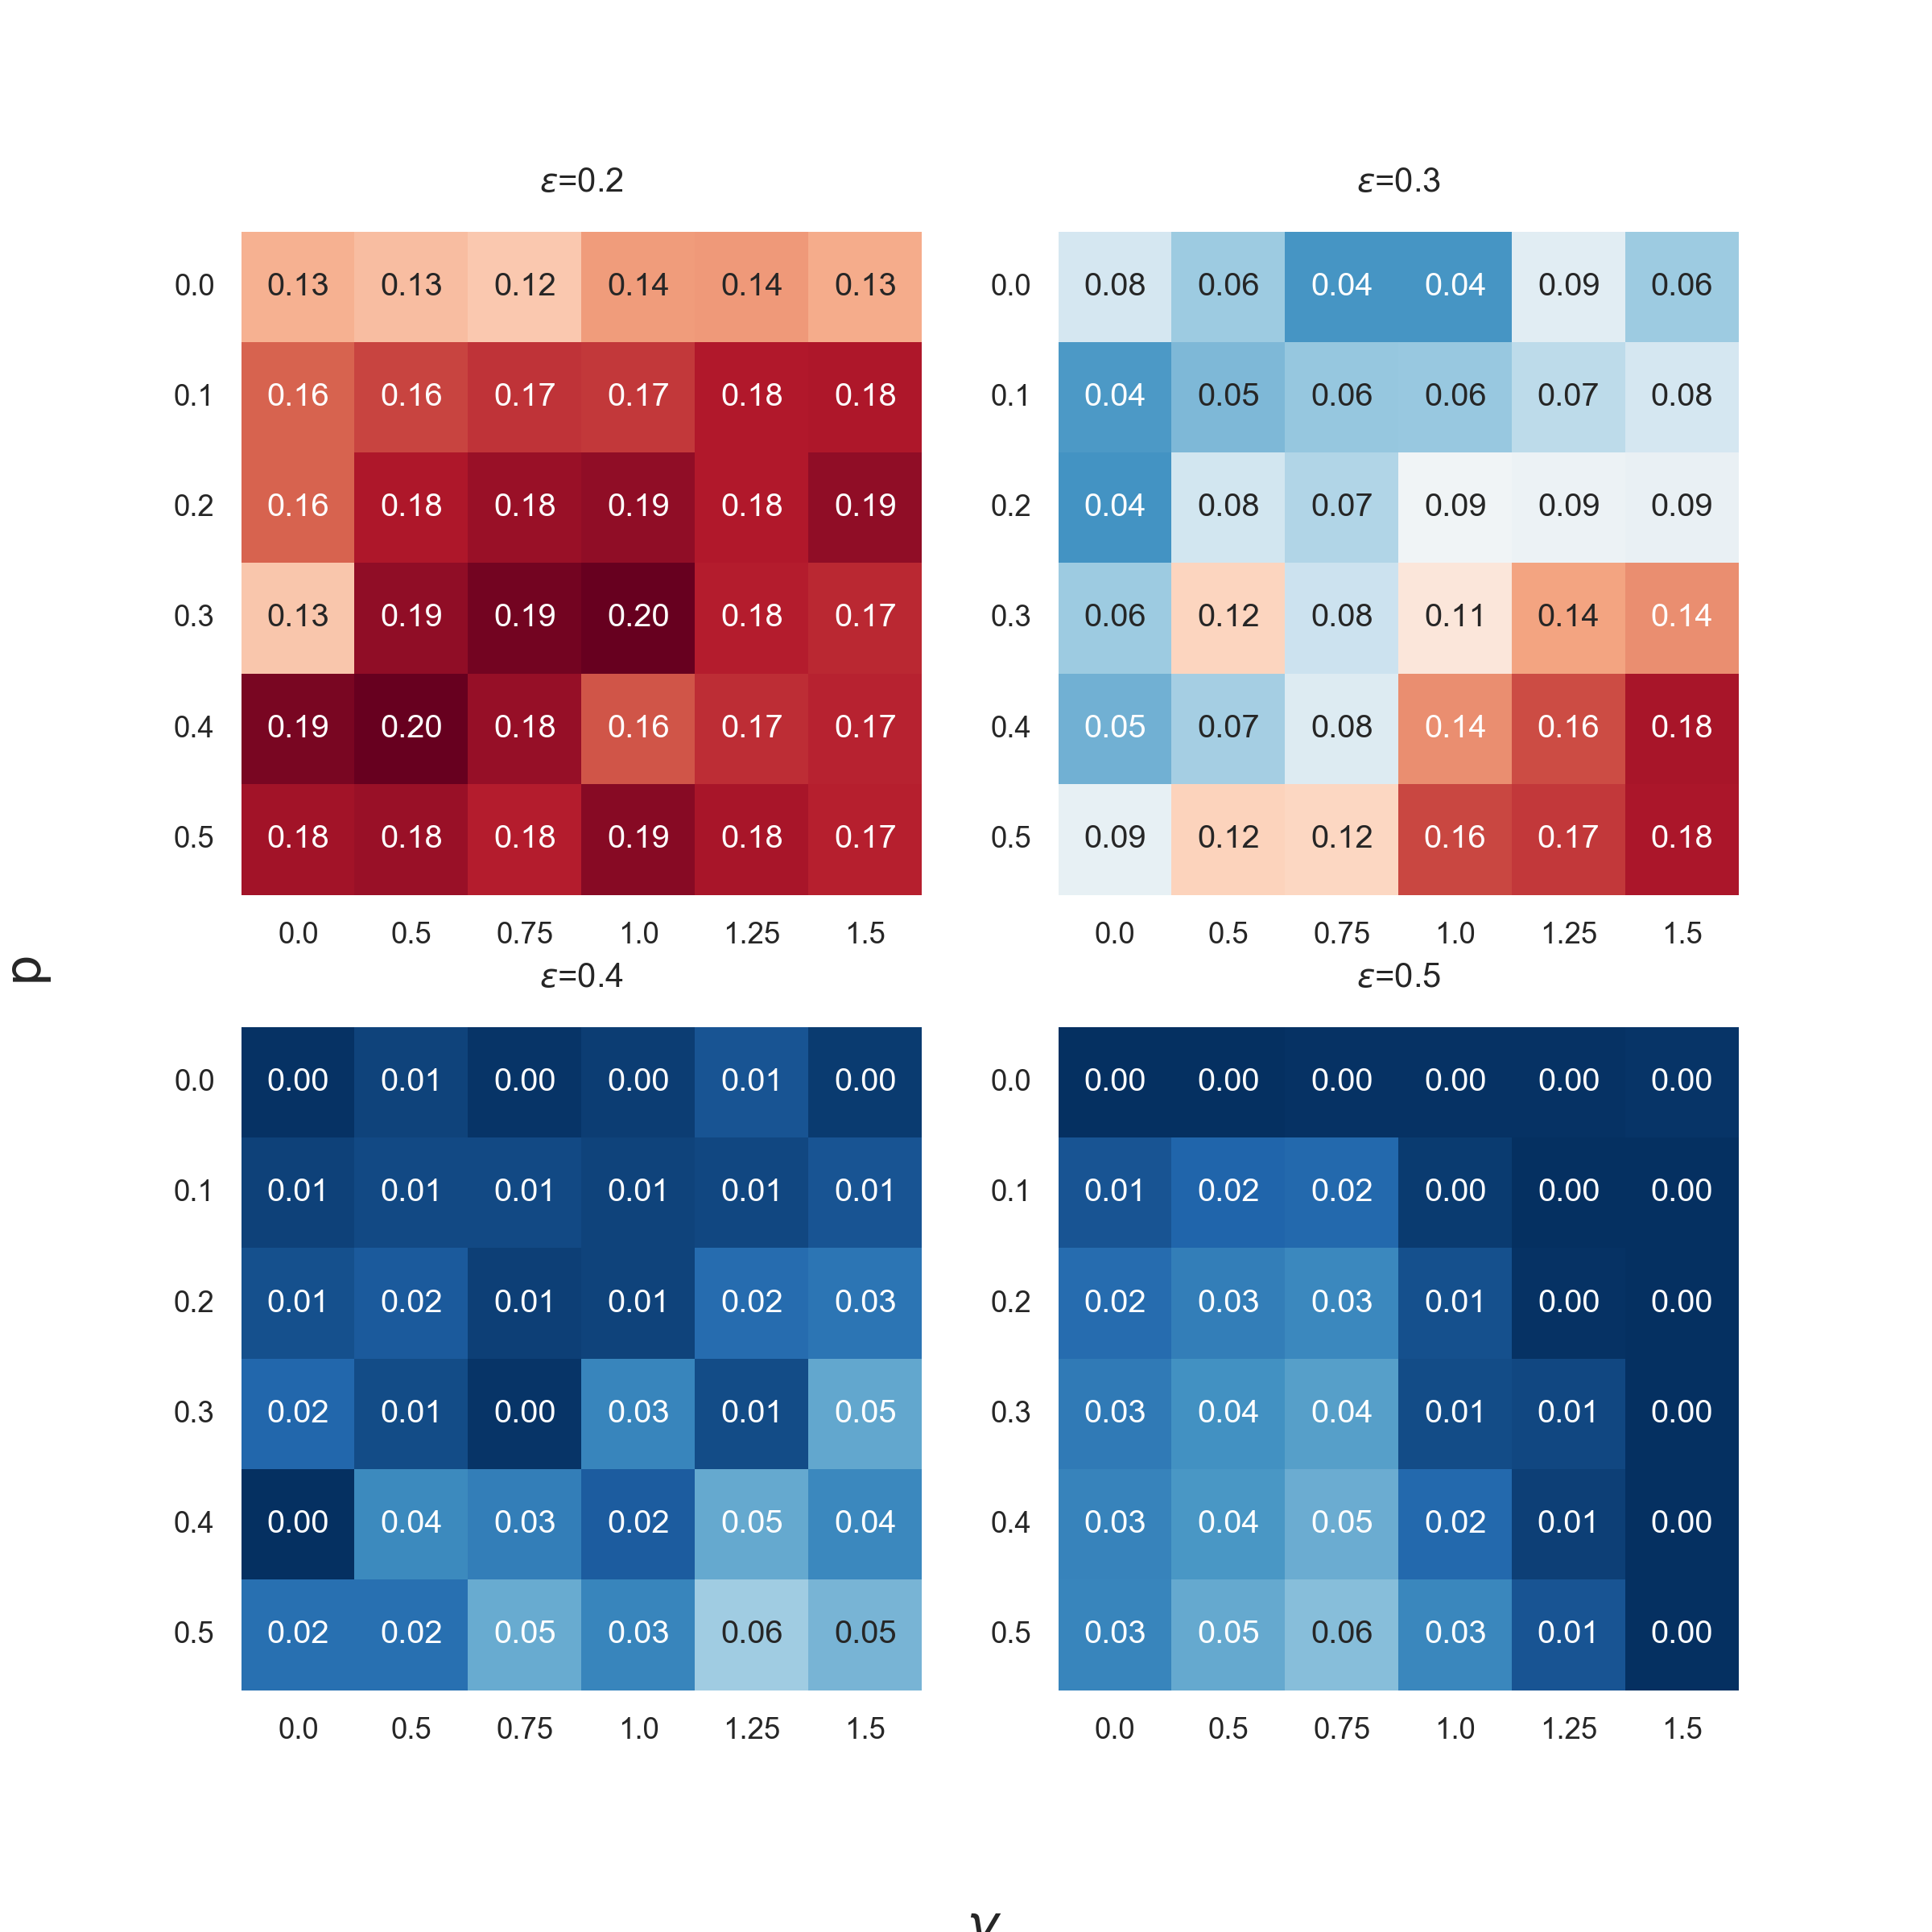
\includegraphics{figures/hm media mo0.05;0.5;0.95 avg_pwdist groupedby_eps.png}
    \caption{\textbf{Average pairwise distance in the case of two extremist media and one moderate media.} In this figure we can see the average pairwise distance which shows that when the average number of clusters or entropy are very high (in the case of $\epsilon \geq 0.4$ and $\gamma \leq 0.74 \text{or} 1.0$) the average pairwise distance is still close to 0, while in the case of polarisation/fragmentation in the baseline model we had an average pairwise distance greater than $0.10/0.15$. This shows how actually agents do not form any cluster but are evenly distributed within certain opinion values in the spectrum creating what could be seen as a single cluster, with a low average pairwise distance (so we don't have polarisation) but a high entropy. In these cases the three media do not attract agents in the sense that they end up splitting the population in three compact clusters. Instead, they restrict the overall opinion range within which agents are distributed, which can be between two of the three media or between all three.}
    \label{fig:3mediaavgpwdistbyeps}
\end{figure}

\begin{figure}
    \centering
    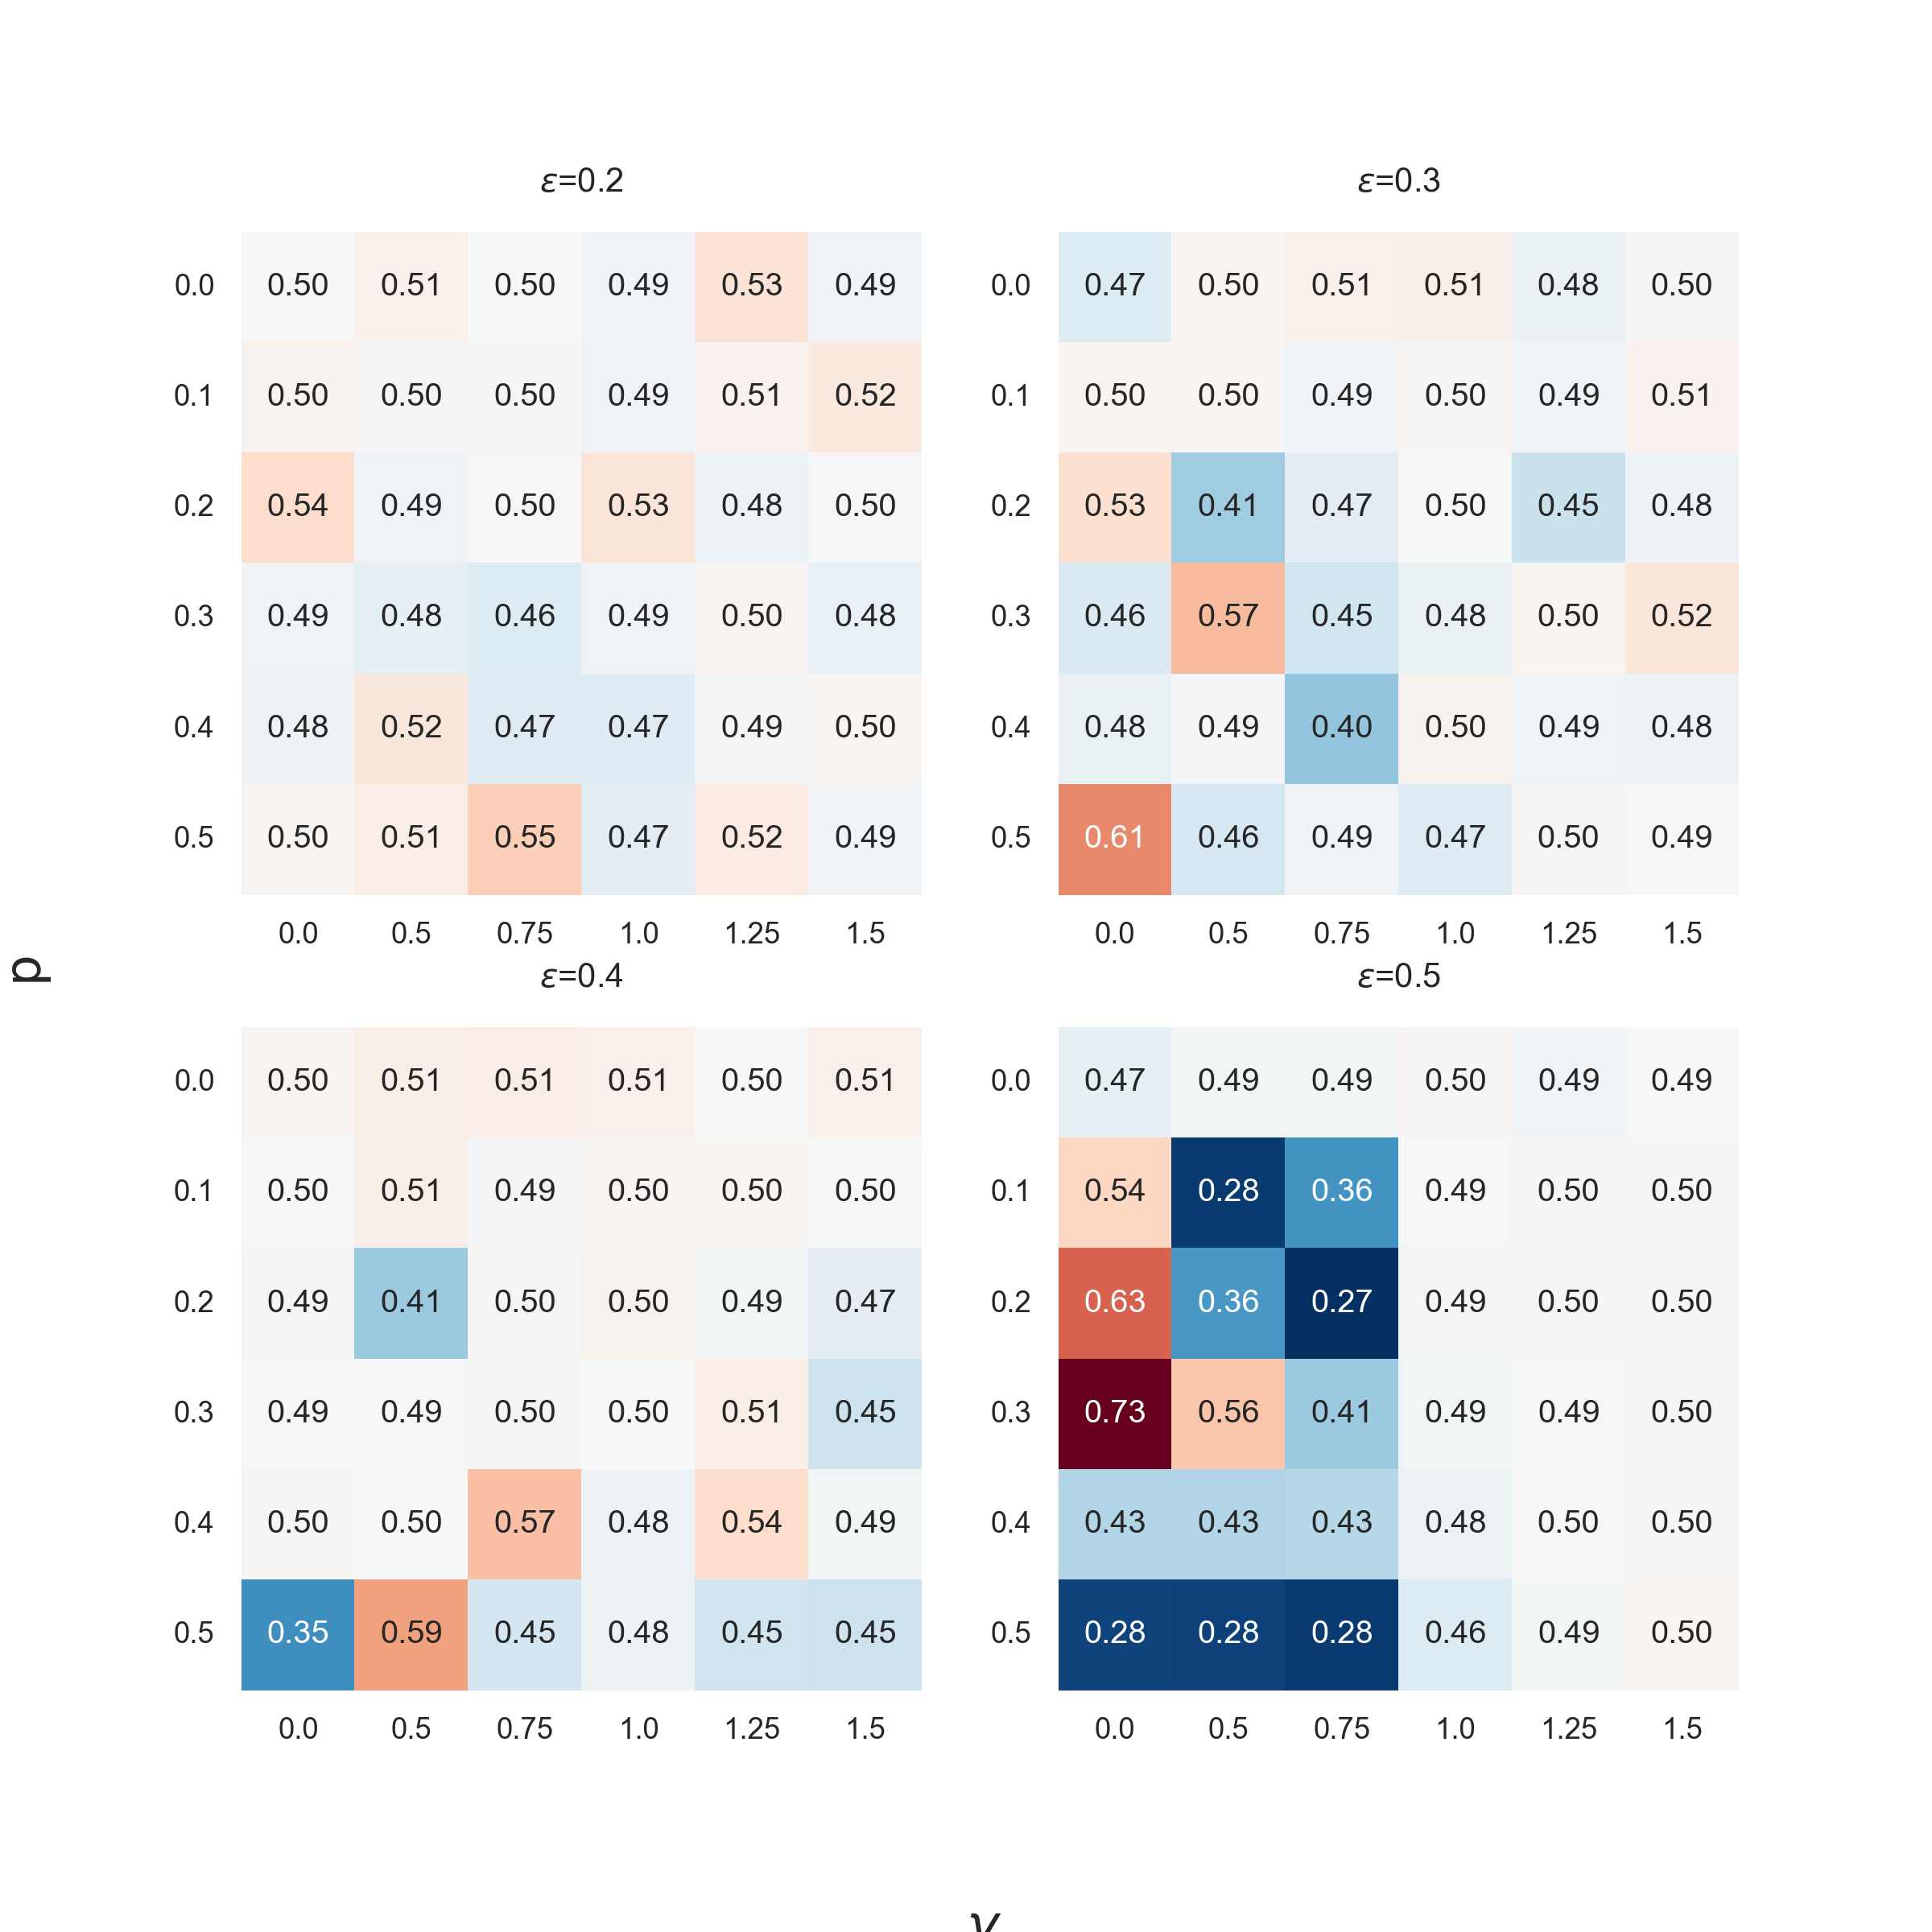
\includegraphics{figures/hm media mo0.05;0.5;0.95 avg_opinion groupedby_eps.png}
    \caption{\textbf{Average opinion.} As we can see from the figure for $\epsilon \leq 0.3$ the average opinion is always around the mean opinion, sometimes a little above and sometimes a little lower, but pretty much always around $0.5$. This also happens for $\epsilon=0.4$ actually even for the cases where entropy was higher, except the cases where $p=0.5$ and there is no bias. However, we can see in the case of $\epsilon=0.5$ that the mean opinion can be very higher than 0.5 or very lower, meaning that agents are grouped within two of the three media, shifting the mean opinion.} 
    \label{fig:3mediaavgopbyeps}
\end{figure}

\begin{figure}
    \centering
    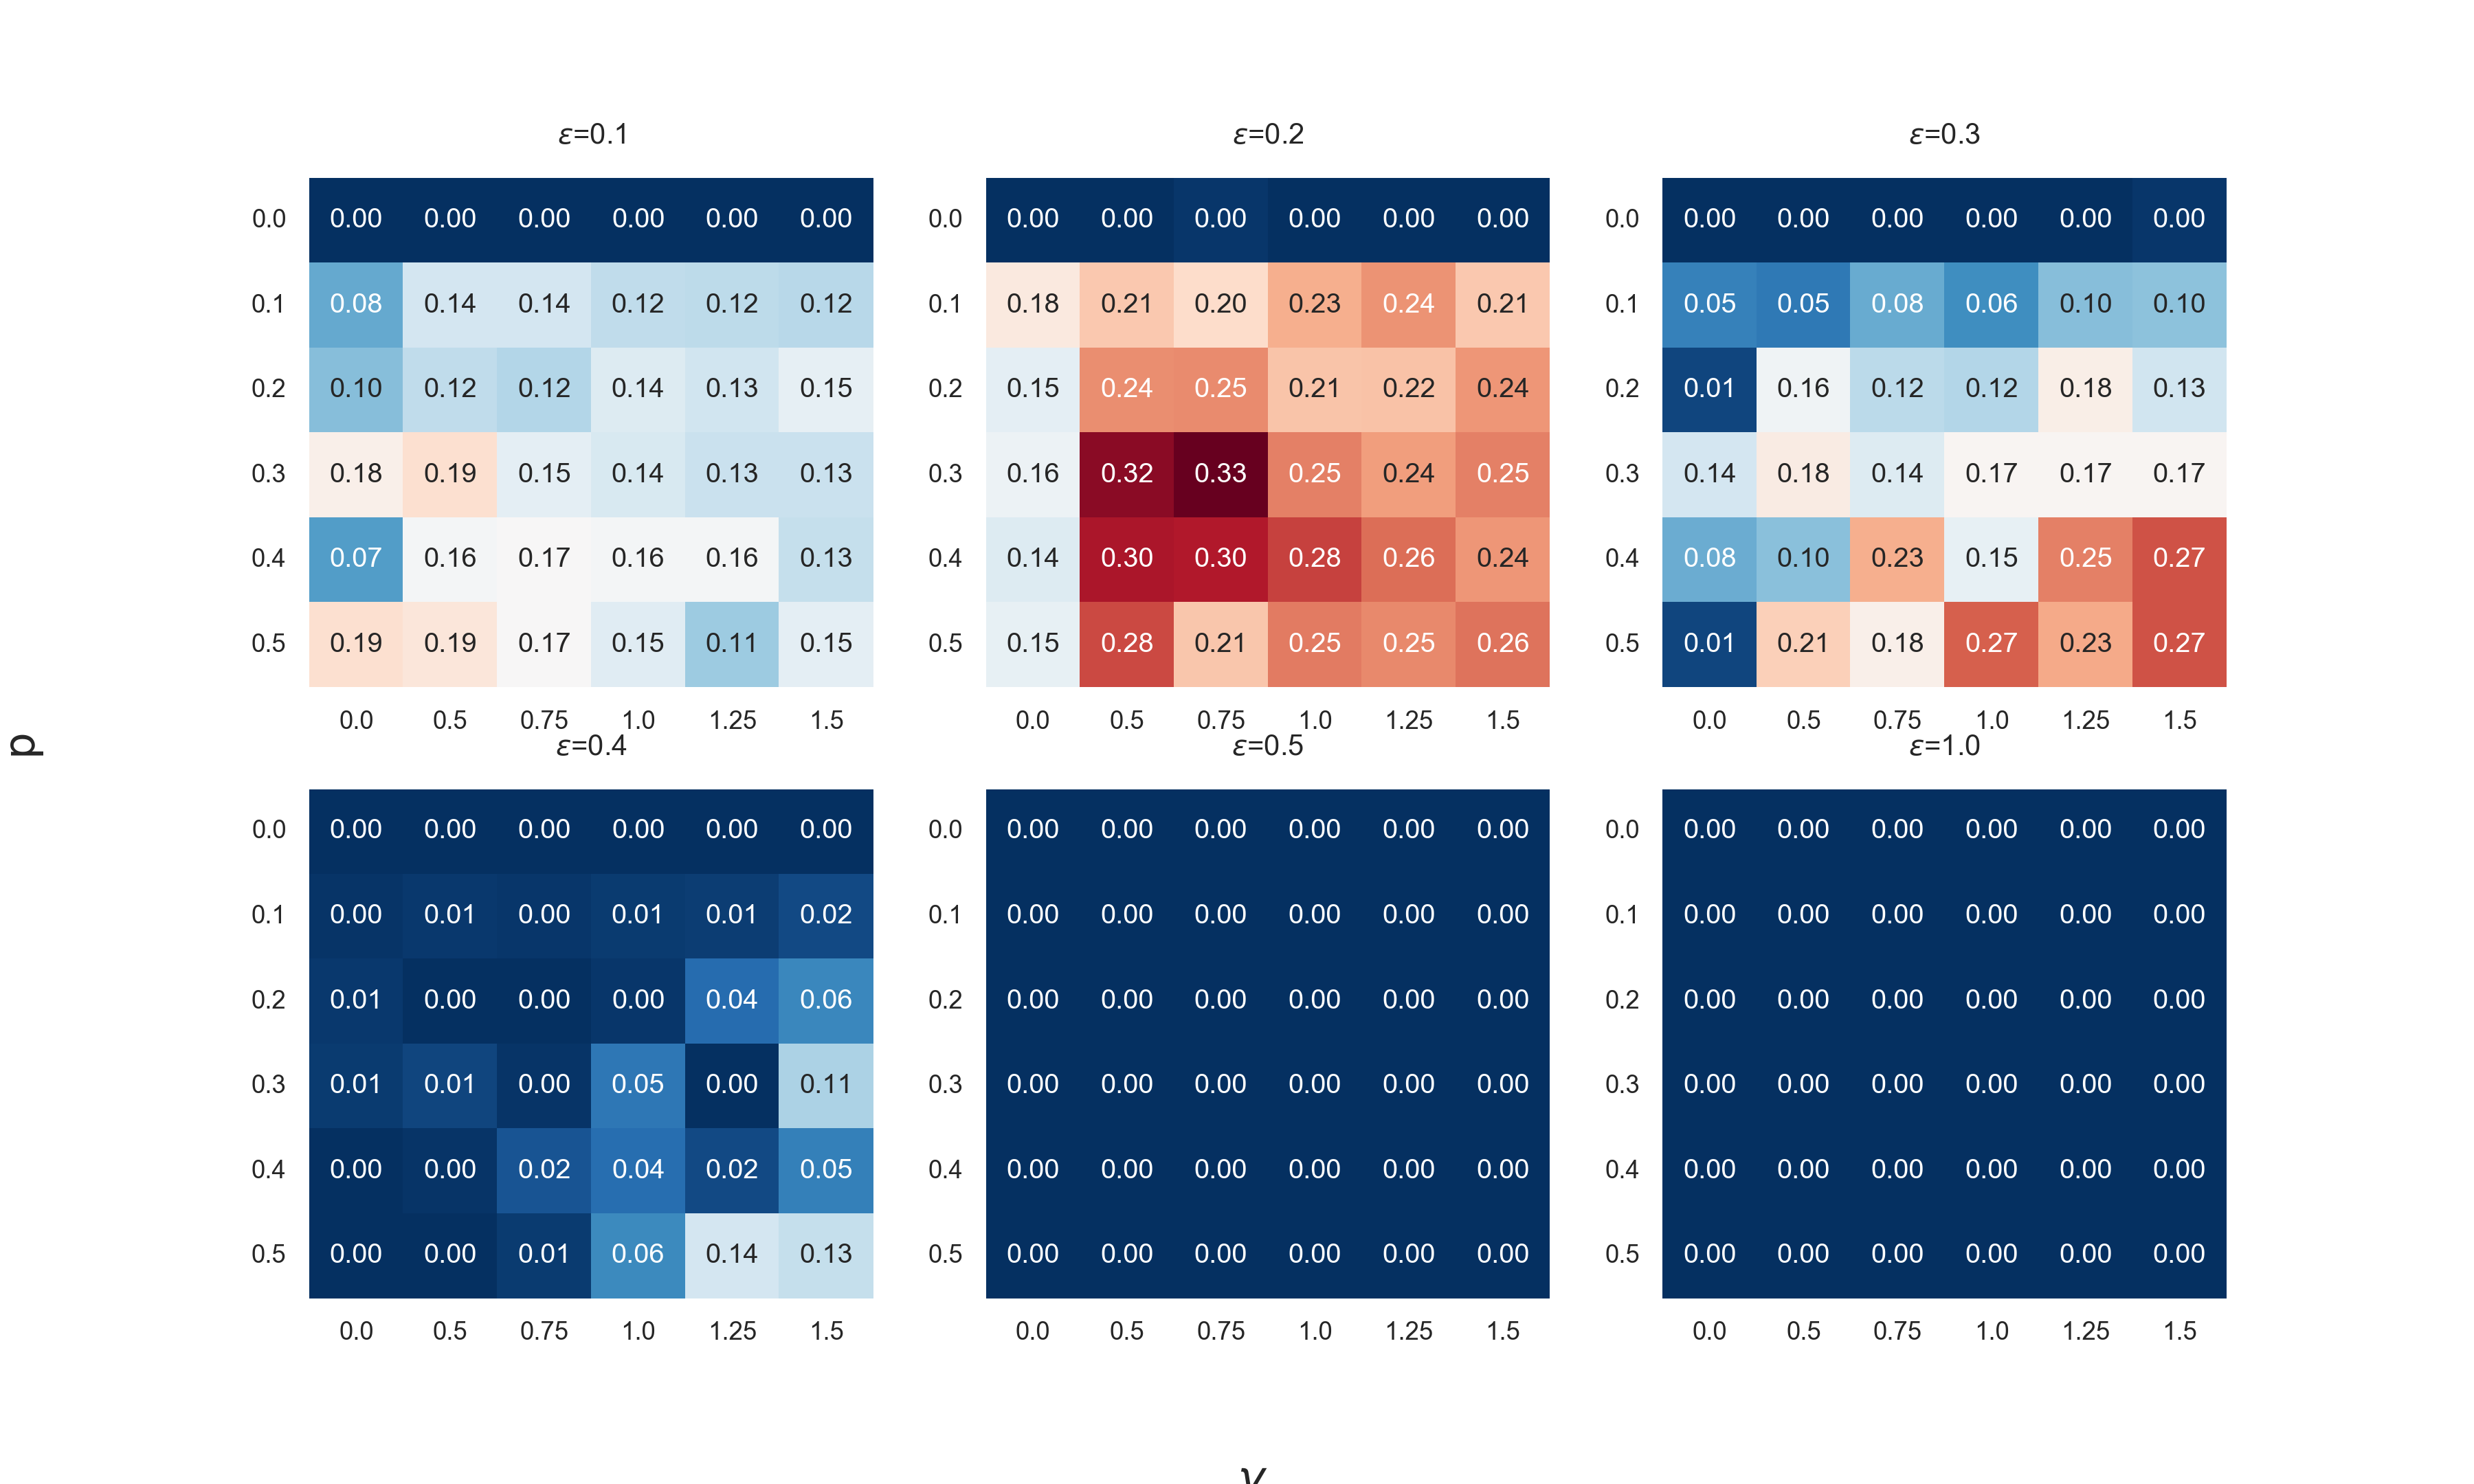
\includegraphics{figures/hm media mo0.05;0.5;0.95 perc_005 groupedby_eps.png}
    \caption{\textbf{Percentage of nodes around the lower extreme media.}}
    \label{fig:3mediaperc005byeps}
\end{figure}

\begin{figure}
    \centering
    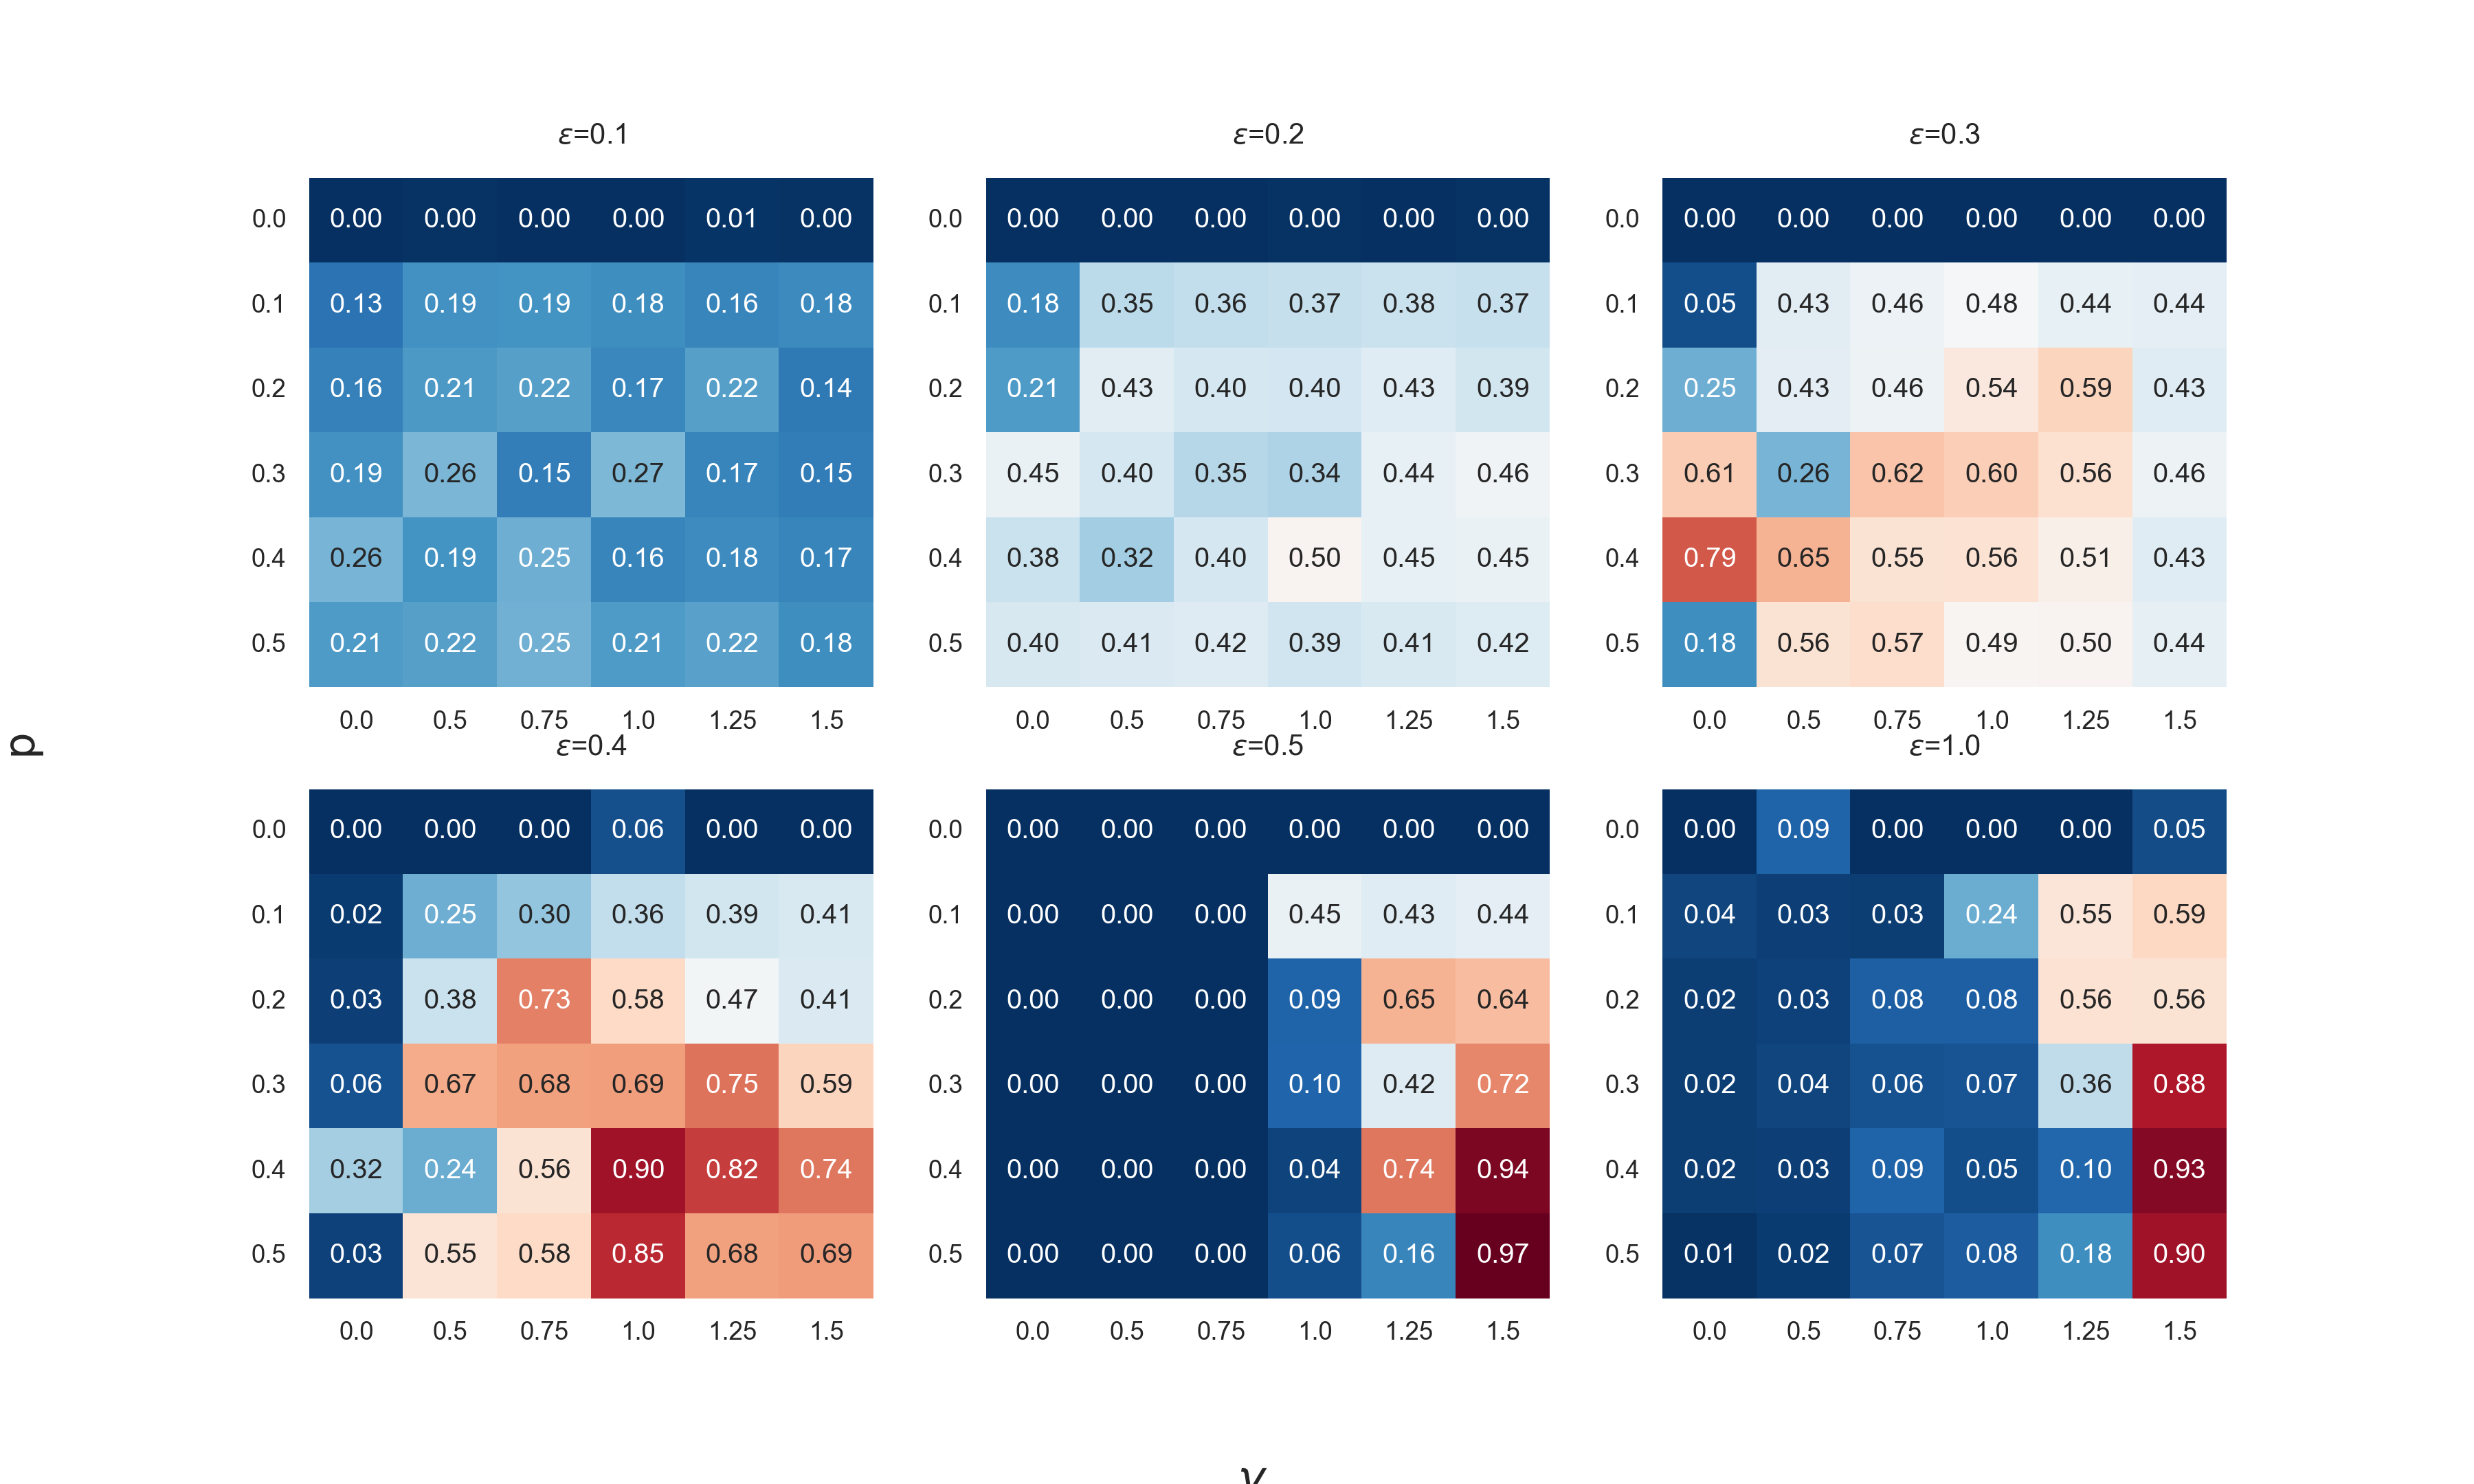
\includegraphics{figures/hm media mo0.05;0.5;0.95 perc_05 groupedby_eps.png}
    \caption{\textbf{Percentage of nodes around the middle media.}}
    \label{fig:3mediaperc05byeps}
\end{figure}

\begin{figure}
    \centering
    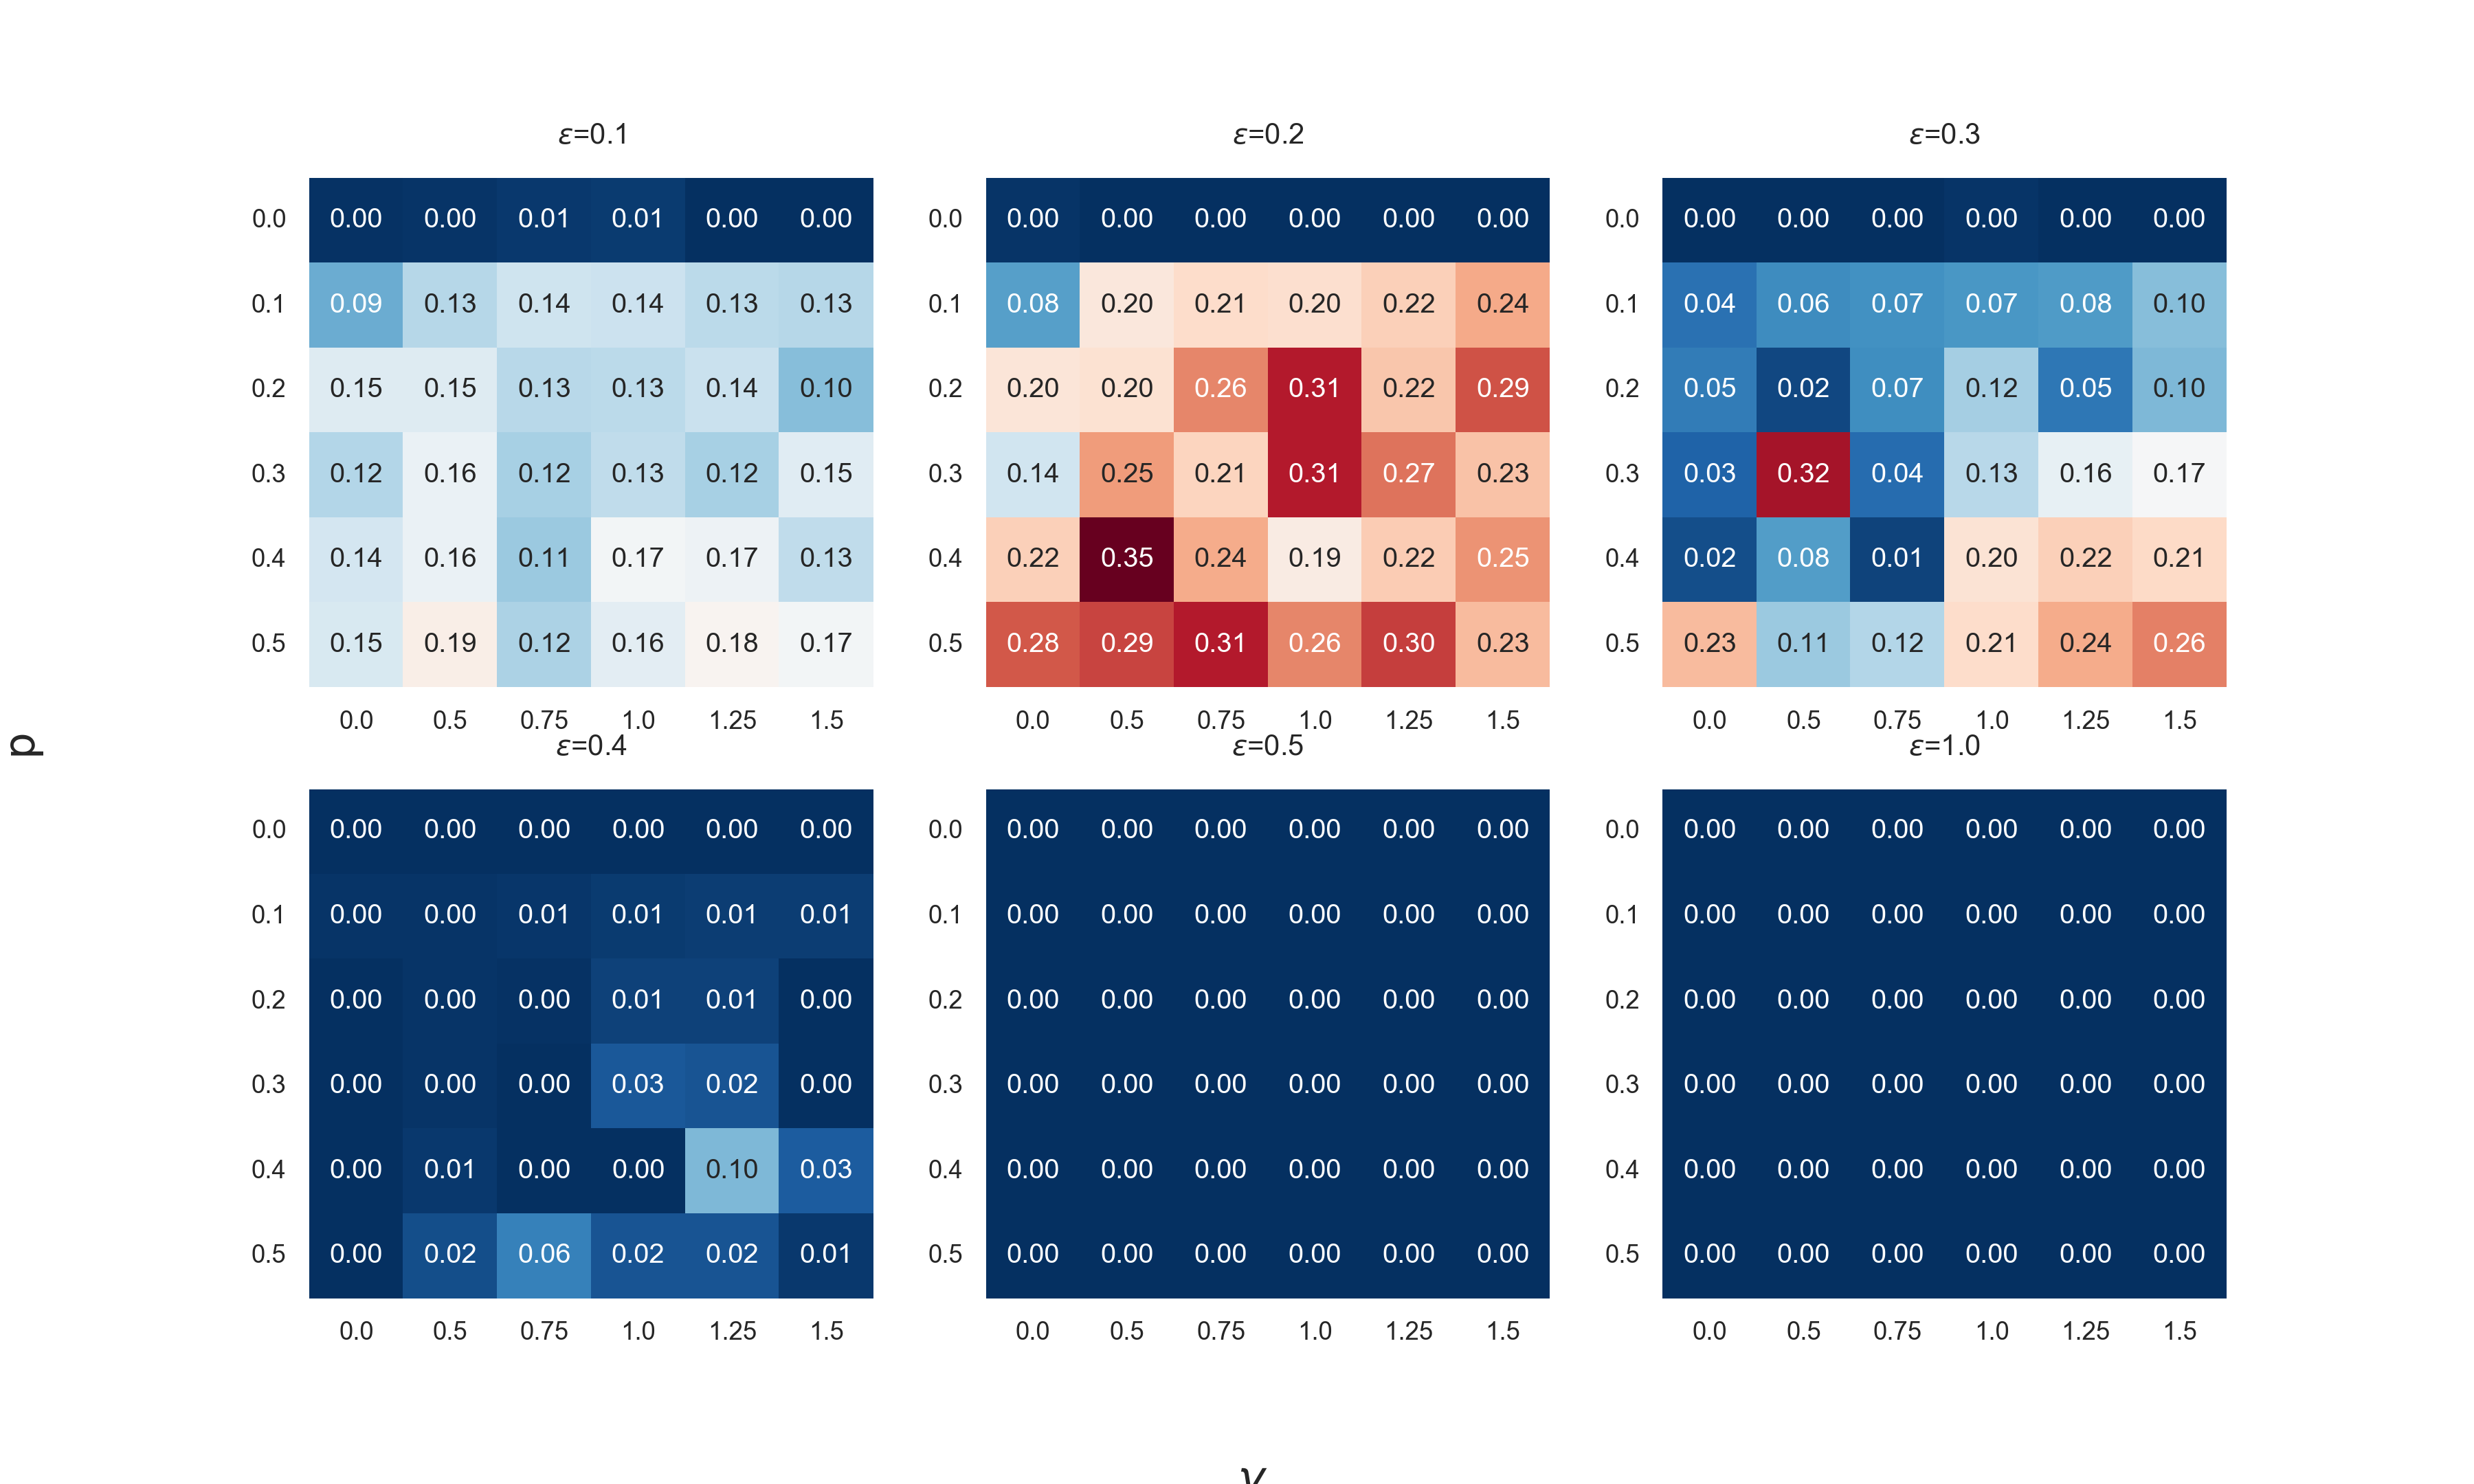
\includegraphics{figures/hm media mo0.05;0.5;0.95 perc_095 groupedby_eps.png}
    \caption{\textbf{Percentage of nodes around the higher extreme media.}}
    \label{fig:3mediaperc095byeps}
\end{figure}

\begin{figure}
    \centering
    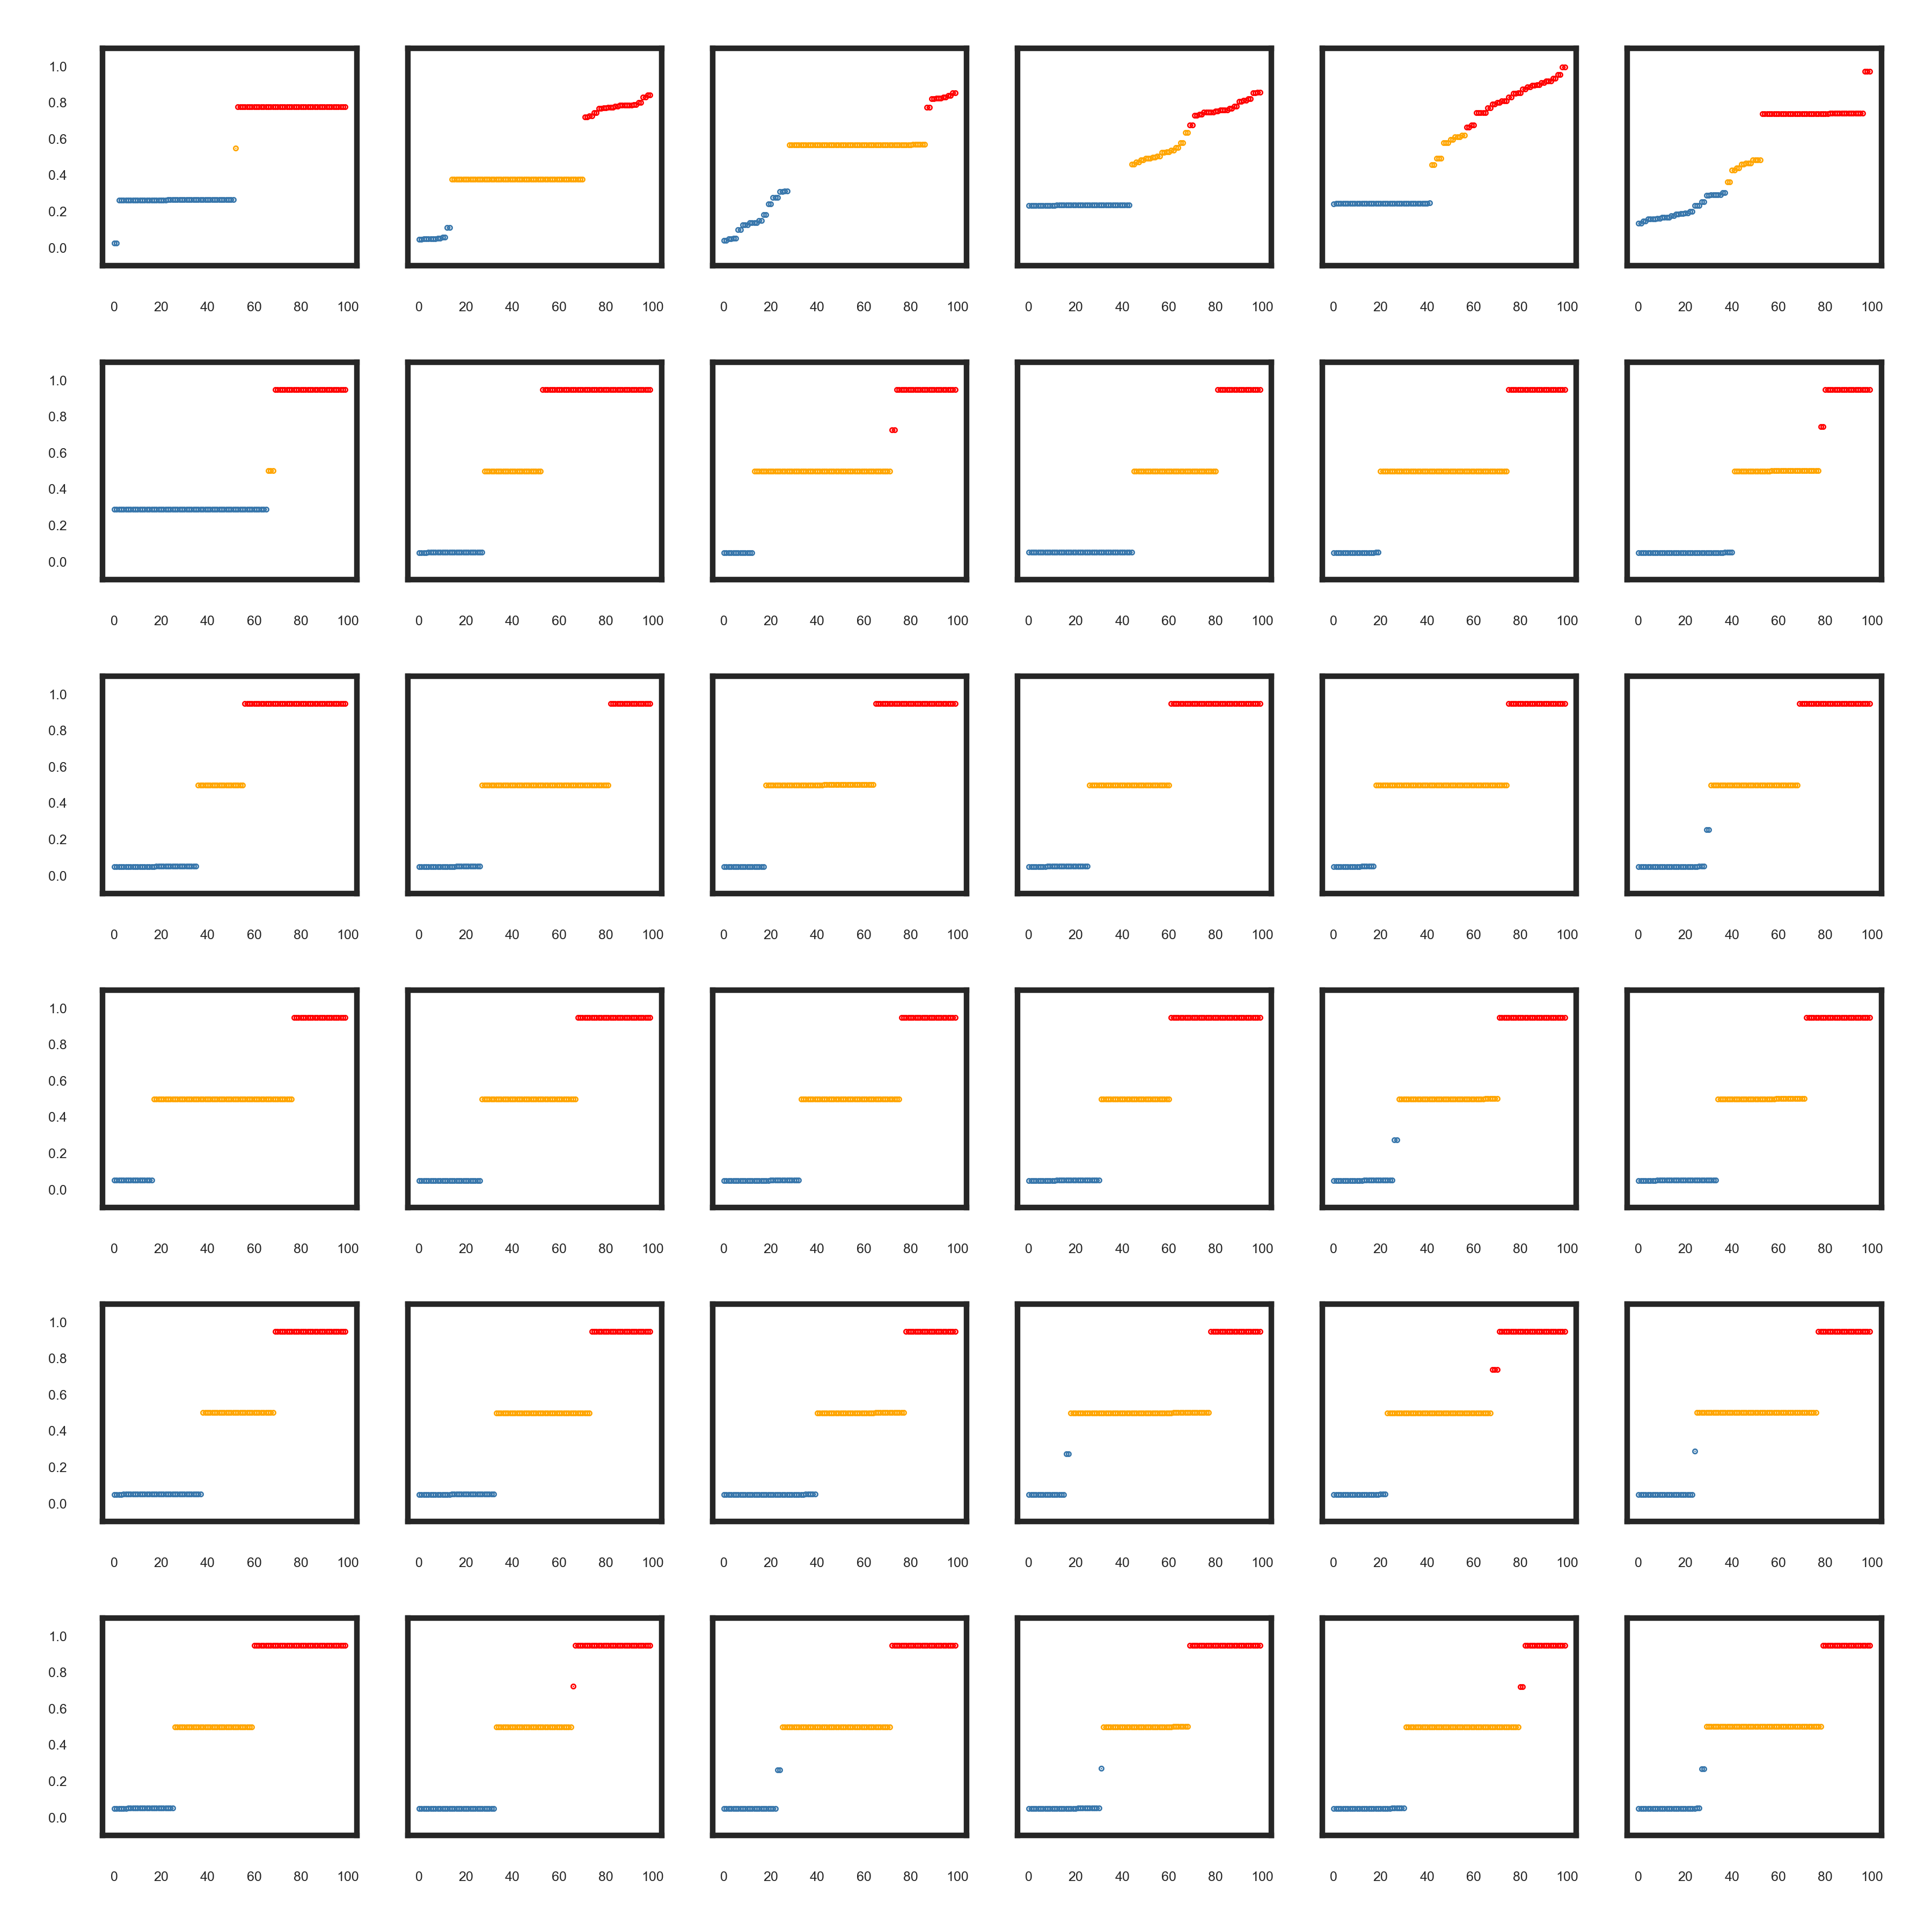
\includegraphics[width=0.8\textwidth]{figures/distributiongrid media mo[0.05, 0.5, 0.95] e0.2.png}
    \caption{\textbf{Examples of final opinion distributions in the case of three media for $\epsilon=0.2$ as a function of $\gamma$ and $p_m$.} In this case where $\epsilon=0.2$ we can see that without media the population that initially split in two clusters now normally presents one dense cluster while the other agents are distributed in a sparser fashion instead of forming another compact cluster (like in the case with no bias). As the probability to interact with the media grows, the clusters go from two to three and form around the media opinions.}
    \label{fig:3mediafinaldisteps02}
\end{figure}

\begin{figure}
    \centering
    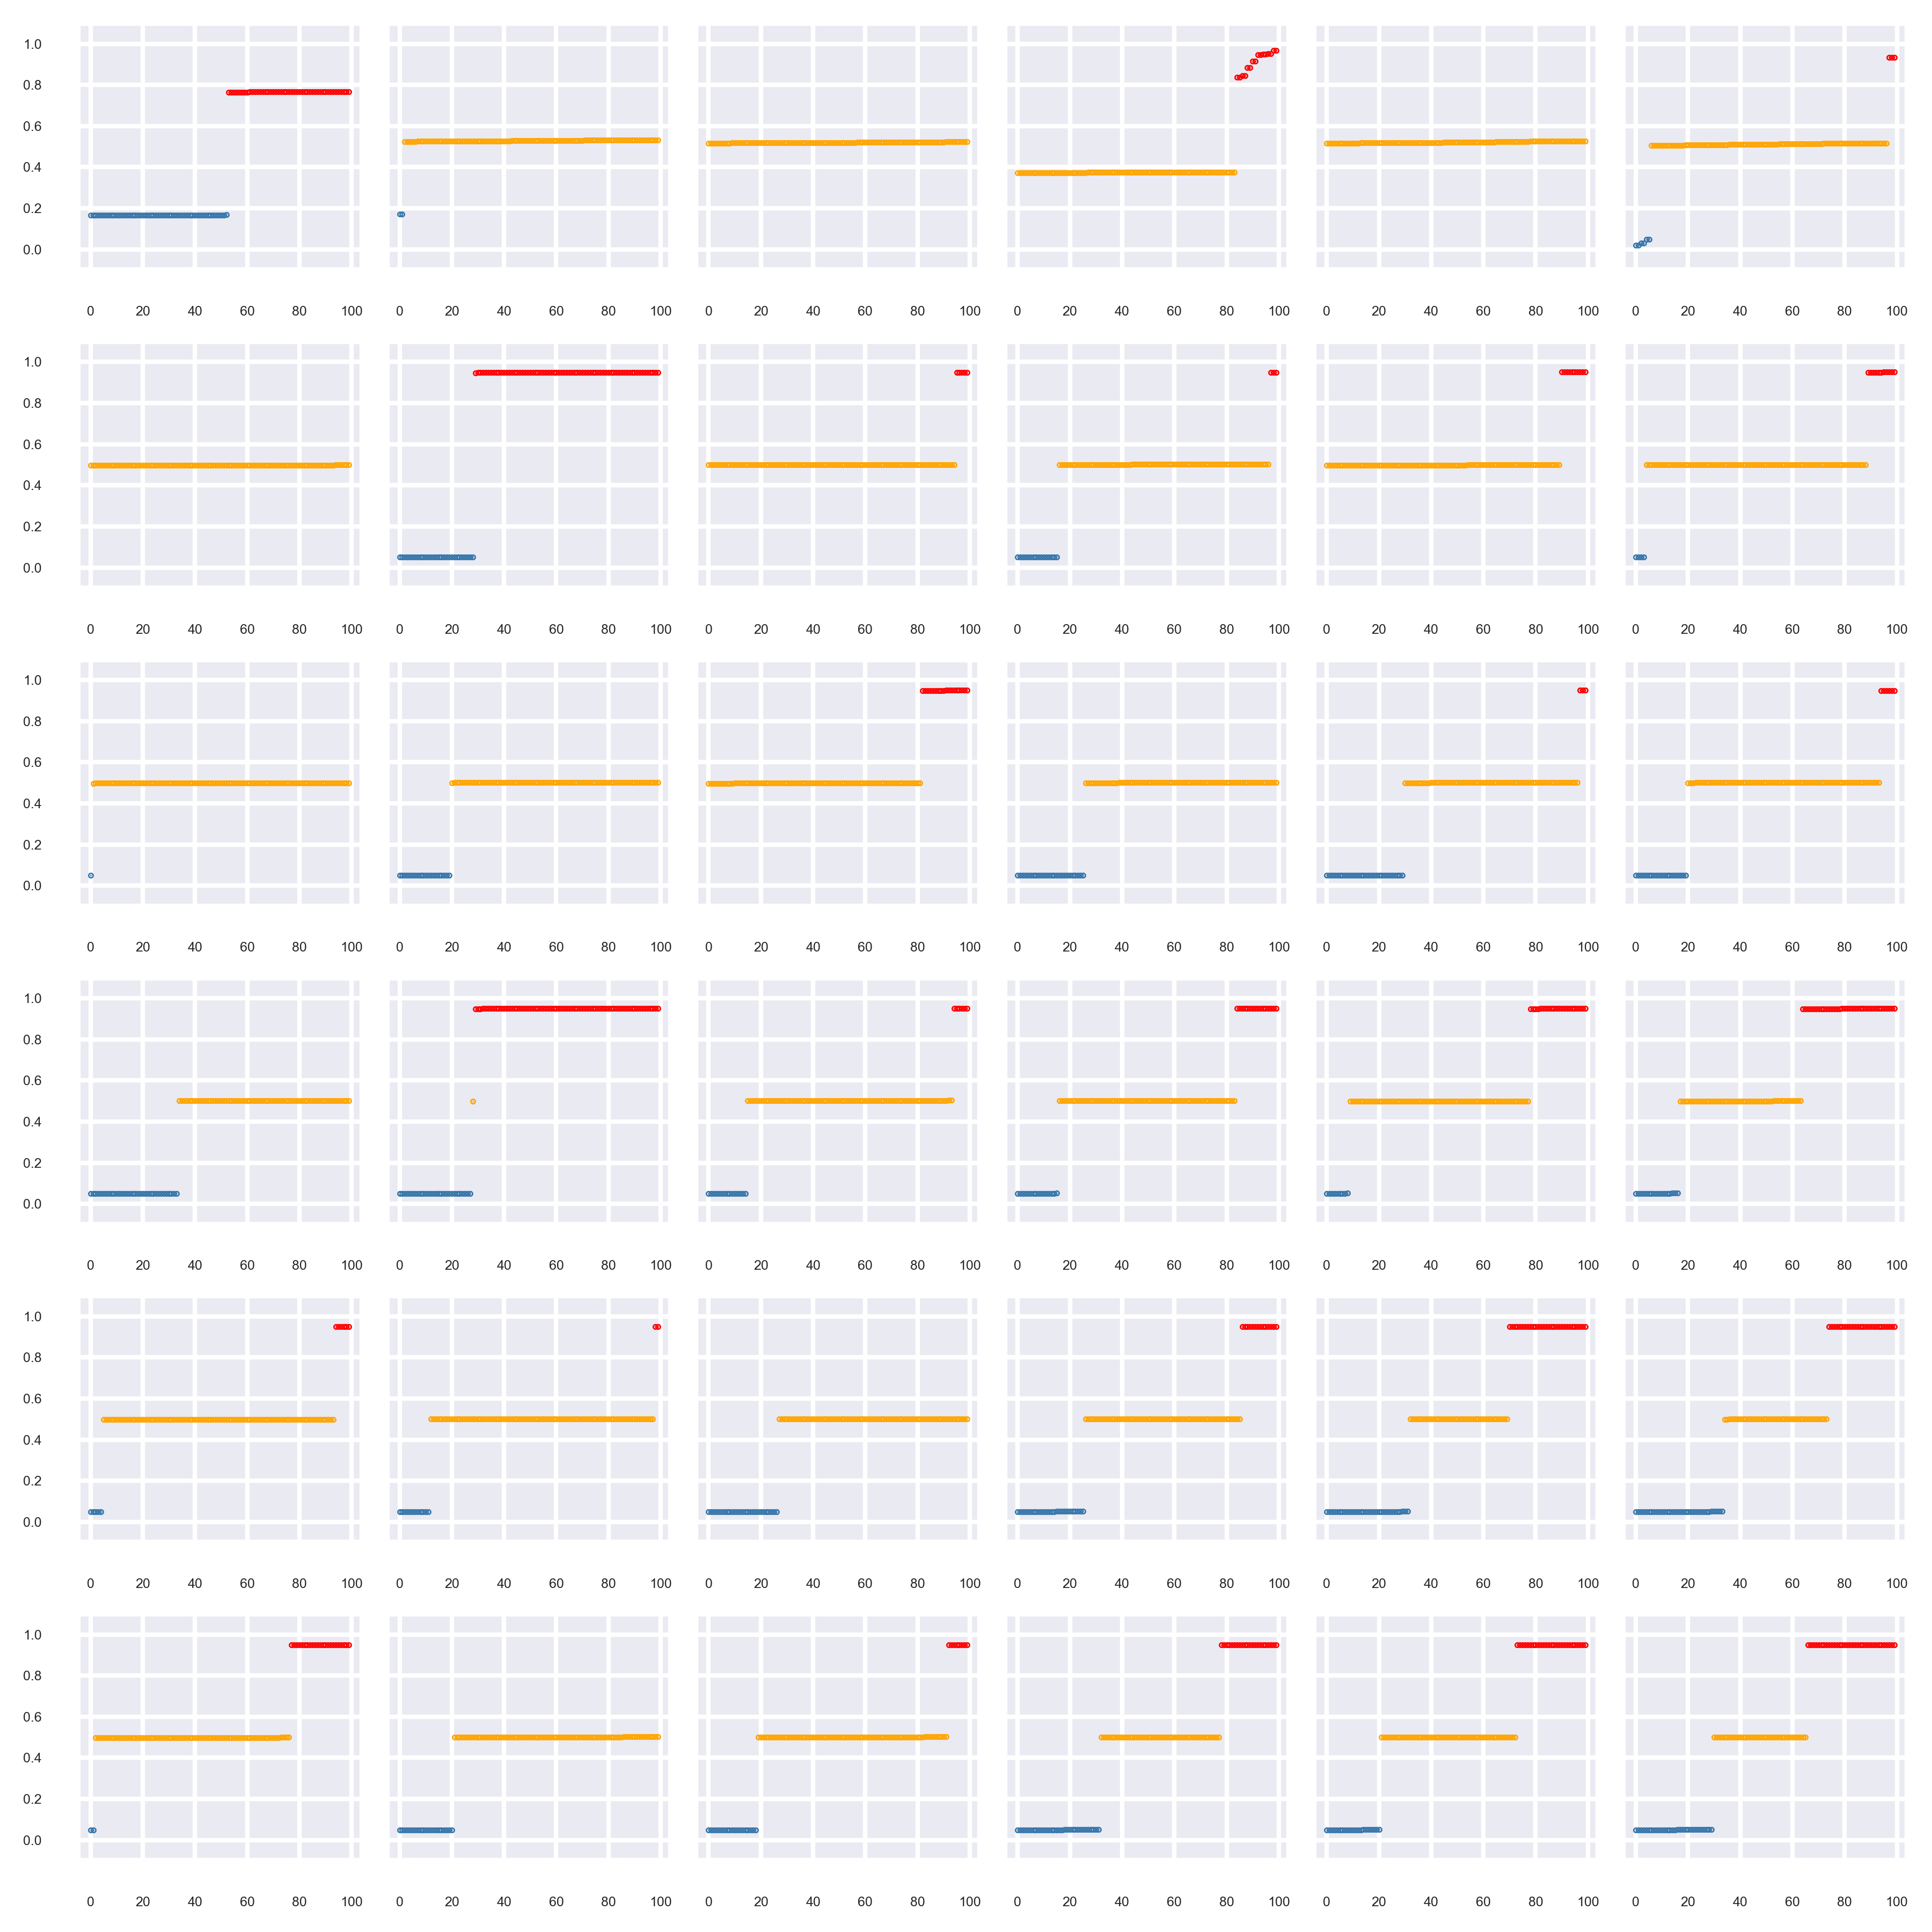
\includegraphics[width=0.8\textwidth]{figures/distributiongrid media mo[0.05, 0.5, 0.95] e0.3.png}
    \caption{\textbf{Examples of final opinion distributions in the case of three media for $\epsilon=0.3$ as a function of $\gamma$ and $p_m$.}}
    \label{fig:3mediafinaldisteps03}
\end{figure}

\begin{figure}
    \centering
    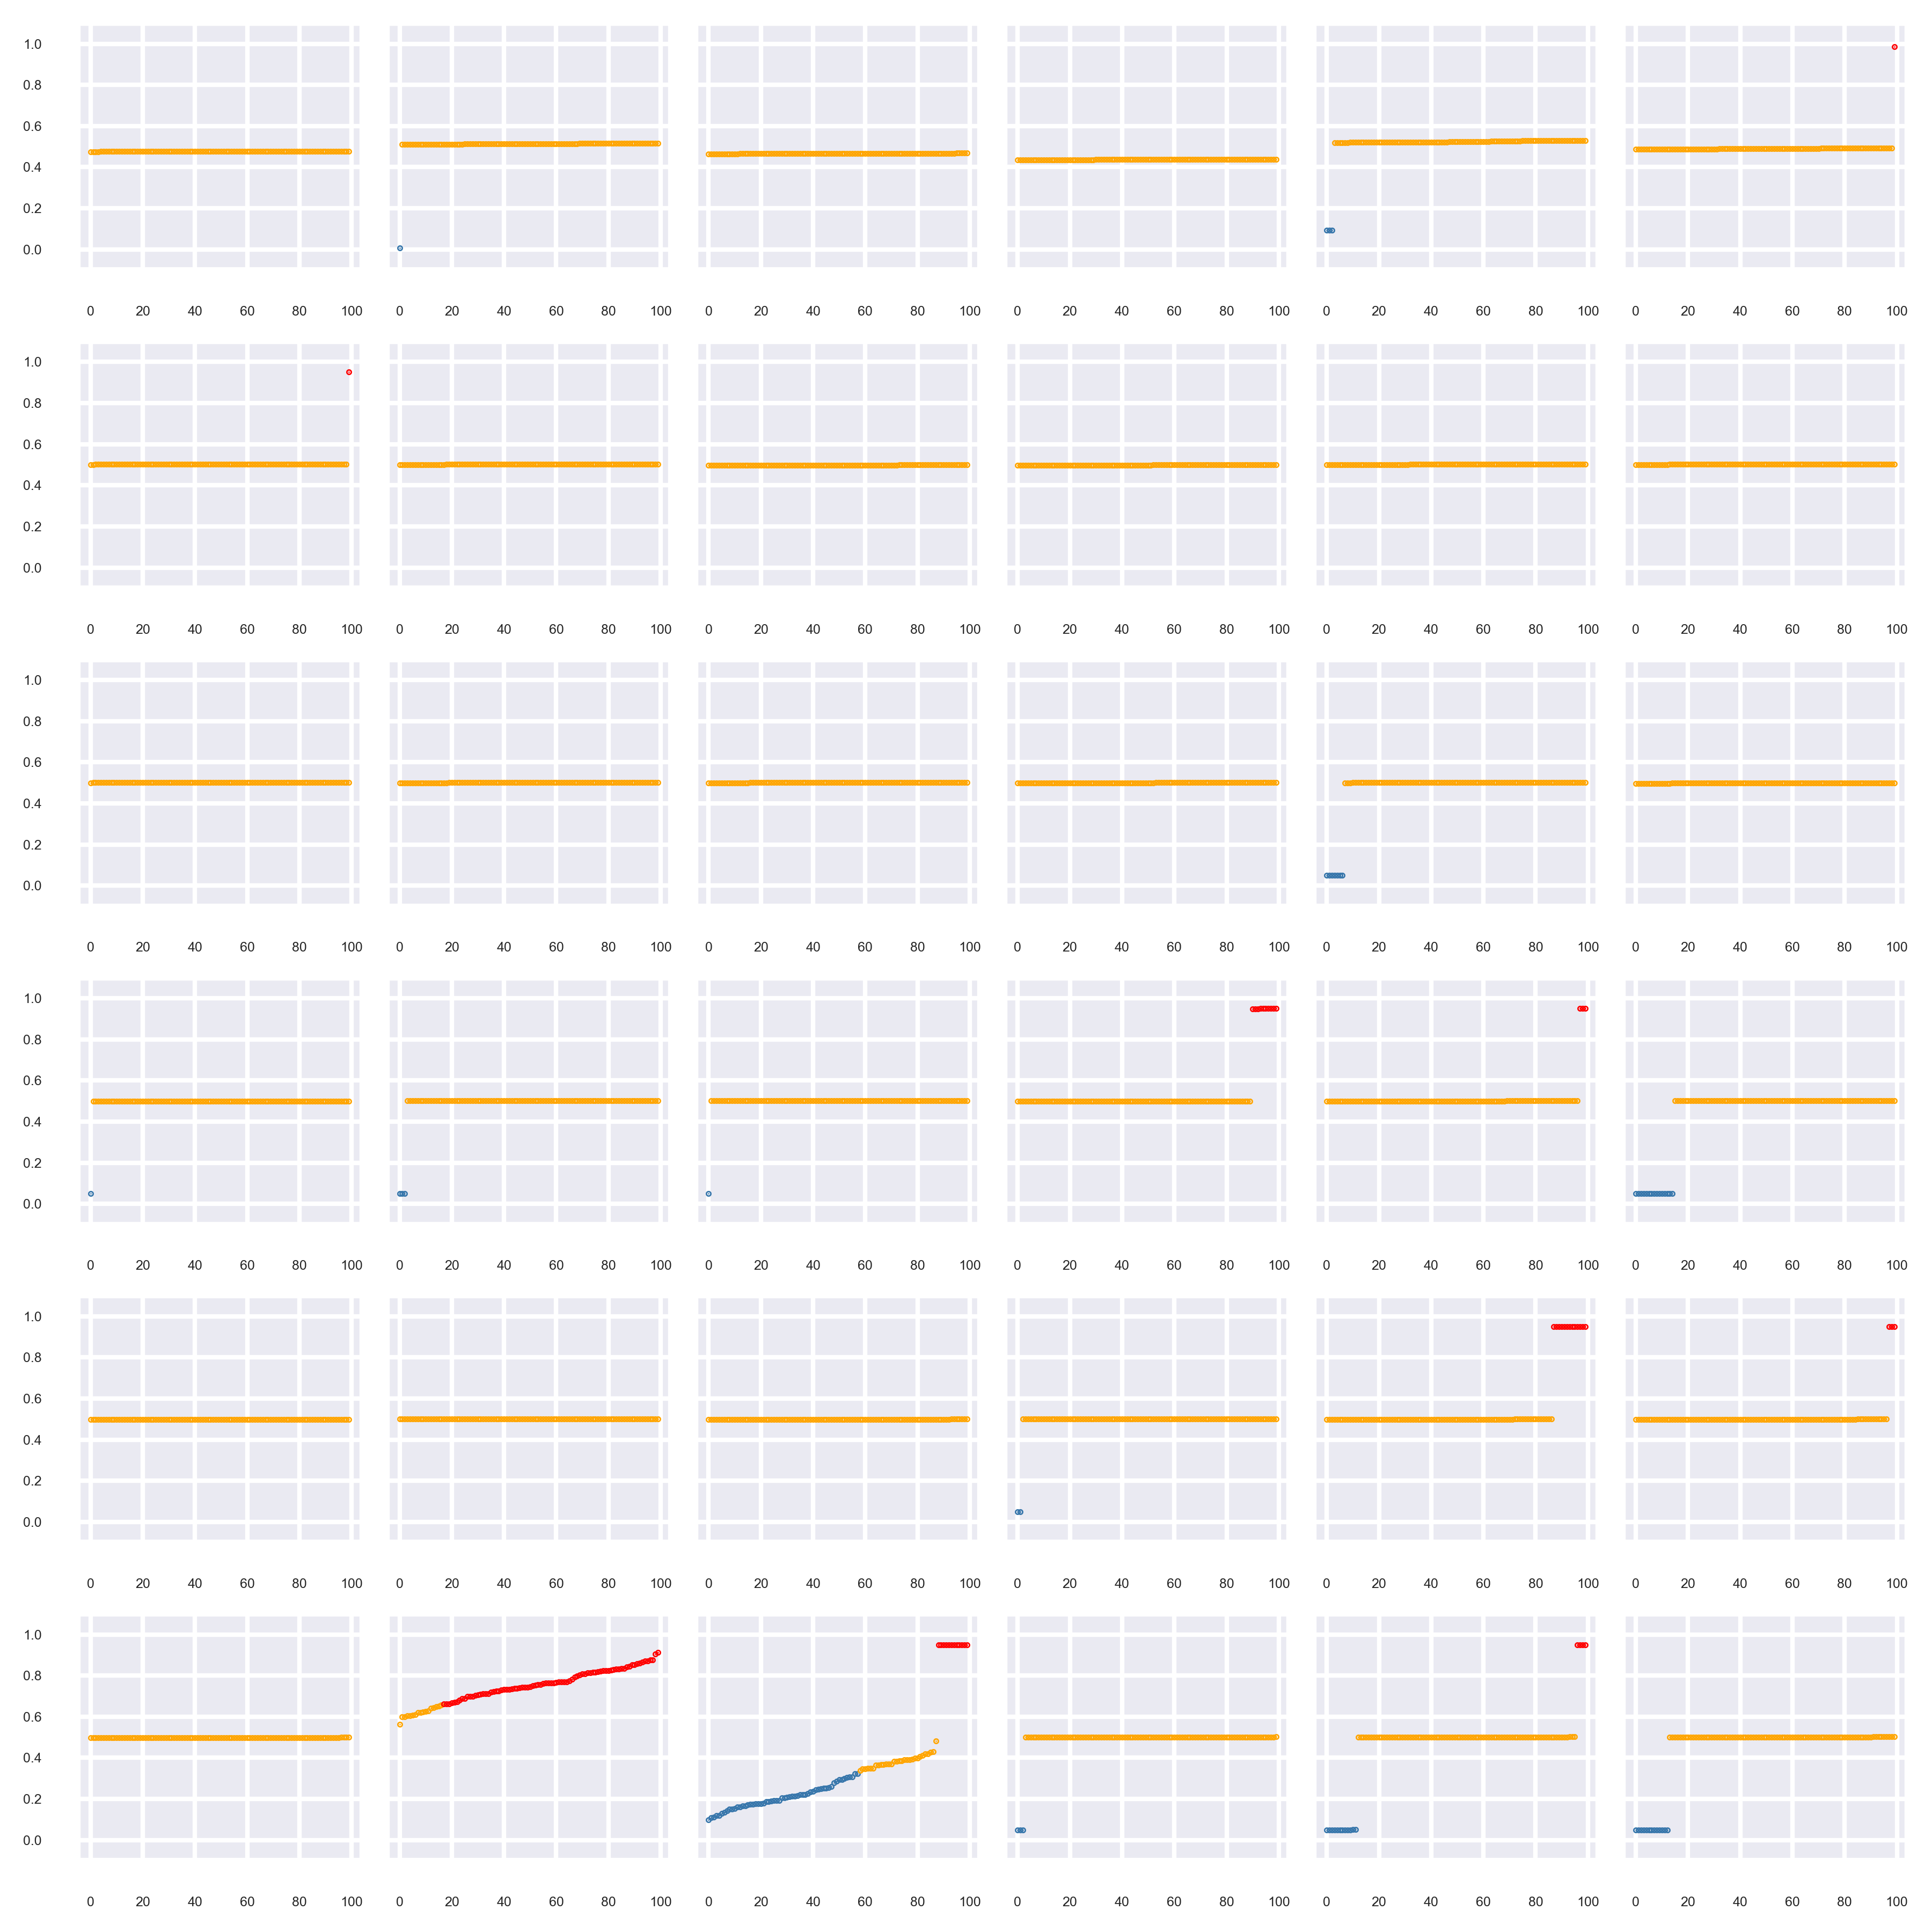
\includegraphics[width=0.8\textwidth]{figures/distributiongrid media mo[0.05, 0.5, 0.95] e0.4.png}
    \caption{\textbf{Examples of final opinion distributions in the case of three media for $\epsilon=0.4$ as a function of $\gamma$ and $p_m$.}}
    \label{fig:3mediafinaldisteps04}
\end{figure}

\begin{figure}
    \centering
    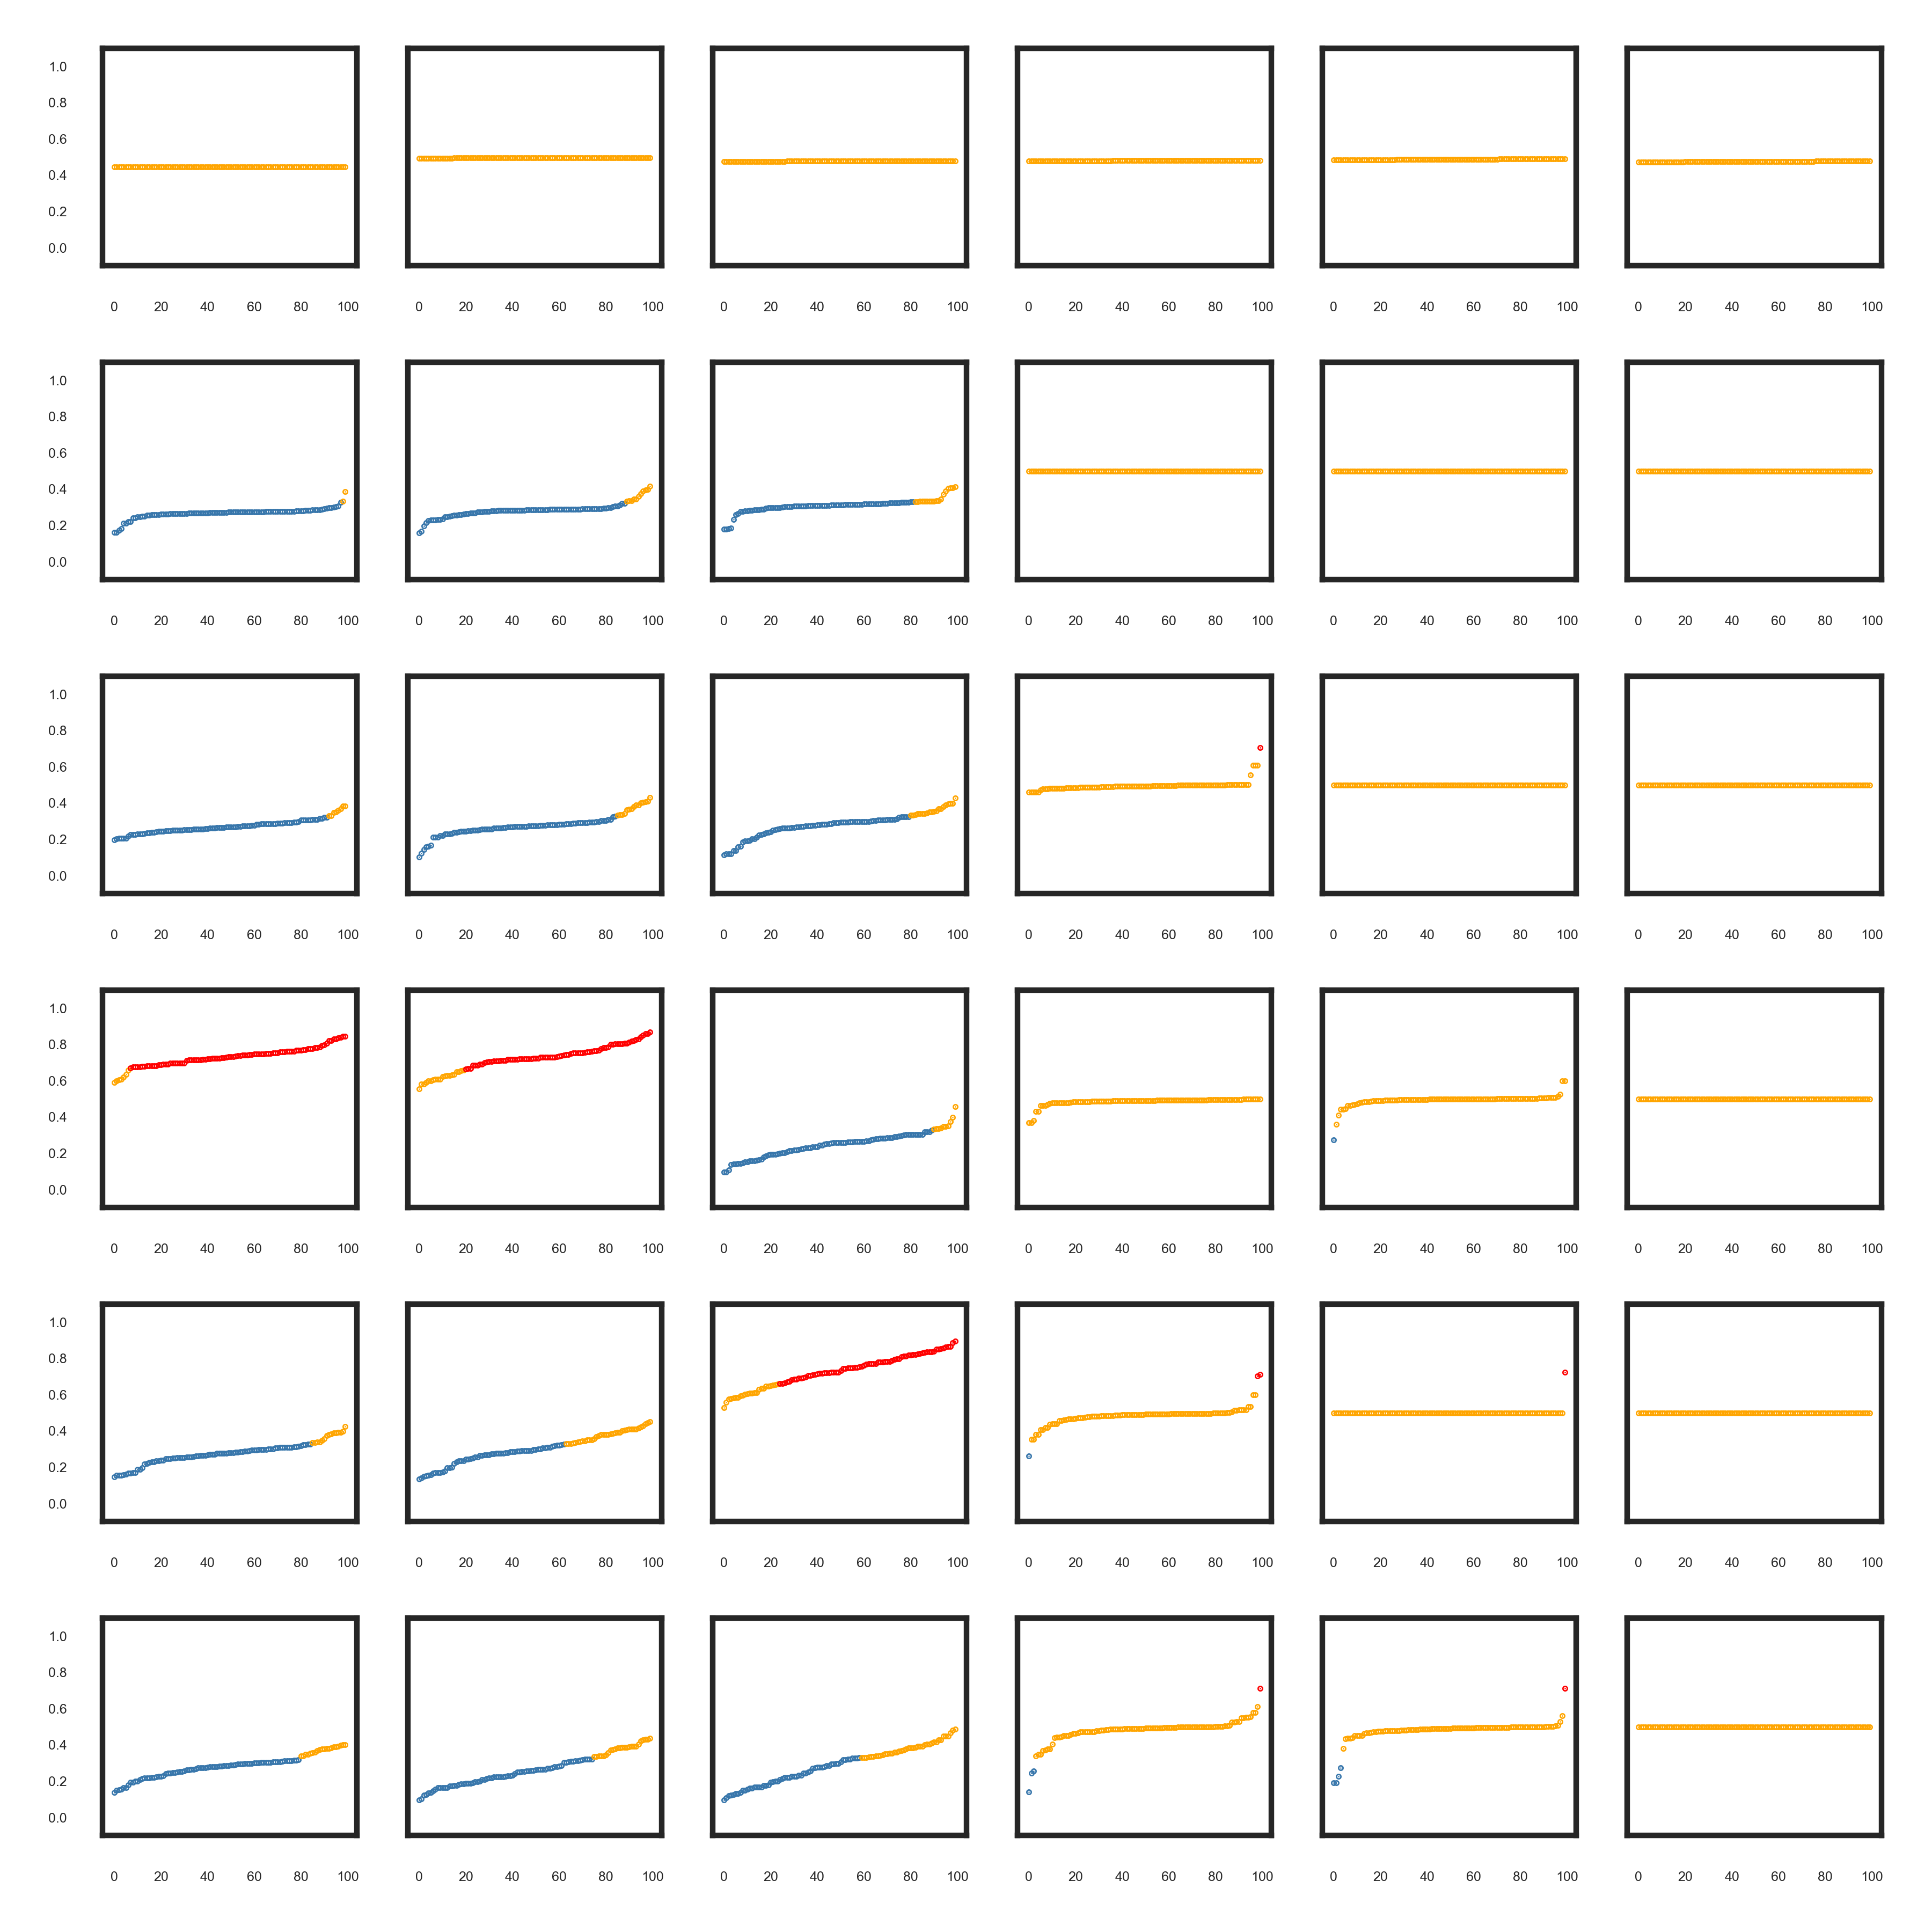
\includegraphics[width=0.8\textwidth]{figures/distributiongrid media mo[0.05, 0.5, 0.95] e0.5.png}
    \caption{\textbf{Examples of final opinion distributions in the case of three media for $\epsilon=0.5$ as a function of $\gamma$ and $p_m$.}}
    \label{fig:3mediafinaldisteps05}
\end{figure}

\begin{figure}
    \centering
    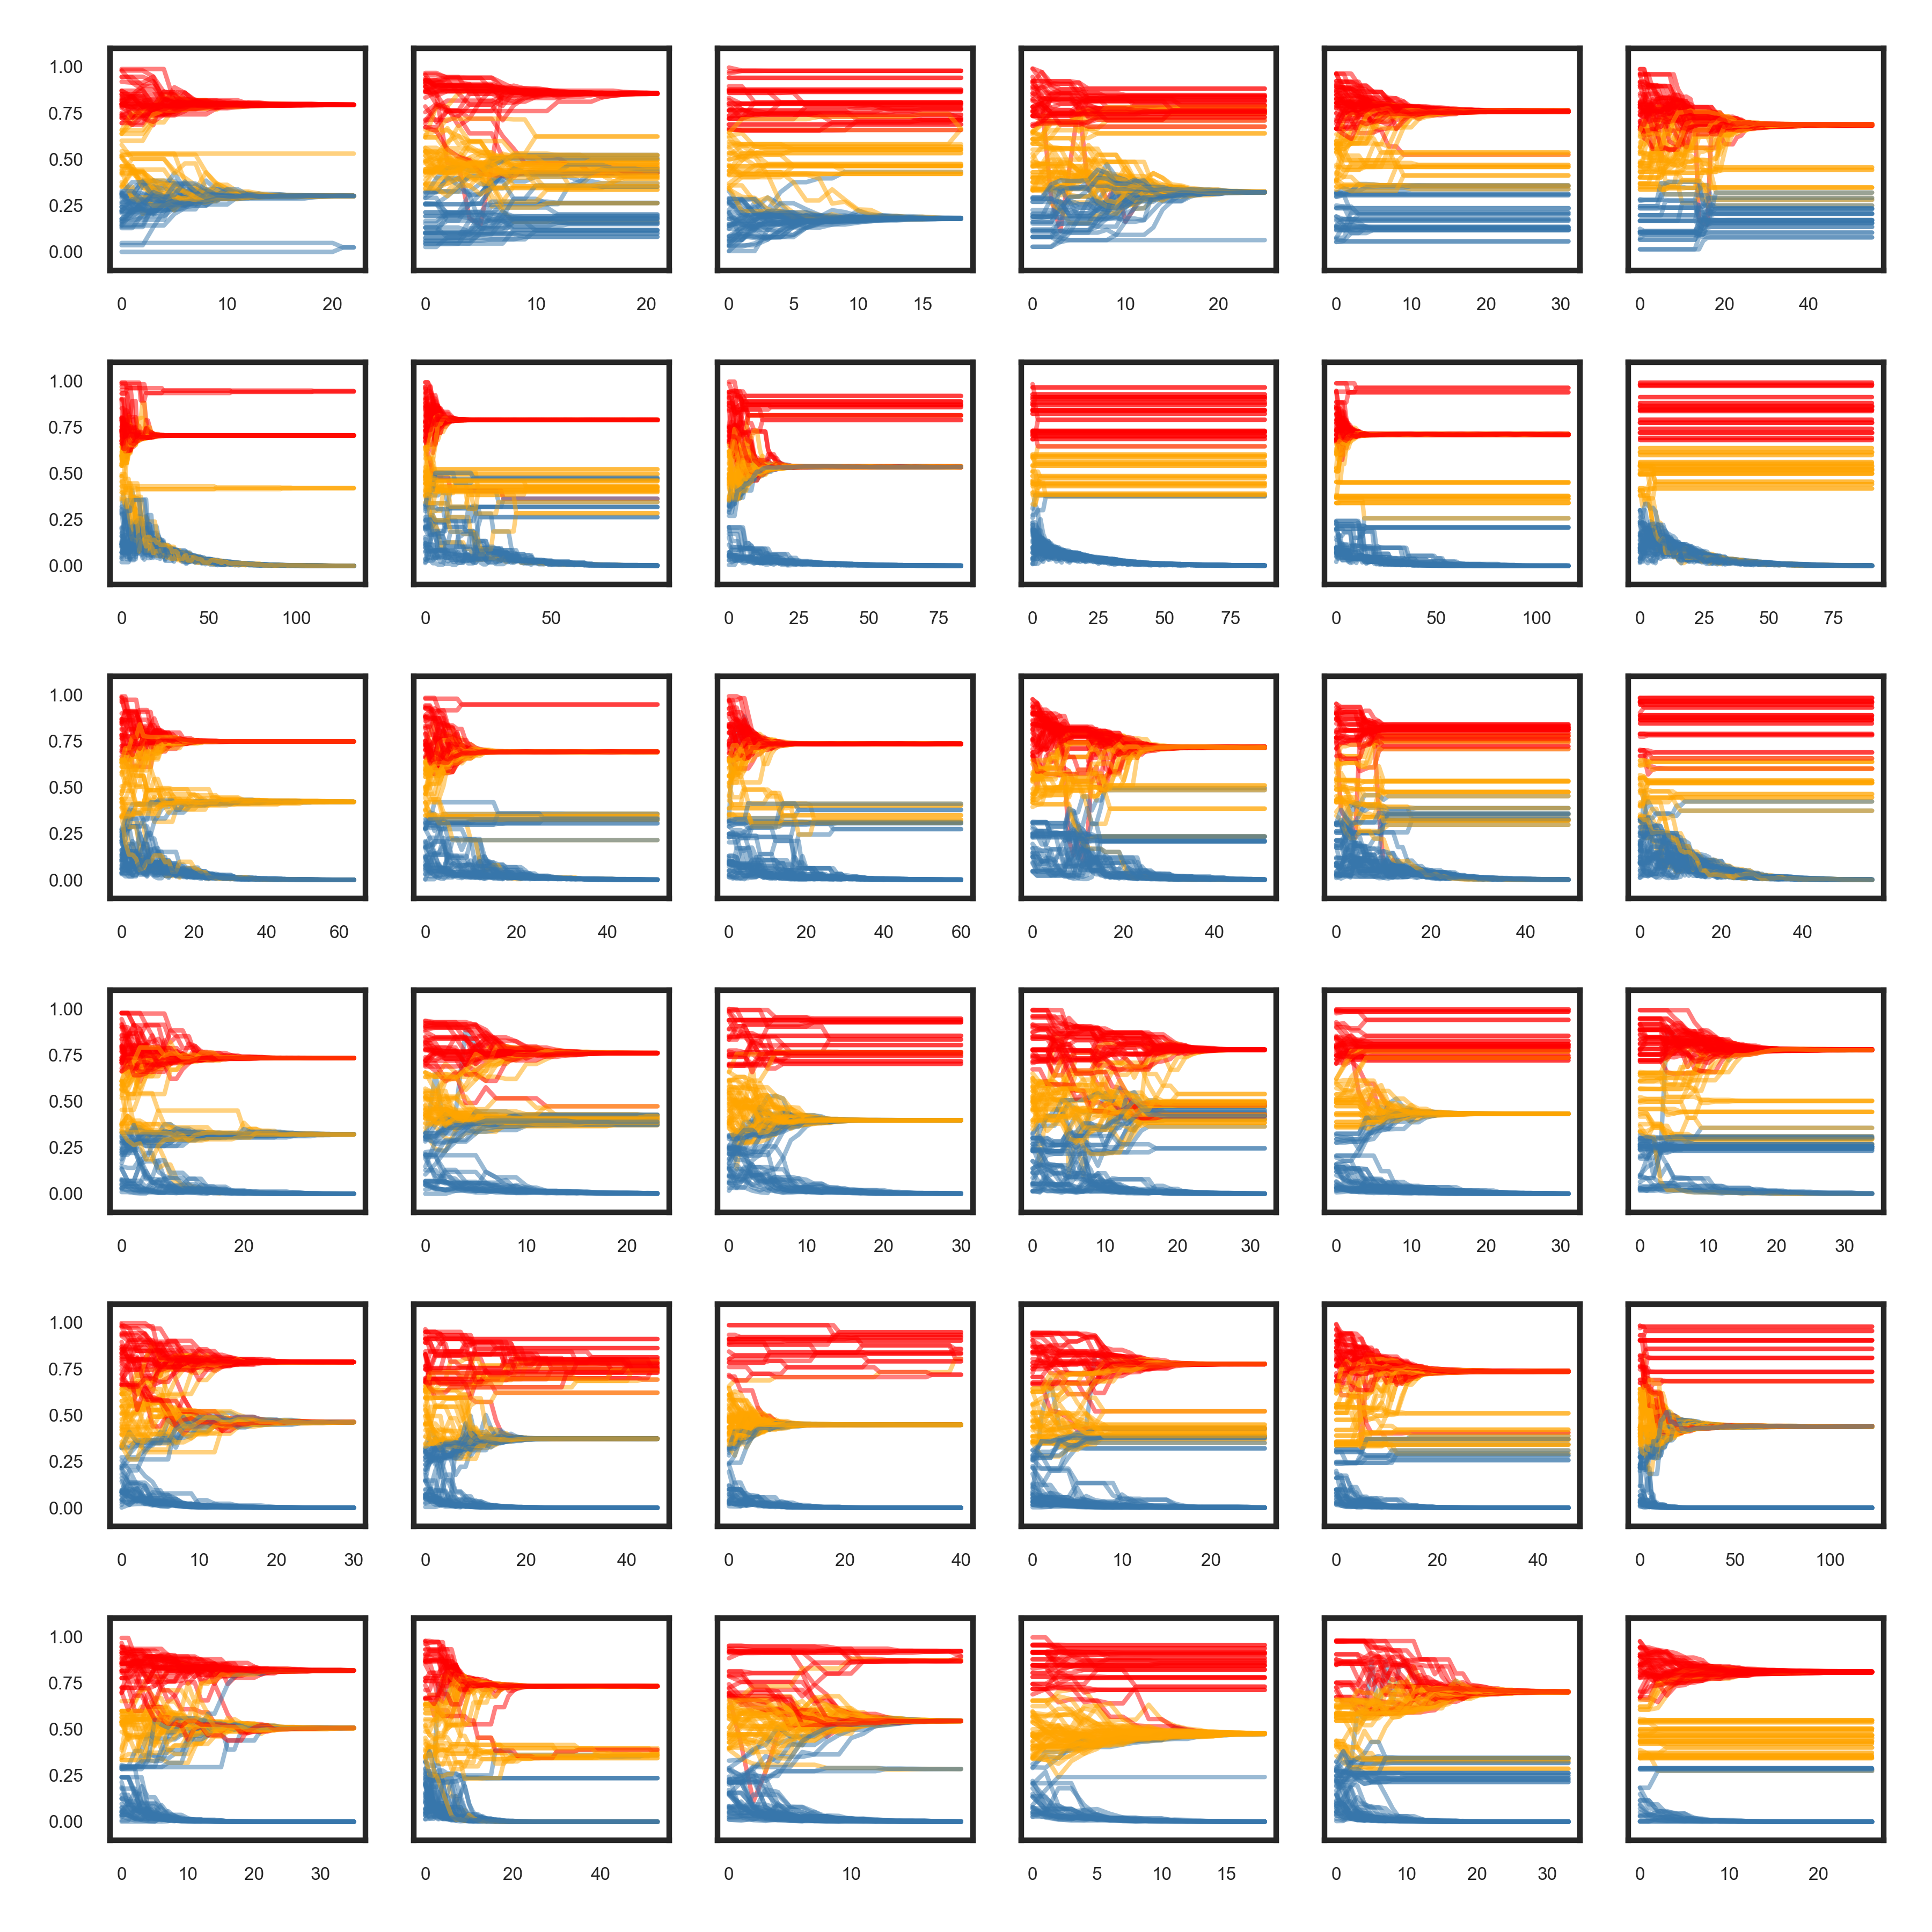
\includegraphics[width=\textwidth]{figures/evolutiongrid media mo[0.0] e0.2.png}
    \caption{\textbf{Examples of opinion evolution in the case of one extreme media for $\epsilon=0.2$ as a function of $\gamma$ and $p_m$}}
    \label{fig:00evolutioneps02}
\end{figure}

\begin{figure}
    \centering
    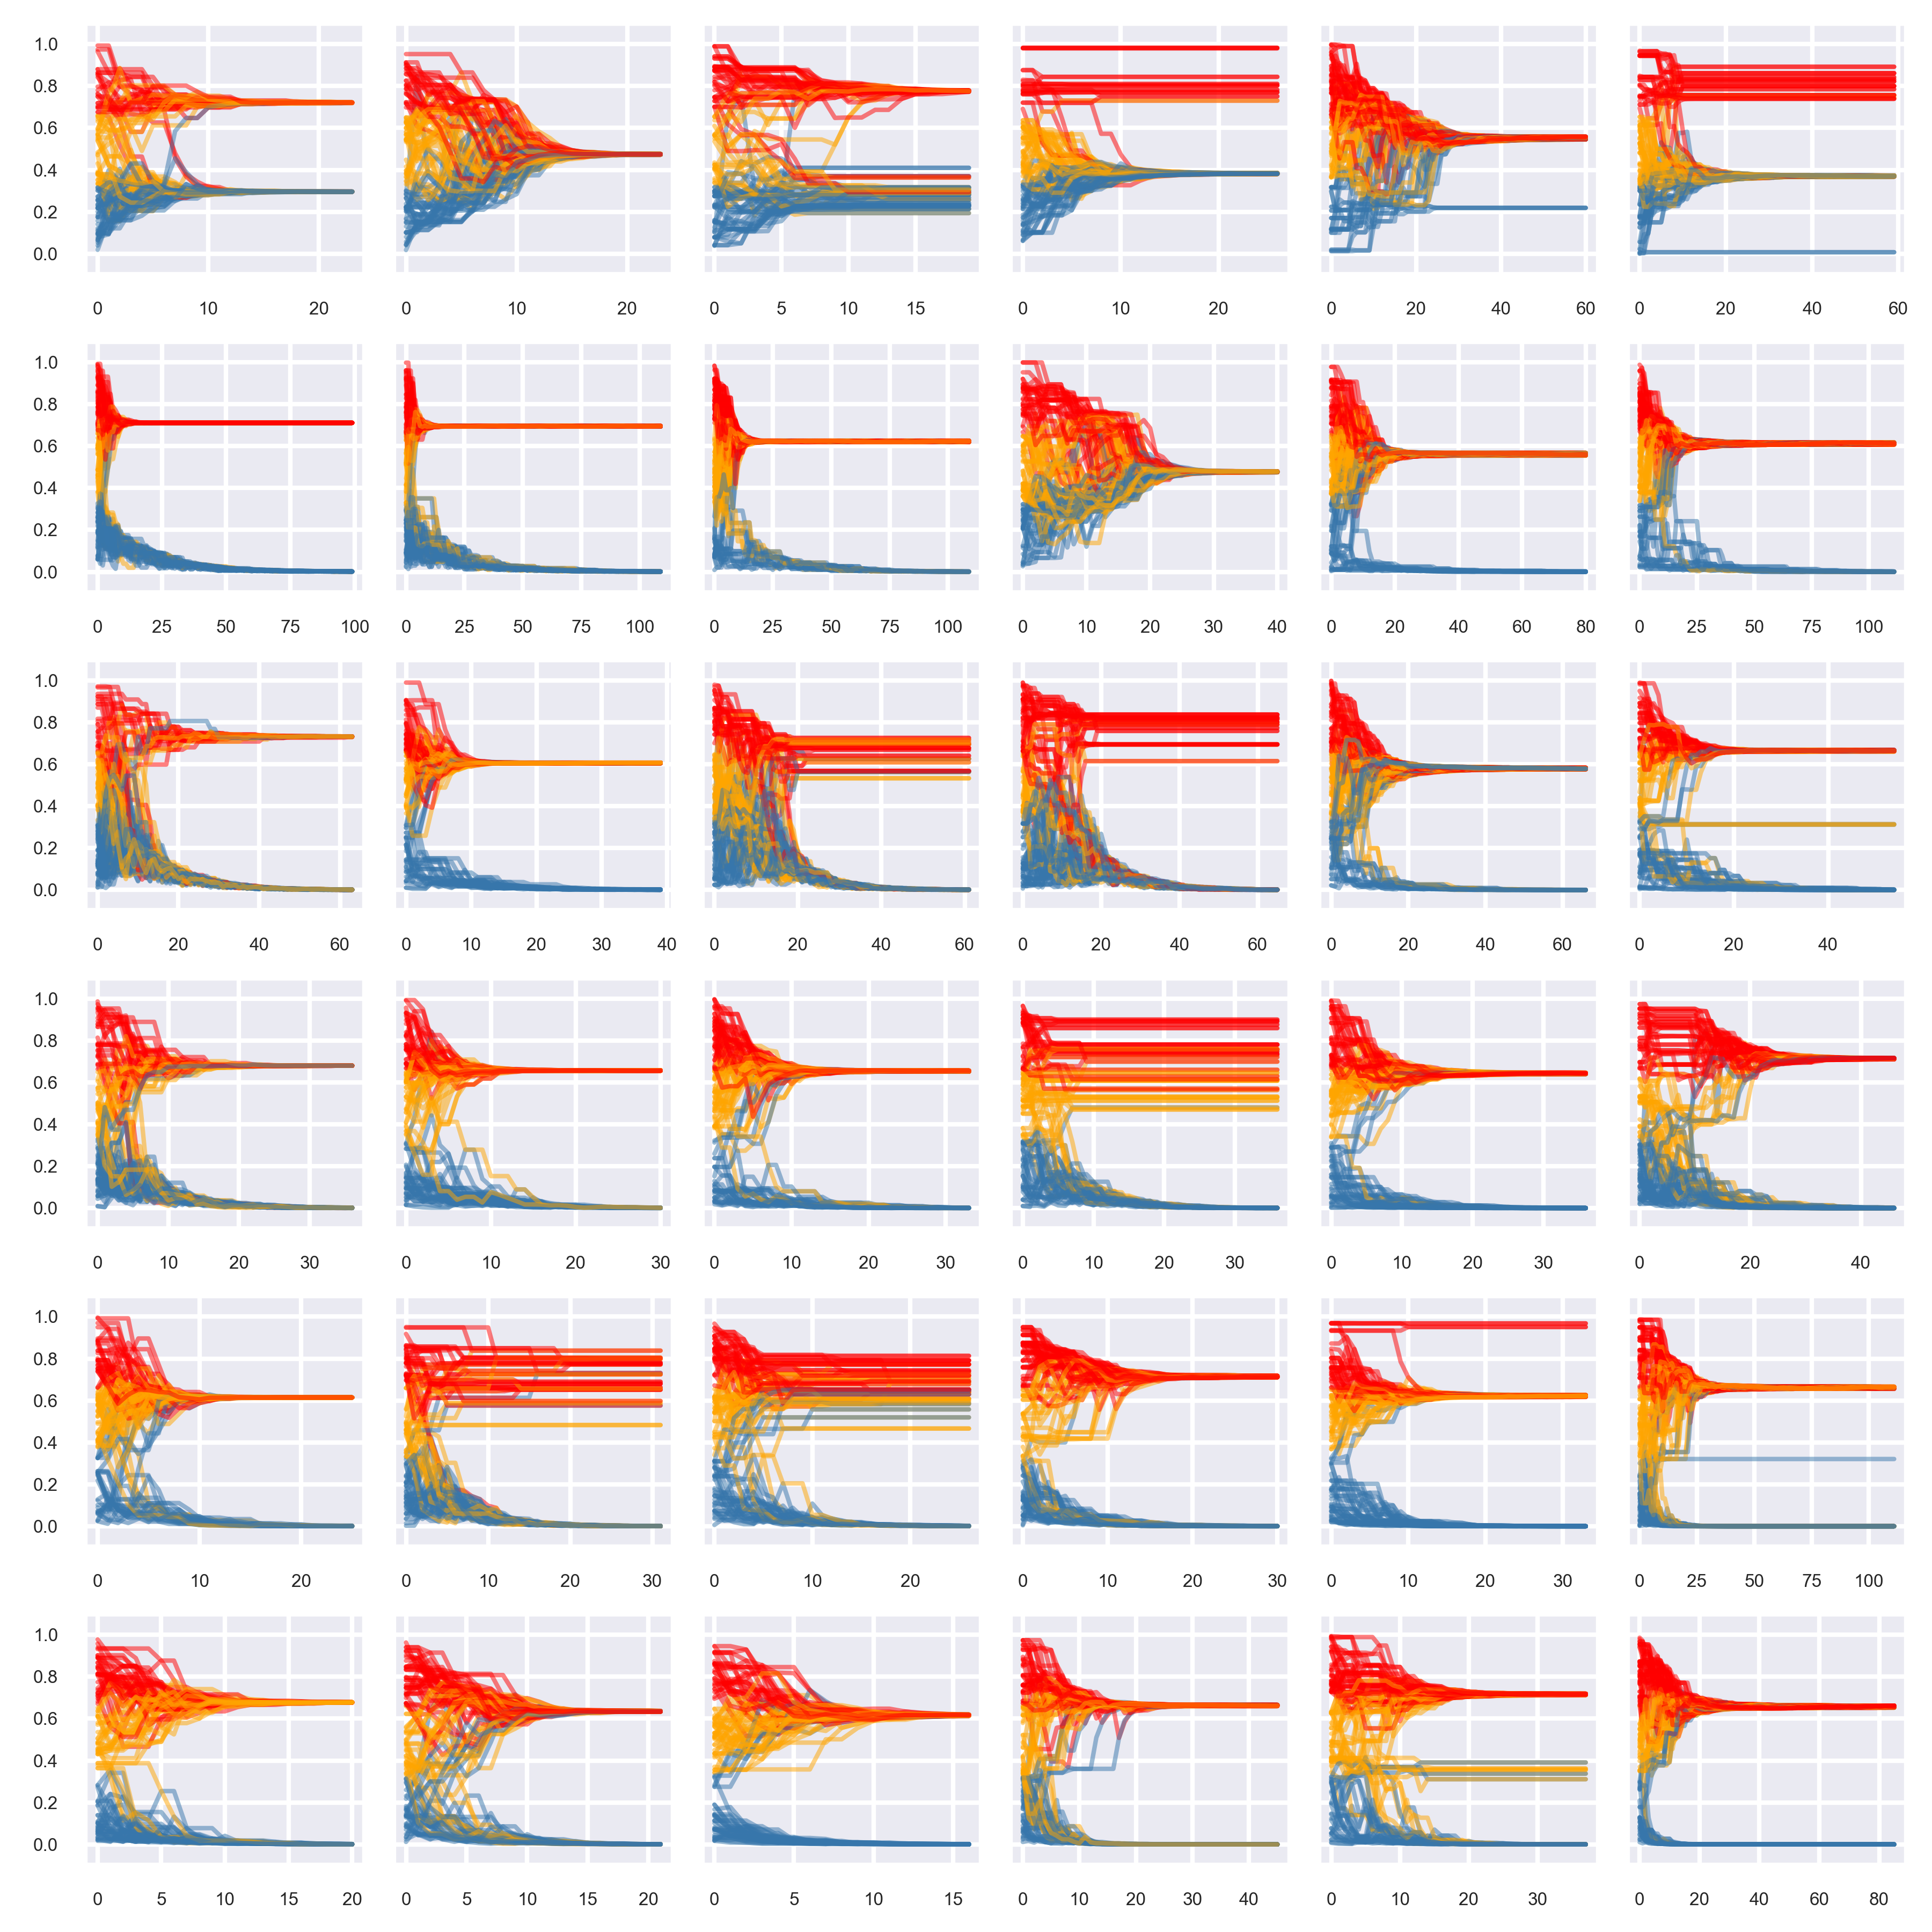
\includegraphics[width=\textwidth]{figures/evolutiongrid media mo[0.0] e0.3.png}
    \caption{\textbf{Examples of opinion evolution in the case of one extreme media for $\epsilon=0.3$ as a function of $\gamma$ and $p_m$}}
    \label{fig:00evolutioneps03}
\end{figure}

\begin{figure}
    \centering
    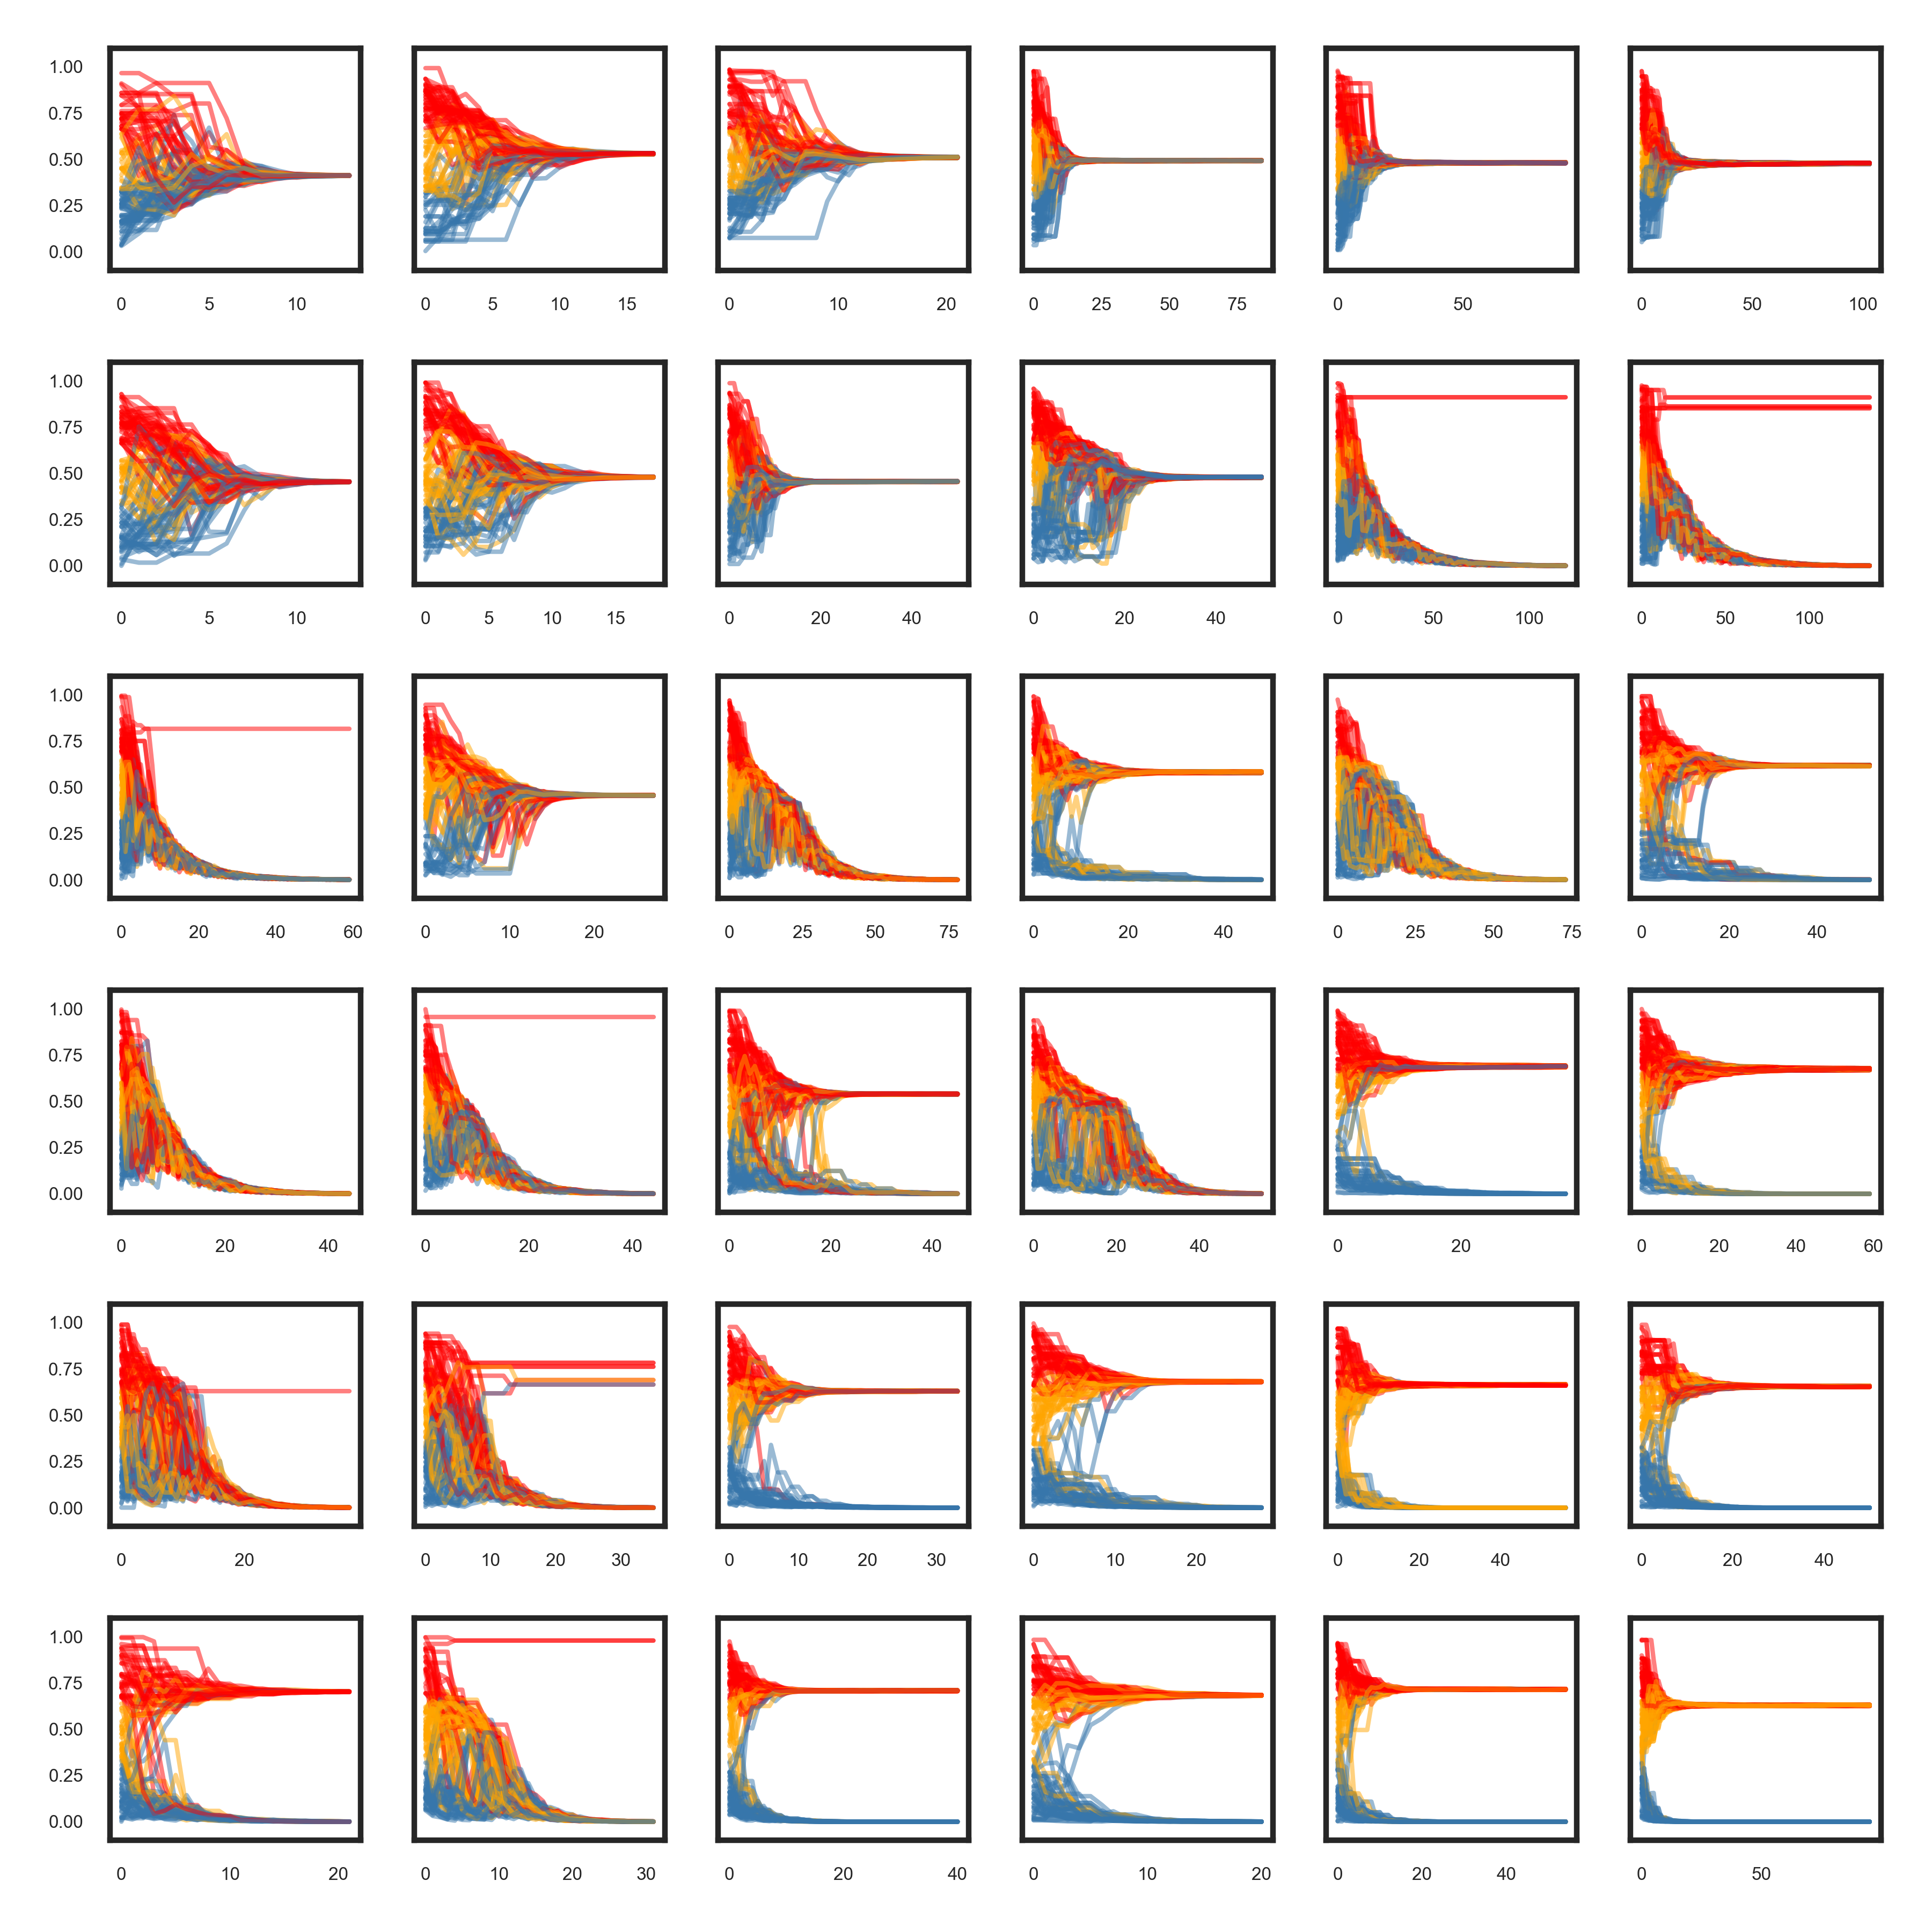
\includegraphics[width=\textwidth]{figures/evolutiongrid media mo[0.0] e0.4.png}
    \caption{\textbf{Examples of opinion evolution in the case of one extreme media for $\epsilon=0.4$ as a function of $\gamma$ and $p_m$}}
    \label{fig:00evolutioneps04}
\end{figure}

\begin{figure}
    \centering
    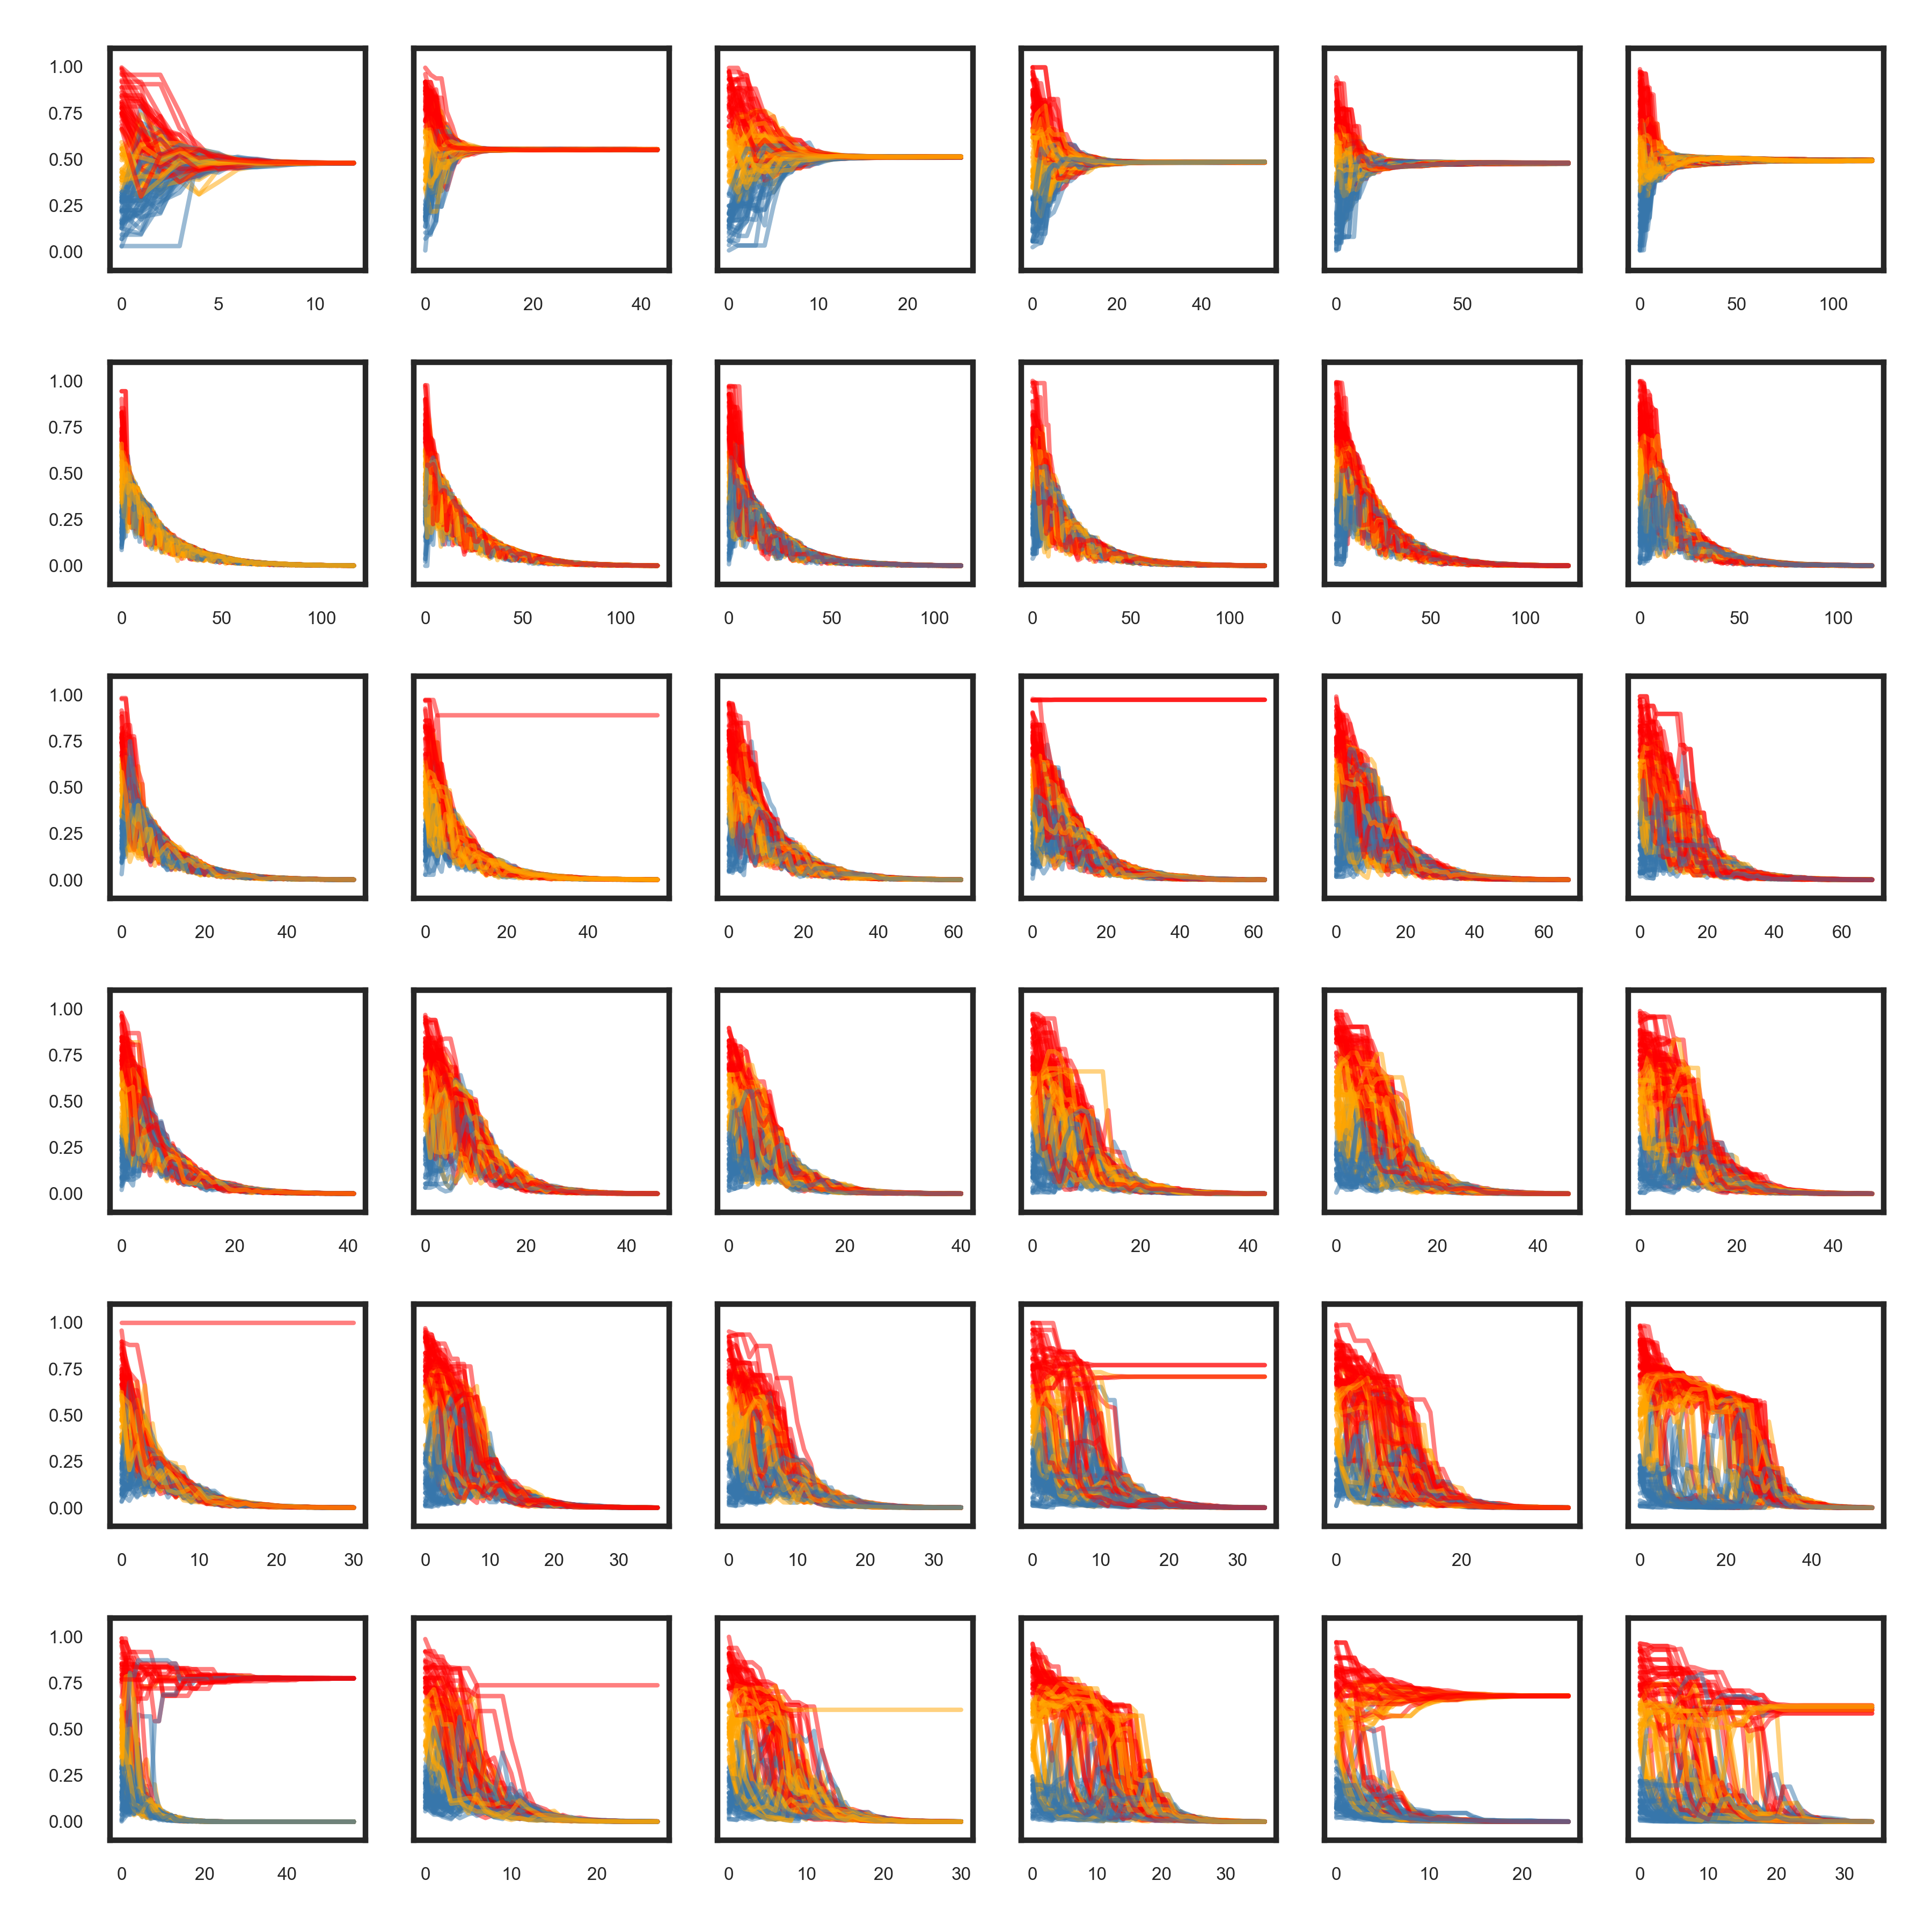
\includegraphics[width=\textwidth]{figures/evolutiongrid media mo[0.0] e0.5.png}
    \caption{\textbf{Examples of opinion evolution in the case of one extreme media for $\epsilon=0.5$ as a function of $\gamma$ and $p_m$}}
    \label{fig:00evolutioneps05}
\end{figure}

\end{document}

